
\chapter{Preliminary Study for Hyperparameters Tuning}
\label{chap:hyperparameters_tuning}

The application of the $A^*$ search algorithm to the training of neural networks introduces a unique set of challenges that distinguish it fundamentally from traditional gradient-based optimization. While Gradient Descent operates in a continuous landscape, $A^*$ explores a discretized state-space of weights and biases, where the efficiency of the search is governed by the logic of neighbor generation and the management of computational resources.

This chapter details an extensive experimental campaign—spanning across various network complexities and architectural strategies—aimed at identifying the optimal balance between convergence precision and computational feasibility. Given the exponential growth of the search tree, a "vanilla" implementation of $A^*$ is insufficient for deep architectures. Consequently, this study evaluates several advanced techniques designed to mitigate the "curse of dimensionality" and prevent hardware exhaustion.

The tuning process is structured into four primary investigative areas:
\begin{enumerate}
    \item \textbf{Structural Adaptation:} Testing dynamic versus static kernel reshaping to simplify the architectural search space.
    \item \textbf{Search Resolution:} Analyzing adaptive quantization factors to allow the algorithm to refine its search as it approaches local minima.
    \item \textbf{Stochastic Exploration:} A grid search on random sampling parameters to evaluate the effectiveness of non-deterministic neighbor generation.
    \item \textbf{Resource Optimization:} The integration of Beam Search to transition from an exhaustive memory-heavy search to a resource-constrained optimization process.
\end{enumerate}

By evaluating these components across three distinct network scales, this study establishes a robust hyperparameter baseline that ensures the $A^*$ algorithm can effectively train neural networks within realistic hardware constraints.

\section{Experimental Setup}
\label{sec:experimental_setup}

To ensure that the results obtained across the various test phases are consistent and comparable, a standardized experimental environment was established. This setup focuses on isolating the effects of hyperparameter changes while keeping the dataset and evaluation metrics constant.

\subsection{Benchmark Dataset and Network Architectures}
The \textbf{California Housing Dataset} was selected as the sole benchmark for this tuning phase. This choice provides a regression task of sufficient complexity to highlight the convergence differences between strategies without the overhead of massive image-based datasets. The data distribution consists of 16,512 training samples, 2,064 validation samples, and 2,064 test samples, following a standard $[80\%, 10\%, 10\%]$ split.

To assess how the algorithm scales with parameter count, three architectures were defined:
\begin{itemize}
    \item \textbf{Small Net}: $[8, 32, 16, 1]$ (coarse exploration baseline).
    \item \textbf{Medium Net}: $[8, 64, 32, 16, 1]$ (increased depth and width).
    \item \textbf{Big Net}: $[8, 128, 64, 32, 16, 1]$ (testing memory-intensive limits).
\end{itemize}

\subsection{Evaluation Metrics and Baseline Constants}
The primary performance indicator is the final average \textbf{Mean Squared Error (MSE)} calculated on the training set after 2,000 iterations. Predictive accuracy is further validated through the MSE and $R^2$ score on the test set. 

A set of default parameters, derived from early empirical trials, is maintained as a constant baseline for all tests unless specific variations are required by the experiment logic (see Table \ref{tab:default_params}).

\begin{table}[htbp]
\centering
\caption{Default hyperparameters and baseline constraints.}
\label{tab:default_params}
\begin{tabular}{ll|ll}
\hline
\textbf{Parameter} & \textbf{Value} & \textbf{Parameter} & \textbf{Value} \\ \hline
Iterations & 2000 & Parameter Range & [-10, 10] \\
Independent Runs & 5 & Early Stopping Patience & 200 \\
Min Quantization Factor & 10 & Max Quantization Factor & 10,000 \\
Loss Improvement Threshold & 0.001 & Kernels/Stride Decrement & 1 \\
Dynamic Logic Patience & 100 & Quantization Multiplier & 10 \\ \hline
\end{tabular}
\end{table}

\subsection{Categorization of Neighbor Generation Strategies}
The most critical aspect of the search algorithm is how it defines its "neighbors" (the next possible configurations of weights). This chapter compares three philosophies:
\begin{itemize}
    \item \textbf{Single Kernel Strategy}: Uses a unified weight/bias kernel that reshapes itself to fit different layers. It represents a low-parameter deterministic approach.
    \item \textbf{Layer-wise Kernels Strategy}: Employs dedicated kernels for each layer, allowing for high structural customization at the cost of more hyperparameters to tune.
    \item \textbf{Random Neighbors Generation}: Introduces stochasticity by selecting a percentage of parameters to perturb (\textit{perturbation ratio}) and generating a specific number of children (\textit{search coverage}).
\end{itemize}

\subsection{Specific Tuning Experiments}
Following the setup, the chapter is organized into detailed subsections for each experiment. We first examine \textbf{Kernel Dynamics}, comparing if dynamic reshaping offers any advantage over fixed kernels. We then transition to the \textbf{Quantization Factor Study}, which tests the hypothesis that increasing search resolution during stalls helps the algorithm escape plateaus. 

Subsequently, a comprehensive \textbf{Grid Search} is performed on Random Sampling parameters to find the ideal balance between perturbation intensity and search breadth. Finally, we conclude with a critical analysis of \textbf{Beam Search Optimization}, where we evaluate how limiting the "beam width" affects training network-wide, specifically looking at how it prevents the system-level memory failures inherent in standard $A^*$ searches.


\newpage

%%%%%%%%%%%%%%%% DYNAMIC KERNELS RESHAPING %%%%%%%%%%%%%%%%%%%%%%%

\section{Dynamic Kernels Reshaping Results}

This section presents the experimental results obtained by applying the dynamic kernel reshaping technique across three different network architectures. The primary objective of this evaluation is to compare the performance of dynamically reshaped kernels against statically defined ones. 

Specifically, this test seeks to determine whether the dynamic approach offers superior performance or, at minimum, achieves comparable results to the static counterpart. An equivalent performance would be a significant finding, as it would simplify the architectural design process by reducing the necessity for manual selection of optimal kernel dimensions.

\subsection{Small Net Results}

The configuration parameters for the dynamic and static tests are outlined here:

\begin{itemize}
    \item \textbf{Weight Kernel Size:} Max $[4,4]$, Min $[2,2]$ (decrement: 1).
    \item \textbf{Bias Kernel Size:} Max $[4]$, Min $[2]$ (decrement: 1).
    \item \textbf{Strides:} Max 4, Min 2.
    \item \textbf{Runs:} 5 for each configuration.
\end{itemize}

\newpage

\subsubsection{Visual Analysis of Training and Stability}

The first point of analysis concerns the training trajectory. As illustrated in Figure \ref{fig:small_net_convergence}, all models benefit from an initial rapid loss reduction. However, a significant divergence occurs around iteration 250.

\begin{figure}[htbp]
    \centering
    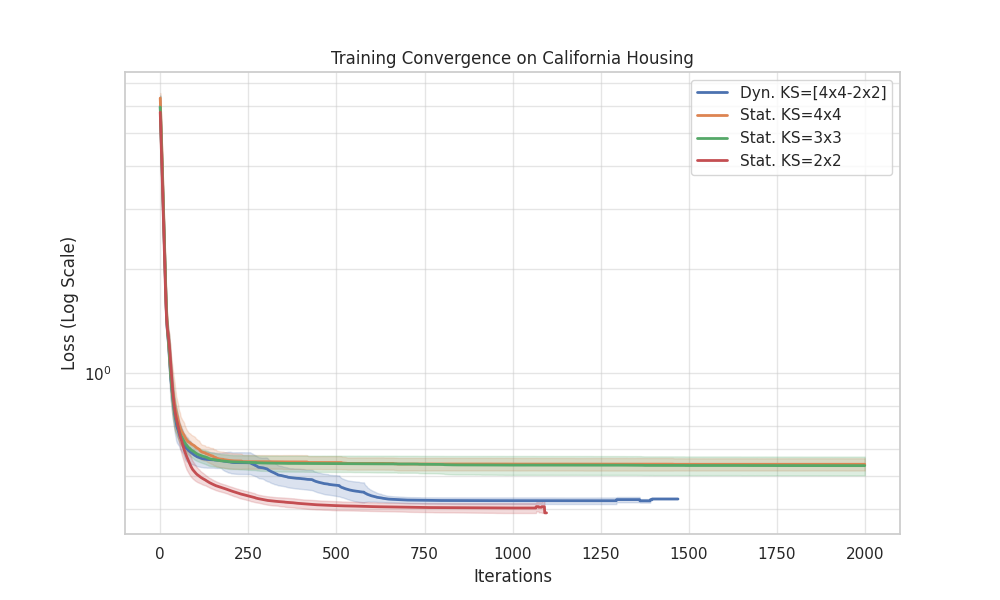
\includegraphics[width=0.9\textwidth]{figures/results/small_net_dynamic_kernels_reshaping/small_net_dynamic_kernels_reshaping_convergence.png}
    \caption{Training convergence comparison on a logarithmic scale.}
    \label{fig:small_net_convergence}
\end{figure}

The \textit{Dynamic} approach (blue line) demonstrates a superior ability to adapt compared to larger static kernels ($4 \times 4$ and $3 \times 3$), which plateau prematurely. The dynamic reshaping allows the network to "escape" these local minima, eventually settling into a performance range very close to the optimal $2 \times 2$ static configuration.

To assess the reliability of these results, Figure \ref{fig:small_net_final_loss} displays the distribution of the final loss values across the 5 independent runs.

\newpage

\begin{figure}[htbp]
    \centering
    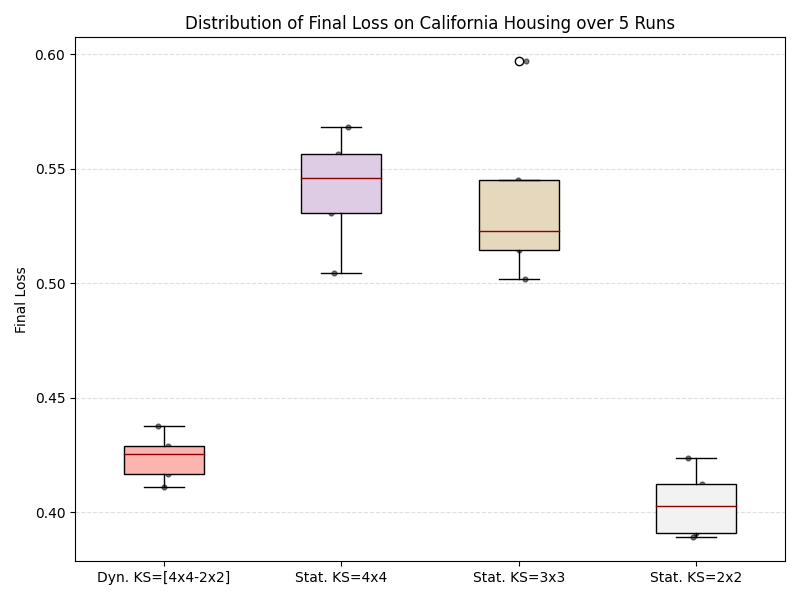
\includegraphics[width=0.85\textwidth]{figures/results/small_net_dynamic_kernels_reshaping/small_net_dynamic_kernels_reshaping_final_loss.png}
    \caption{Distribution of Final Loss over 5 runs.}
    \label{fig:small_net_final_loss}
\end{figure}

The boxplot highlights the stability of the \textit{Dynamic} method, which maintains a very tight distribution. In contrast, the static $3 \times 3$ and $4 \times 4$ kernels show not only higher average loss but also greater variance and presence of outliers, suggesting a higher sensitivity to weight initialization.

\newpage
Finally, we examine the broader predictive performance through the distribution of regression metrics (MSE, RMSE, MAE, and $R^2$), shown in Figure \ref{fig:small_net_metrics_dist}.

\begin{figure}[htbp]
    \centering
    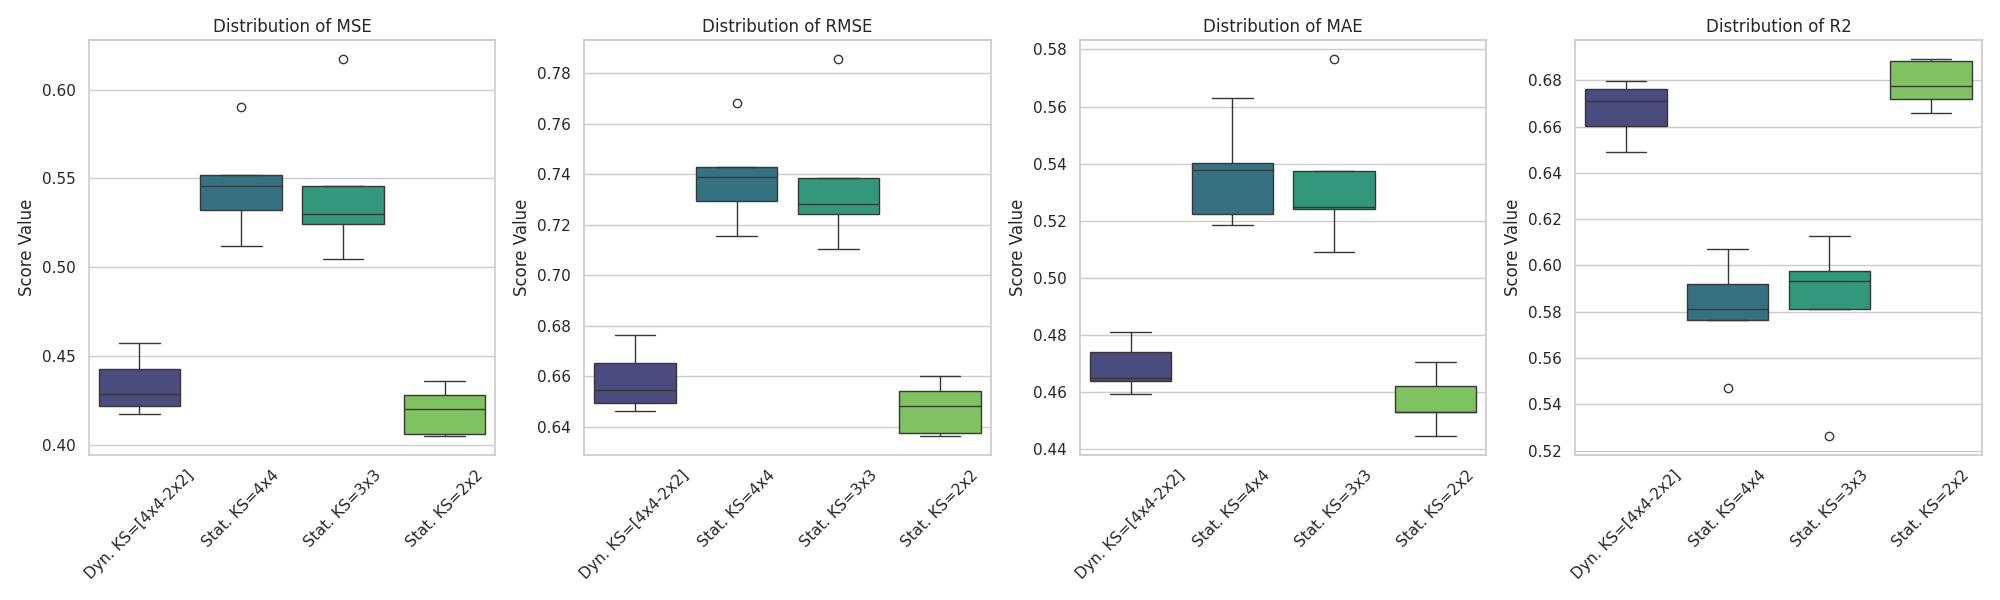
\includegraphics[width=1\textwidth]{figures/results/small_net_dynamic_kernels_reshaping/small_net_dynamic_kernels_reshaping_metrics_distribution.png}
    \caption{Boxplots for MSE, RMSE, MAE, and $R^2$ across all tested configurations.}
    \label{fig:small_net_metrics_dist}
\end{figure}

The metrics confirm that the Dynamic approach consistently matches or exceeds the performance of large static kernels across all indicators. Notably, the $R^2$ distribution for the dynamic method is centered around $0.67$, proving that it can autonomously find a near-optimal configuration for the California Housing task.

\subsubsection{Summary Statistics}

The numerical data summarized in Table \ref{tab:small_net_results} provides the final confirmation of these observations, illustrating the average performance across all metrics.

\begin{table}[h]
\centering
\scriptsize
\begin{tabular}{|l|c|c|c|c|}
\hline
\textbf{Metric (Avg)} & \textbf{Dynamic [4x4-2x2]} & \textbf{Static 4x4} & \textbf{Static 3x3} & \textbf{Static 2x2} \\ \hline
Final Loss            & 0.4239                     & 0.5411                & 0.5362                & 0.4036                \\ \hline
Time (s)              & 736.10                     & 387.30                & 527.97                & 721.80                \\ \hline
MSE                   & 0.4337                     & 0.5464                & 0.5444                & 0.4190                \\ \hline
RMSE                  & 0.6585                     & 0.7390                & 0.7374                & 0.6473                \\ \hline
MAE                   & 0.4686                     & 0.5363                & 0.5344                & 0.4567                \\ \hline
$R^2$                 & 0.6673                     & 0.5808                & 0.5823                & 0.6785                \\ \hline
\end{tabular}
\caption{Average performance summary for Small Net.}
\label{tab:small_net_results}
\end{table}


\newpage

\subsection{Medium Net Results}
The configuration parameters for the dynamic and static tests are outlined here:
\begin{itemize}
    \item \textbf{Weight Kernel Size:} Max $[6,6]$, Min $[2,2]$ (decrement: 1).
    \item \textbf{Bias Kernel Size:} Max $[6]$, Min $[2]$ (decrement: 1).
    \item \textbf{Strides:} Max 6, Min 2.
    \item \textbf{Runs:} 5 for each configuration.
\end{itemize}

\subsubsection{Visual Analysis of Training and Stability}

As illustrated in Figure \ref{fig:medium_net_convergence}, the training trajectory for the Medium Net shows a clear advantage for the dynamic approach. While large static kernels ($6 \times 6$ and $5 \times 5$) suffer from significant plateaus early in the training, the dynamic reshaping allows the model to continuously refine its representation.

\begin{figure}[htbp]
    \centering
    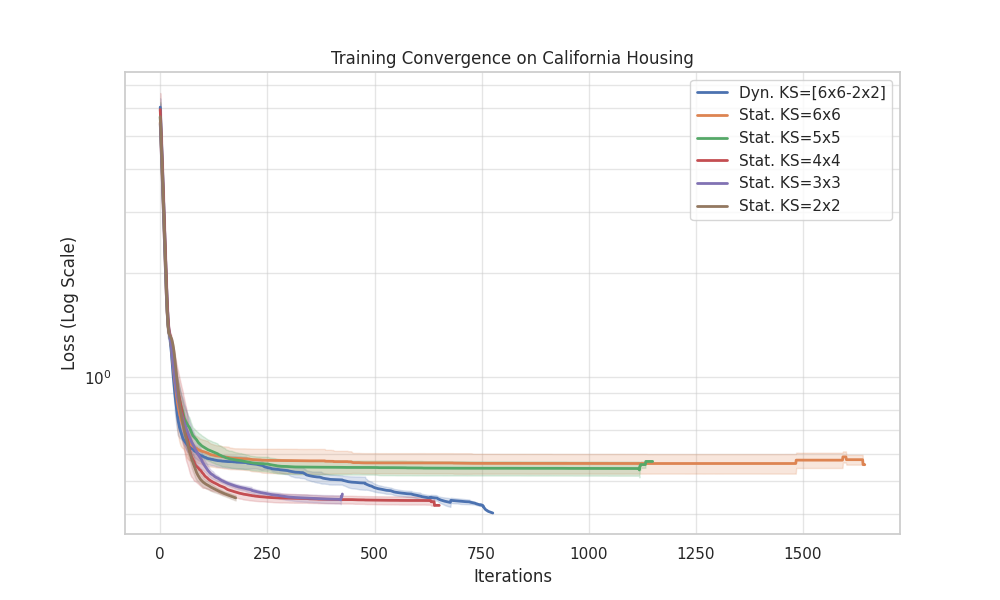
\includegraphics[width=0.9\textwidth]{figures/results/medium_net_dynamic_kernels_reshaping/medium_net_dynamic_kernels_reshaping_convergence.png}
    \caption{Training convergence comparison for the Medium Net on a logarithmic scale.}
    \label{fig:medium_net_convergence}
\end{figure}

The \textit{Dynamic} approach (blue line) begins to diverge from the suboptimal larger kernels after approximately 150 iterations, eventually achieving a lower final loss than even the best-performing static configurations ($4 \times 4$ and $3 \times 3$).

\newpage

To assess the reliability of these results, Figure \ref{fig:medium_net_final_loss} displays the distribution of the final loss values across the 5 independent runs.

\begin{figure}[htbp]
    \centering
    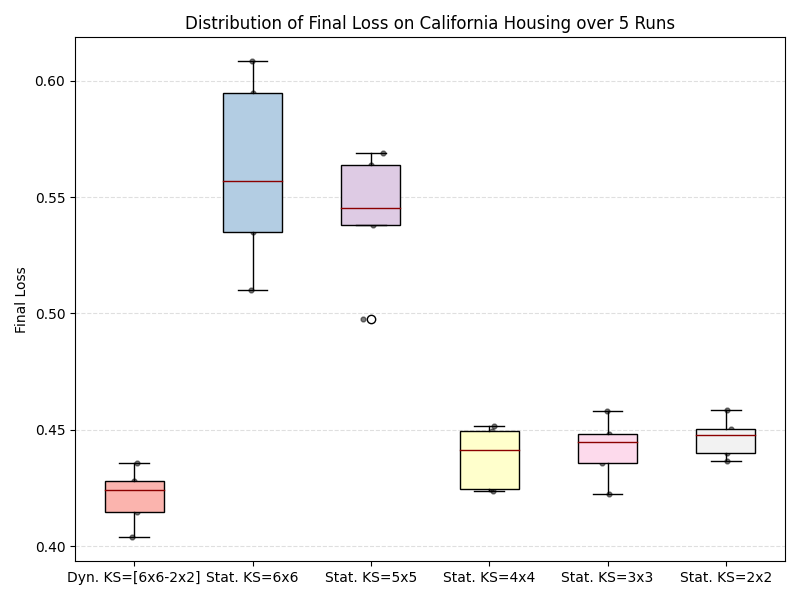
\includegraphics[width=0.85\textwidth]{figures/results/medium_net_dynamic_kernels_reshaping/medium_net_dynamic_kernels_reshaping_final_loss.png}
    \caption{Distribution of Final Loss over 5 runs for the Medium Net.}
    \label{fig:medium_net_final_loss}
\end{figure}

The boxplot confirms that the \textit{Dynamic} method is the most stable and effective configuration for this architecture. It exhibits the lowest median loss and a remarkably tight distribution, whereas the larger static kernels ($6 \times 6$ and $5 \times 5$) show both poor performance and higher variance.

\newpage

Finally, we examine the broader predictive performance through the distribution of regression metrics (MSE, RMSE, MAE, and $R^2$), shown in Figure \ref{fig:medium_net_metrics_dist}.

\begin{figure}[htbp]
    \centering
    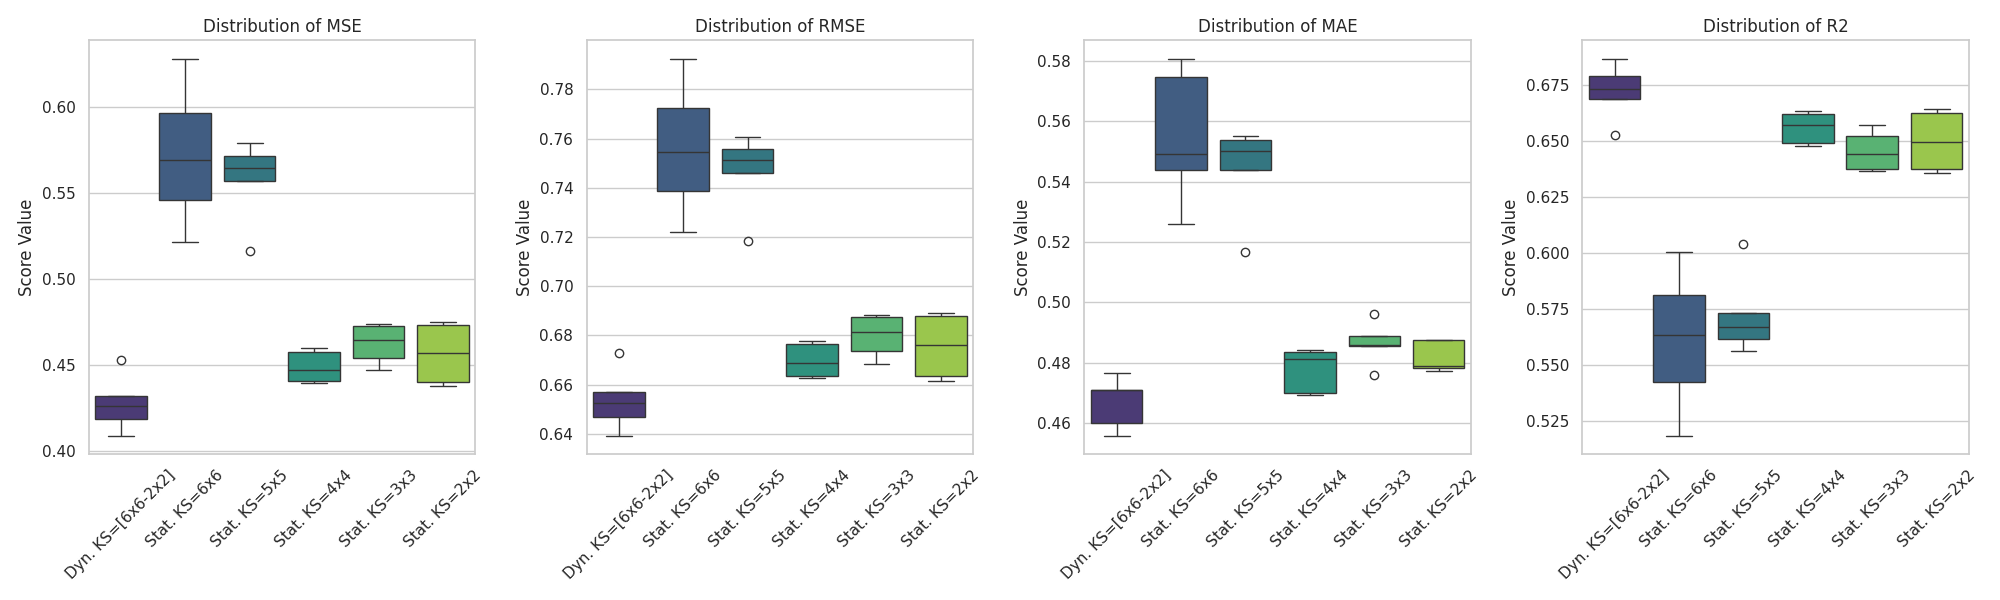
\includegraphics[width=1\textwidth]{figures/results/medium_net_dynamic_kernels_reshaping/medium_net_dynamic_kernels_reshaping_metrics_distribution.png}
    \caption{Boxplots for MSE, RMSE, MAE, and $R^2$ across all Medium Net configurations.}
    \label{fig:medium_net_metrics_dist}
\end{figure}

The metrics highlight a critical finding: for the Medium Net, the Dynamic approach consistently outperforms all static kernels across every indicator. Notably, the $R^2$ distribution for the dynamic method is centered above $0.67$, while all static configurations, including the previously optimal smaller kernels, fail to reach the same level of predictive accuracy.

\subsubsection{Summary Statistics}

The numerical data in Table \ref{tab:medium_net_results} provides the final confirmation. The Dynamic approach achieves the best average $R^2$ ($0.6720$) and the lowest average MSE ($0.4275$), proving its superiority in more complex architectures.

\begin{table}[h]
\centering
\scriptsize
\begin{tabular}{|l|c|c|c|c|c|c|}
\hline
\textbf{Metric (Avg)} & \textbf{Dyn. [6x6-2x2]} & \textbf{Stat. 6x6} & \textbf{Stat. 5x5} & \textbf{Stat. 4x4} & \textbf{Stat. 3x3} & \textbf{Stat. 2x2} \\ \hline
Final Loss            & 0.4212                  & 0.5610             & 0.5427             & 0.4382             & 0.4419             & 0.4467             \\ \hline
Time (s)              & 810.86                  & 745.08             & 745.80             & 751.14             & 758.06             & 756.91             \\ \hline
MSE                   & 0.4275                  & 0.5720             & 0.5574             & 0.4487             & 0.4622             & 0.4565             \\ \hline
RMSE                  & 0.6537                  & 0.7559             & 0.7465             & 0.6698             & 0.6798             & 0.6756             \\ \hline
MAE                   & 0.4670                  & 0.5549             & 0.5440             & 0.4777             & 0.4866             & 0.4820             \\ \hline
$R^2$                 & 0.6720                  & 0.5611             & 0.5723             & 0.6557             & 0.6454             & 0.6497             \\ \hline
\end{tabular}
\caption{Average performance summary for the Medium Net architecture.}
\label{tab:medium_net_results}
\end{table}

\newpage

\subsection{Big Net Results}

The Big Net architecture represents the most complex scenario, evaluated with the following setup:
\begin{itemize}
    \item \textbf{Weight Kernel Size:} Max $[8,8]$, Min $[3,3]$ (decrement: 1).
    \item \textbf{Bias Kernel Size:} Max $[8]$, Min $[3]$ (decrement: 1).
    \item \textbf{Strides:} Max 8, Min 3.
    \item \textbf{Runs:} 5 for each configuration.
\end{itemize}

\subsubsection{Visual Analysis of Training and Stability}

The training trajectory for the Big Net, shown in Figure \ref{fig:big_net_convergence}, illustrates the difficulty of optimizing larger architectures. We observe a significant failure in the \textit{Static 3x3} configuration, which remains trapped in a high-loss state.

\begin{figure}[htbp]
    \centering
    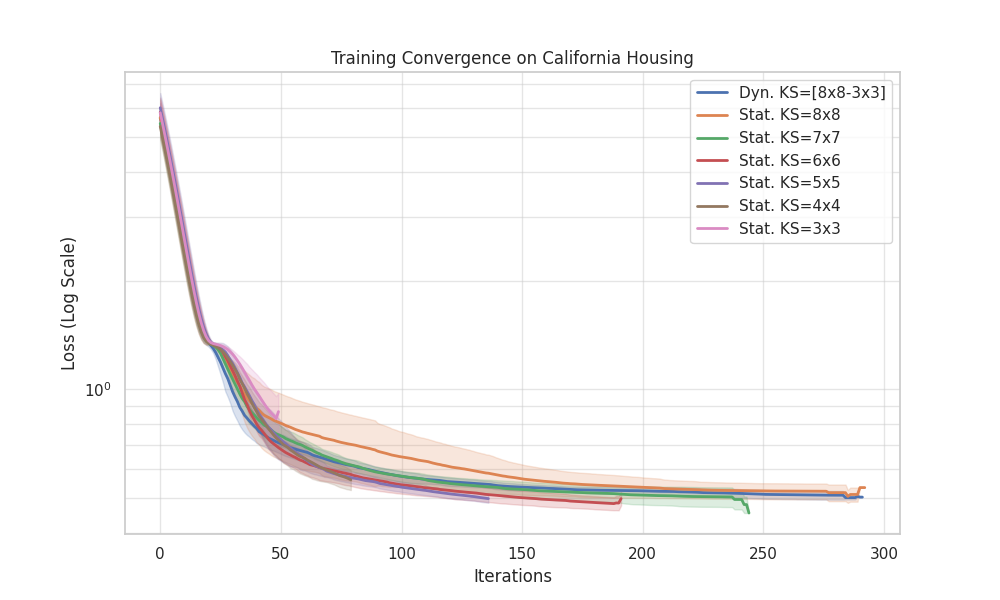
\includegraphics[width=0.9\textwidth]{figures/results/big_net_dynamic_kernels_reshaping/big_net_dynamic_kernels_reshaping_convergence.png}
    \caption{Training convergence comparison for the Big Net on a logarithmic scale.}
    \label{fig:big_net_convergence}
\end{figure}

The \textit{Dynamic} approach (blue line) successfully avoids the initialization issues that plague the smallest static kernels. It follows a stable descent path, mirroring the behavior of the most effective static kernels ($6 \times 6$ and $7 \times 7$), and proves that starting with a larger receptive field before reshaping is beneficial for deeper or wider networks.

Figure \ref{fig:big_net_final_loss} highlights the distribution of final loss values, providing insights into the robustness of each method.

\begin{figure}[htbp]
    \centering
    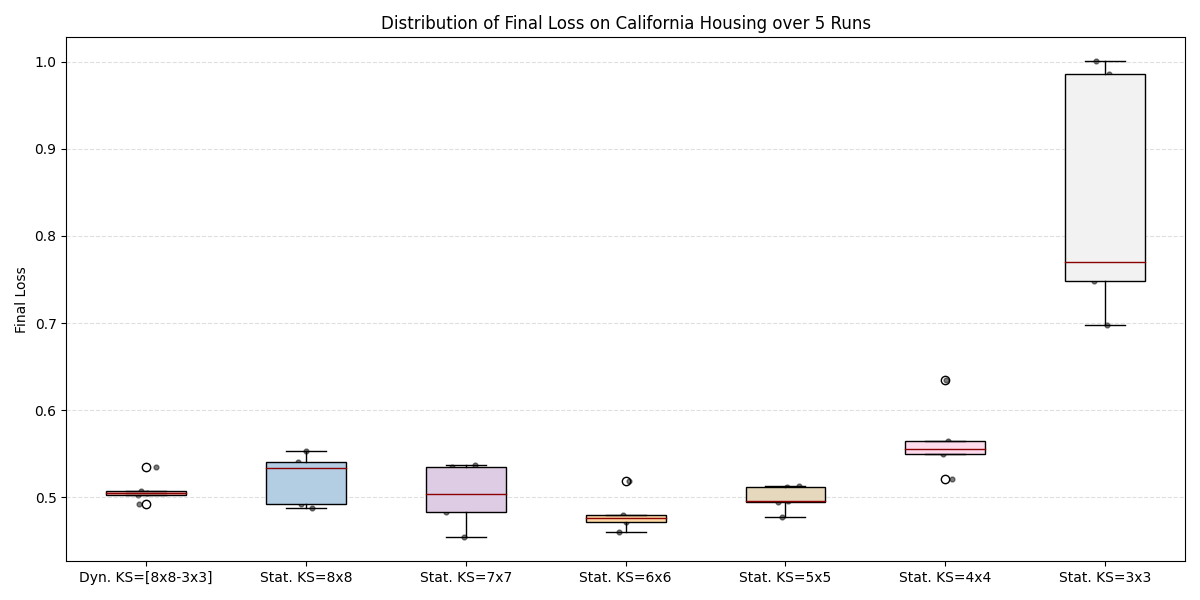
\includegraphics[width=0.85\textwidth]{figures/results/big_net_dynamic_kernels_reshaping/big_net_dynamic_kernels_reshaping_final_loss.png}
    \caption{Distribution of Final Loss over 5 runs for the Big Net.}
    \label{fig:big_net_final_loss}
\end{figure}

The boxplot clearly shows the catastrophic variance of the \textit{Static 3x3} configuration. In contrast, the \textit{Dynamic} method remains extremely stable. Although the \textit{Static 6x6} achieved the absolute lowest median loss in this specific test, the Dynamic approach provides a nearly identical performance level without any manual tuning, acting as a reliable "safety net" against suboptimal kernel choices.

\newpage

The broader predictive performance across regression metrics is presented in Figure \ref{fig:big_net_metrics_dist}.

\begin{figure}[htbp]
    \centering
    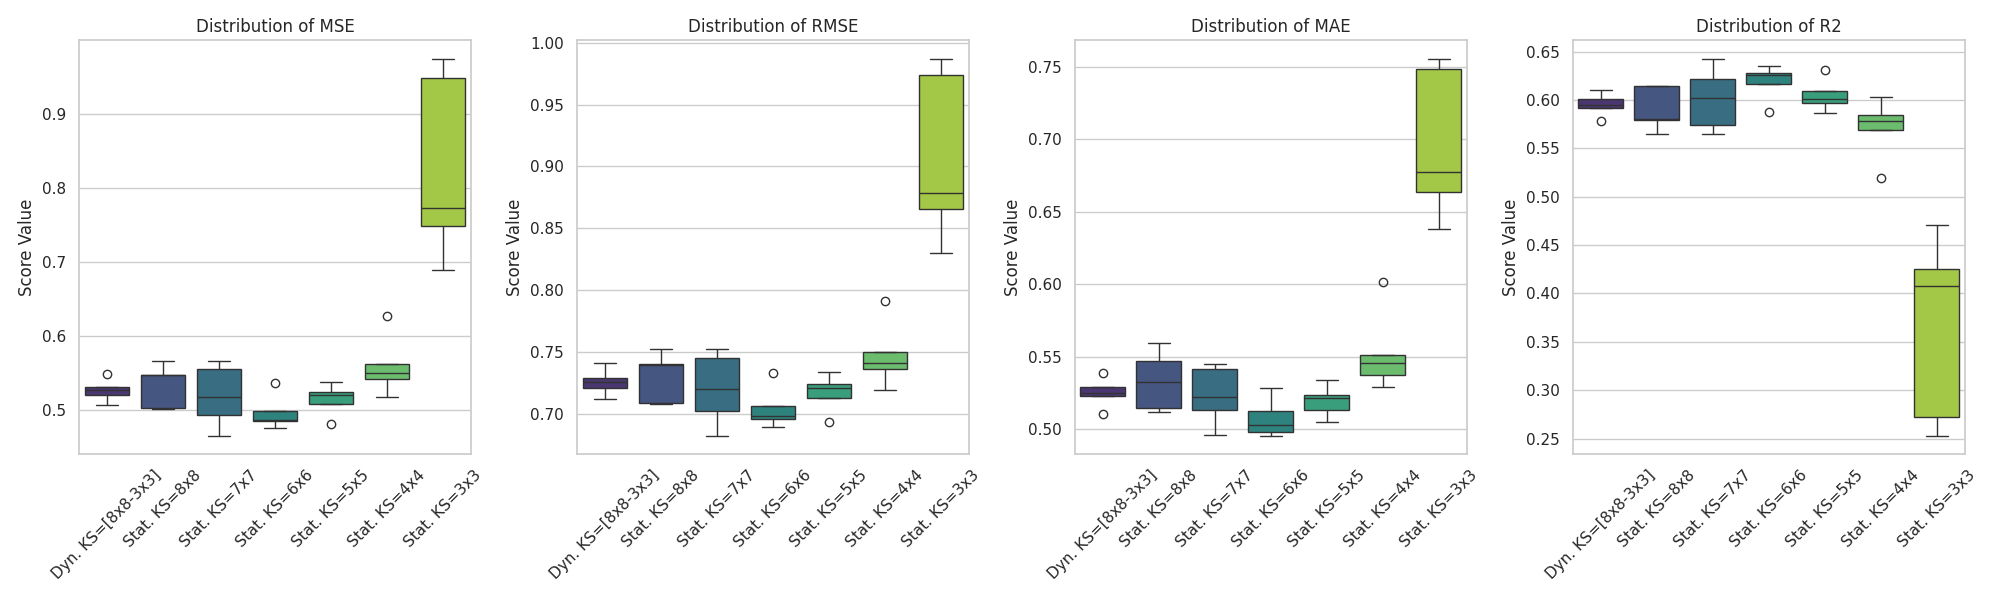
\includegraphics[width=1\textwidth]{figures/results/big_net_dynamic_kernels_reshaping/big_net_dynamic_kernels_reshaping_metrics_distribution.png}
    \caption{Boxplots for MSE, RMSE, MAE, and $R^2$ across all Big Net configurations.}
    \label{fig:big_net_metrics_dist}
\end{figure}

These distributions confirm the general trend: the Dynamic approach matches the predictive power of the best static configurations (6x6 and 7x7). As seen in the $R^2$ plot, the dynamic method centers its performance around $0.60$, effectively outperforming the 8x8, 4x4, and 3x3 static setups.

\subsubsection{Summary Statistics}

Table \ref{tab:big_net_results} summarizes the average metrics for the Big Net. The results prove that dynamic reshaping is a viable strategy for large networks, offering a balanced trade-off between execution time and predictive accuracy.

\begin{table}[h]
\centering
\resizebox{\textwidth}{!}{ % Inizia il ridimensionamento
\begin{tabular}{|l|c|c|c|c|c|c|c|}
\hline
\textbf{Metric (Avg)} & \textbf{Dyn. [8x-3x]} & \textbf{Stat. 8x8} & \textbf{Stat. 7x7} & \textbf{Stat. 6x6} & \textbf{Stat. 5x5} & \textbf{Stat. 4x4} & \textbf{Stat. 3x3} \\ \hline
Final Loss            & 0.5083                & 0.5214             & 0.5025             & 0.4813             & 0.4985             & 0.5652             & 0.8406             \\ \hline
Time (s)              & 704.31                & 708.07             & 716.08             & 712.44             & 702.59             & 698.35             & 696.42             \\ \hline
MSE                   & 0.5274                & 0.5335             & 0.5201             & 0.4972             & 0.5149             & 0.5600             & 0.8263             \\ \hline
RMSE                  & 0.7262                & 0.7302             & 0.7207             & 0.7050             & 0.7174             & 0.7479             & 0.9069             \\ \hline
MAE                   & 0.5252                & 0.5333             & 0.5236             & 0.5075             & 0.5196             & 0.5530             & 0.6964             \\ \hline
$R^2$                 & 0.5954                & 0.5907             & 0.6010             & 0.6185             & 0.6050             & 0.5705             & 0.3660             \\ \hline
\end{tabular}
} % Chiude il ridimensionamento
\caption{Average performance summary for the Big Net architecture.}
\label{tab:big_net_results}
\end{table}

\newpage

\subsection{Final Considerations on Dynamic Kernel Reshaping}

The comparative analysis across Small, Medium, and Big architectures allows for a comprehensive evaluation of the Dynamic Kernel Reshaping approach. The experimental results lead to several key conclusions regarding its performance, stability, and practical utility.

\subsubsection{Performance and Adaptability}
The primary objective was to determine if a dynamic approach could match or exceed the performance of statically defined kernels. The data suggests a nuanced but positive outcome:
\begin{itemize}
    \item \textbf{Near-Optimal Performance:} In the Small Net, the dynamic approach \\
    achieved results nearly identical to the best static configuration ($2 \times 2$), effectively closing the gap after a brief adaptation period.
    \item \textbf{Architectural Superiority:} In the Medium Net, the dynamic method \\
    demonstrated its maximum potential by \textit{outperforming all static configurations}. \\
    This suggests that as network complexity increases, the ability to adapt the receptive field during training becomes a significant competitive advantage.
    \item \textbf{Robustness in Large Scales:} For the Big Net, while the numerical results were comparable to the best-performing static kernels ($6 \times 6$), the dynamic approach proved essential in avoiding the catastrophic convergence failures observed with smaller static kernels ($3 \times 3$), which were unable to handle the increased depth of the architecture.
\end{itemize}

\subsubsection{Operational Efficiency and Parameter Tuning}
As hypothesized, the most significant practical benefit of Dynamic Kernel Reshaping is the elimination of exhaustive hyperparameter searches. Selecting the optimal kernel size is typically a trial-and-error process that varies significantly with network depth and task complexity. 

The dynamic schema acts as an automated optimizer: by starting with a larger receptive field to favor global feature exploration and gradually shrinking to smaller dimensions for fine-tuning, the model autonomously navigates toward a high-perfor\-mance state.


%%%%%%%%%%%%%%%% DYNAMIC QUANTIZATION FACTOR %%%%%%%%%%%%%%%%%%%%%%%

\section{Dynamic Quantization Factor Results}

This section investigates the impact of dynamically adjusting the quantization factor during the training process. The primary hypothesis is that increasing the quantization resolution when the loss improvement stalls can allow the $A^*$ algorithm to perform finer weight adjustments, potentially escaping local minima or refining the solution quality.

The dynamic approach is compared against several static quantization factors ($QF \in \{10^1, 10^2, 10^3, 10^4\}$) to evaluate whether an adaptive strategy can achieve the high precision of a large $QF$ without the computational search burden or the convergence difficulties often associated with high-resolution discrete spaces.

\subsection{Small Net Results}

For the Small Net architecture, the following parameters were utilized to establish the baseline and dynamic behavior:

\begin{itemize}
    \item \textbf{Weight Kernel Size:} $[2,2]$ (Static).
    \item \textbf{Bias Kernel Size:} $[2]$ (Static).
    \item \textbf{Strides:} 2.
    \item \textbf{Dynamic QF Range:} Min $10$, Max $10,000$ (Multiplier: 10).
    \item \textbf{Runs:} 5 for each configuration.
\end{itemize}

\newpage

\subsubsection{Visual Analysis of Training and Stability}

The convergence behavior, as depicted in Figure \ref{fig:small_net_quant_convergence}, reveals a stark contrast between low and high quantization factors. Low static factors ($10^1$ and $10^2$) lead to rapid initial convergence. In contrast, static factors of $10^3$ and $10^4$ struggle significantly, failing to achieve a competitive loss within the same iteration limit.

\begin{figure}[htbp]
    \centering
    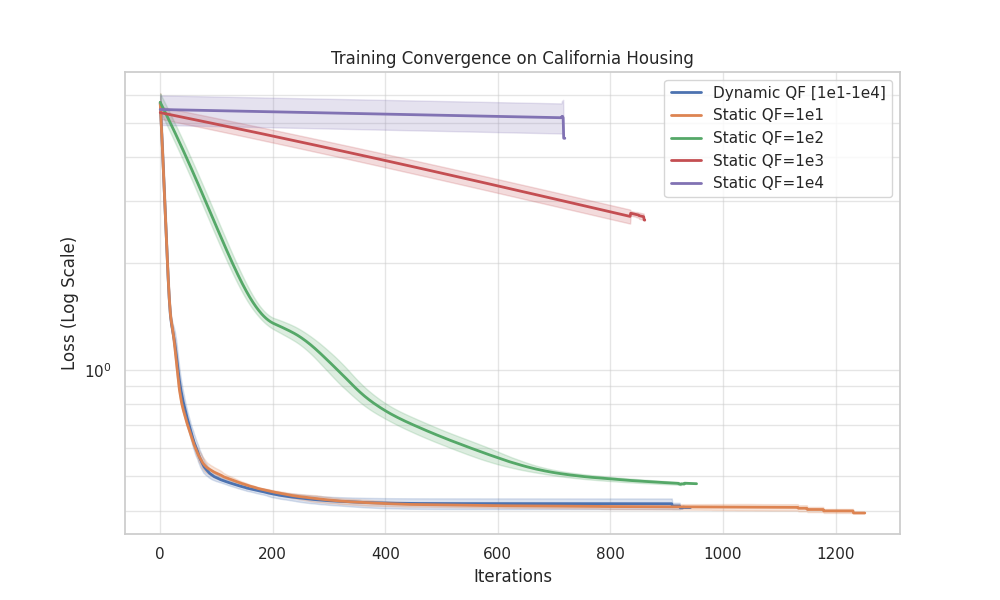
\includegraphics[width=0.9\textwidth]{figures/results/small_net_dynamic_quantization_factor/small_net_dynamic_quantization_factor_convergence.png}
    \caption{Training convergence comparison for various Quantization Factors (Log Scale).}
    \label{fig:small_net_quant_convergence}
\end{figure}

The \textit{Dynamic QF} strategy (blue line) successfully mirrors the rapid descent of the $QF=10$ configuration. This suggests that starting with a lower resolution allows for broad, efficient exploration of the weight space, while the dynamic increases (triggered by stalls) ensure the model maintains progress.

\newpage

Figure \ref{fig:small_net_quant_final_loss} illustrates the distribution of the final loss. The Dynamic QF approach demonstrates high stability, with a median loss of approximately $0.41$, nearly identical to the best-performing static model ($QF=10$).

\begin{figure}[htbp]
    \centering
    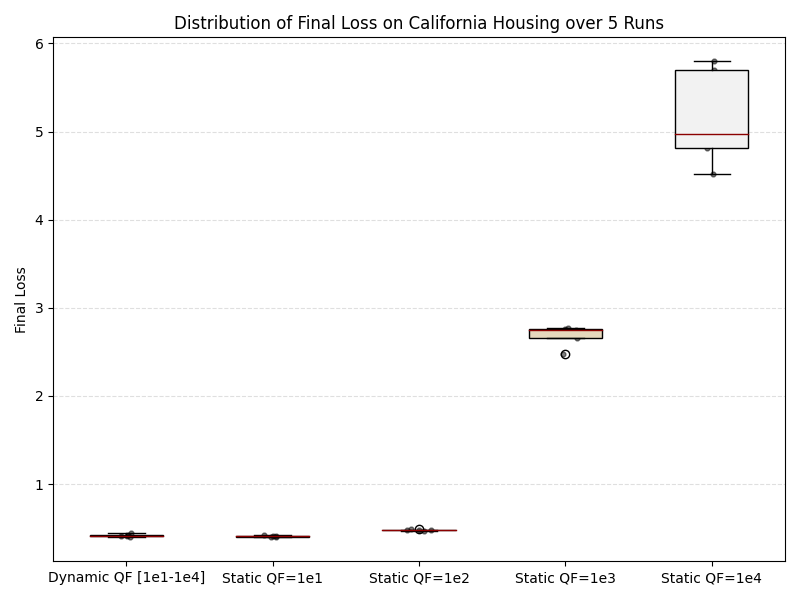
\includegraphics[width=0.85\textwidth]{figures/results/small_net_dynamic_quantization_factor/small_net_dynamic_quantization_factor_final_loss.png}
    \caption{Distribution of Final Loss over 5 runs for Quantization Factor tests.}
    \label{fig:small_net_quant_final_loss}
\end{figure}

As the static quantization factor increases beyond $10^2$, we observe not only a higher average loss but also a significant increase in variance. This confirms that excessively high quantization at the start of training makes the search landscape too complex for the algorithm to navigate effectively.

\newpage
The regression metrics across the 5 runs are summarized in Figure \ref{fig:small_net_quant_metrics_dist}.

\begin{figure}[htbp]
    \centering
    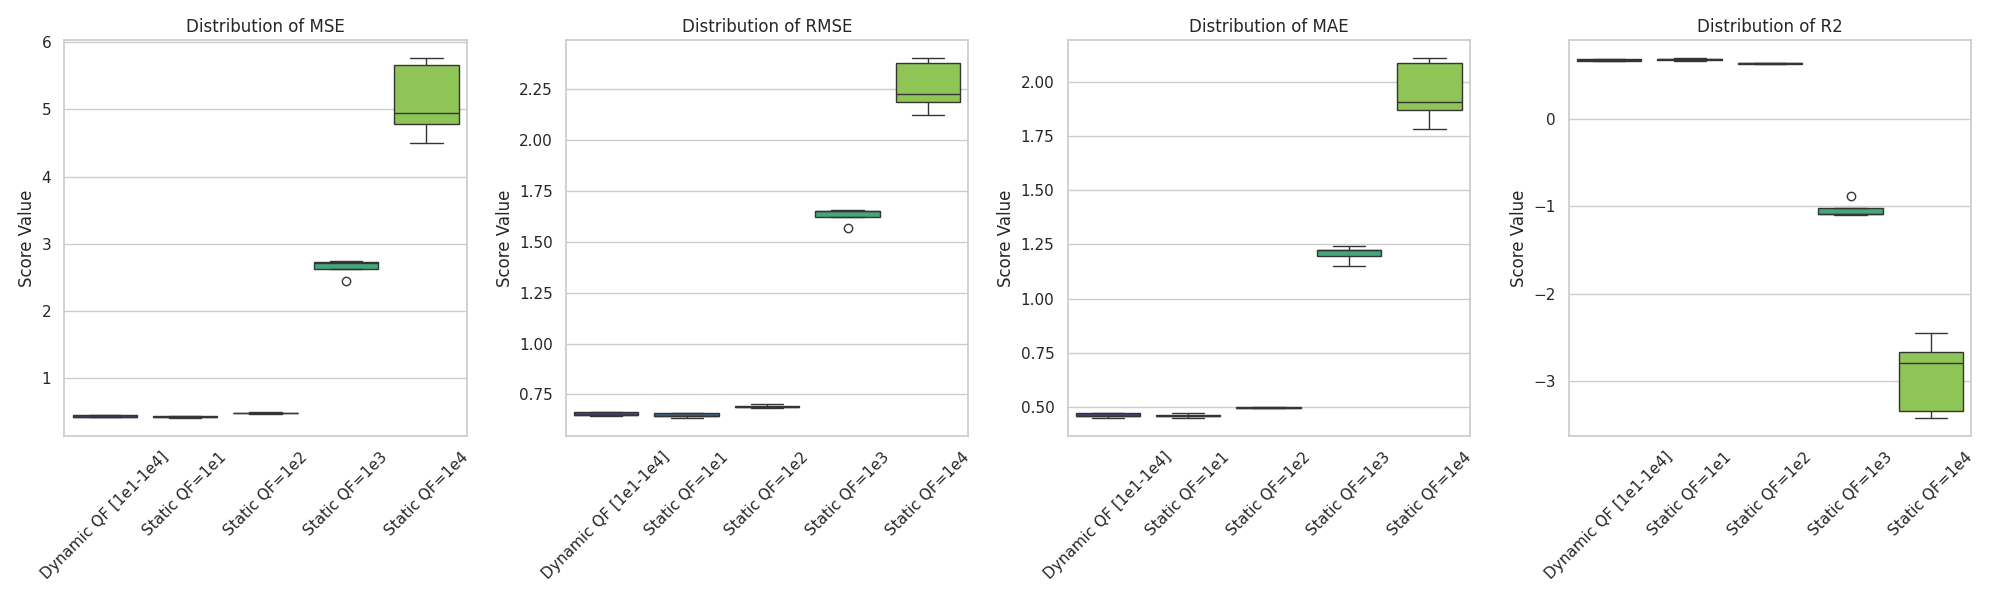
\includegraphics[width=1\textwidth]{figures/results/small_net_dynamic_quantization_factor/small_net_dynamic_quantization_factor_metrics_distribution.png}
    \caption{Regression metrics distribution (MSE, RMSE, MAE, and $R^2$) for Quantization Factor configurations.}
    \label{fig:small_net_quant_metrics_dist}
\end{figure}

The metrics highlight that the \textit{Dynamic QF} and \textit{Static QF=10, 100} are the only configurations achieving a positive and high $R^2$ score (approximately $0.67$). For static factors of $10^3$ and $10^4$, the $R^2$ values become negative, indicating that the models perform worse than a horizontal baseline, further justifying the need for a dynamic or low-starting quantization approach.

\subsubsection{Summary Statistics}

The average values for all metrics, compiled in Table \ref{tab:small_net_quant_results}, provide a definitive comparison of the performance levels.

\begin{table}[h]
\centering
\scriptsize
\begin{tabular}{|l|c|c|c|c|c|}
\hline
\textbf{Metric (Avg)} & \textbf{Dynamic [1e1-1e4]} & \textbf{Static 1e1} & \textbf{Static 1e2} & \textbf{Static 1e3} & \textbf{Static 1e4} \\ \hline
Final Loss            & 0.4184                     & 0.4085               & 0.4770               & 2.6815               & 5.1592               \\ \hline
Time (s)              & 667.96                     & 777.83               & 644.30               & 579.98               & 492.87               \\ \hline
MSE                   & 0.4268                     & 0.4208               & 0.4788               & 2.6506               & 5.1290               \\ \hline
RMSE                  & 0.6532                     & 0.6486               & 0.6919               & 1.6277               & 2.2621               \\ \hline
MAE                   & 0.4634                     & 0.4618               & 0.4983               & 1.2077               & 1.9496               \\ \hline
$R^2$                 & 0.6725                     & 0.6772               & 0.6327               & -1.0336              & -2.9352              \\ \hline
\end{tabular}
\caption{Average performance summary for Small Net (Quantization Factor Study).}
\label{tab:small_net_quant_results}
\end{table}


\subsection{Medium Net Results}

The evaluation of the Dynamic Quantization Factor (QF) was extended to the Medium Net architecture to assess how increased model complexity interacts with search space resolution. The configuration remained consistent with the previous test to ensure comparability:

\begin{itemize}
    \item \textbf{Weight Kernel Size:} $[2,2]$ (Static).
    \item \textbf{Bias Kernel Size:} $[2]$ (Static).
    \item \textbf{Strides:} 2.
    \item \textbf{Dynamic QF Range:} Min $10$, Max $10,000$ (Multiplier: 10).
    \item \textbf{Runs:} 5 for each configuration.
\end{itemize}

\subsubsection{Visual Analysis of Training and Stability}

As shown in Figure \ref{fig:medium_net_quant_convergence}, the convergence trends for the Medium Net reinforce the observations from the Small Net but with more pronounced performance gaps. Static factors of $10^3$ and $10^4$ show almost no effective optimization, maintaining a high loss throughout the iterations.

\begin{figure}[htbp]
    \centering
    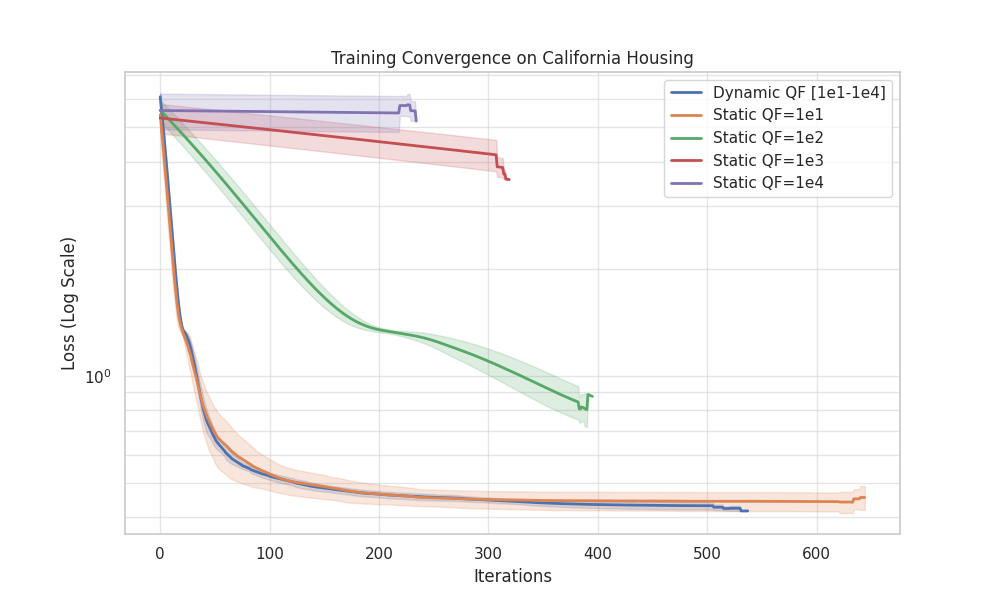
\includegraphics[width=0.9\textwidth]{figures/results/medium_net_dynamic_quantization_factor/medium_net_dynamic_quantization_factor_convergence.png}
    \caption{Training convergence comparison for Medium Net (Log Scale).}
    \label{fig:medium_net_quant_convergence}
\end{figure}

Interestingly, the \textit{Dynamic QF} strategy (blue line) demonstrates a highly efficient trajectory, converging rapidly and reaching a final loss state that is slightly lower than the $QF=10$ static baseline. This suggests that as the network grows in size, the ability to dynamically refine weight updates becomes increasingly valuable for fine-tuning.

Figure \ref{fig:medium_net_quant_final_loss} highlights the stability of these results. The Dynamic QF approach maintains a very low variance (Std: $0.0108$), outperforming the Static $QF=10$ in terms of consistency.


\begin{figure}[htbp]
    \centering
    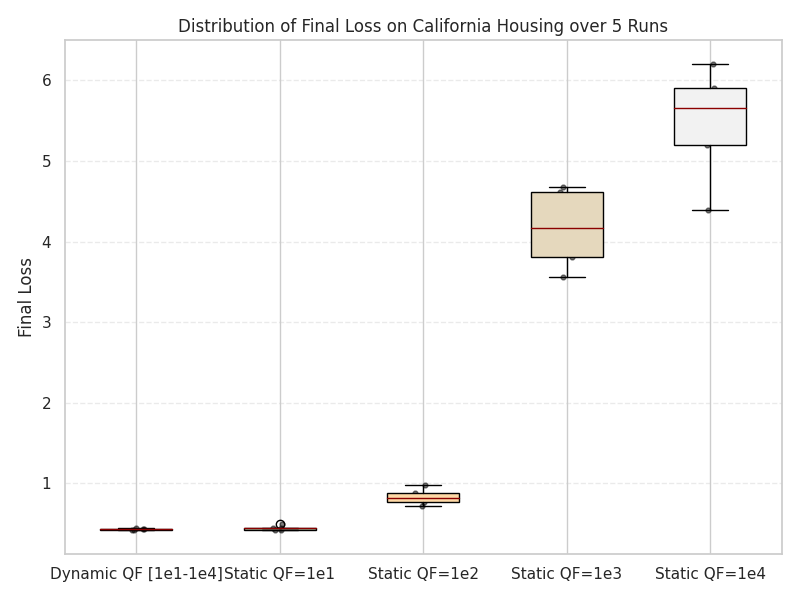
\includegraphics[width=0.85\textwidth]{figures/results/medium_net_dynamic_quantization_factor/medium_net_dynamic_quantization_factor_final_loss.png}
    \caption{Distribution of Final Loss for Medium Net configurations.}
    \label{fig:medium_net_quant_final_loss}
\end{figure}

A critical observation is the behavior of the Static $QF=10^2$ configuration. While it was somewhat competitive in the Small Net, its performance degrades significantly in the Medium Net (Avg Loss $0.83$ vs $0.47$ in Small Net). This indicates that higher-dimensional networks are more sensitive to initial discretization errors.

\newpage
The regression metrics for the Medium Net are visualized in Figure \ref{fig:medium_net_quant_metrics_dist}.

\begin{figure}[htbp]
    \centering
    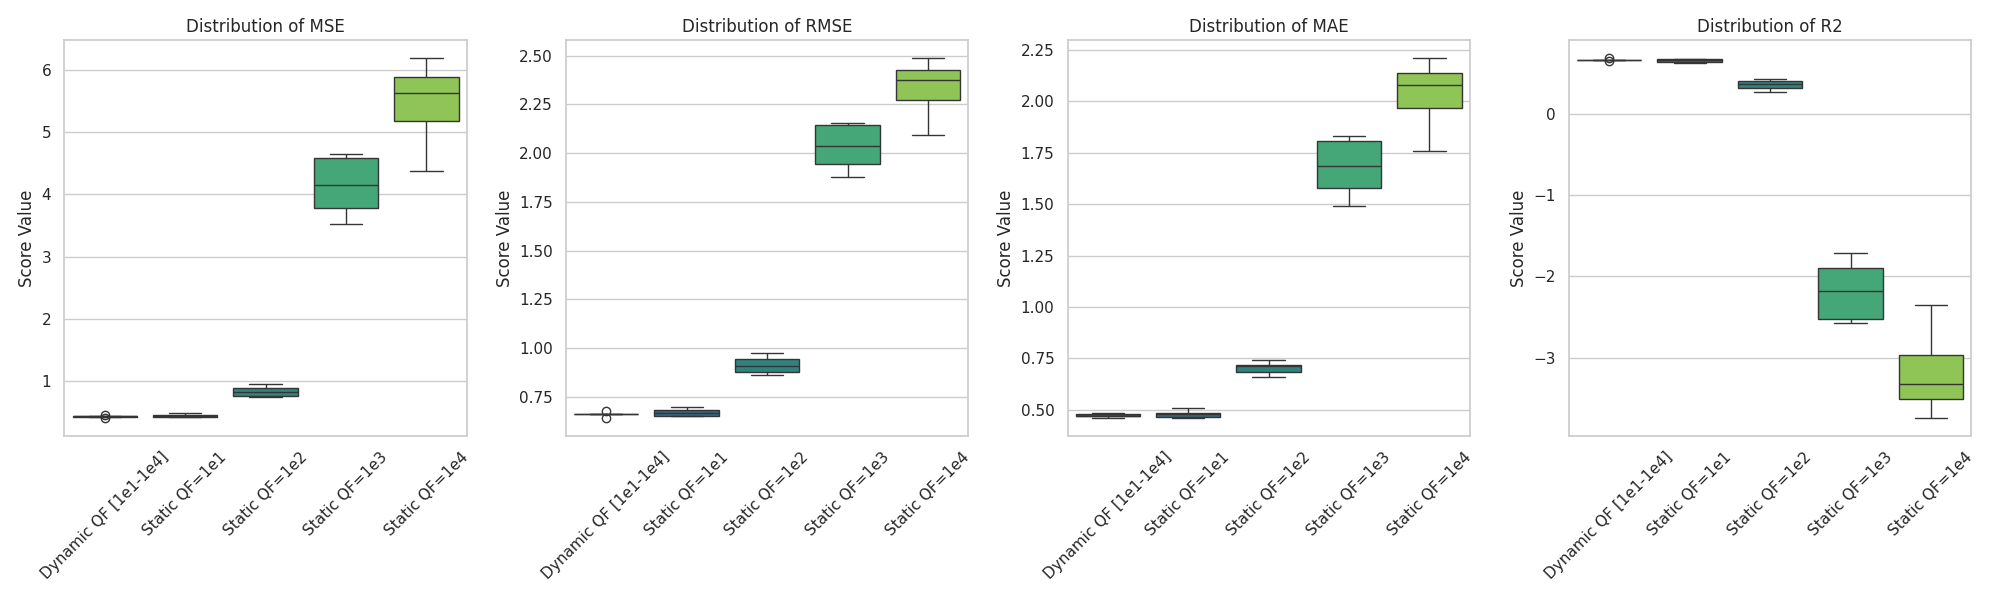
\includegraphics[width=1\textwidth]{figures/results/medium_net_dynamic_quantization_factor/medium_net_dynamic_quantization_factor_metrics_distribution.png}
    \caption{Regression metrics distribution for Medium Net configurations.}
    \label{fig:medium_net_quant_metrics_dist}
\end{figure}

The metrics confirm that the \textit{Dynamic QF} achieves the best overall performance, with an average $R^2$ of $0.6646$, slightly surpassing the $0.6535$ achieved by the Static $QF=10$. Configurations with $QF \geq 10^3$ fail to produce meaningful predictive models, as evidenced by the high MSE and negative $R^2$ values.

\subsubsection{Summary Statistics}

Table \ref{tab:medium_net_quant_results} provides the numerical breakdown of the average metrics for the Medium Net.

\begin{table}[h]
\centering
\scriptsize
\begin{tabular}{|l|c|c|c|c|c|}
\hline
\textbf{Metric (Avg)} & \textbf{Dynamic [1e1-1e4]} & \textbf{Static 1e1} & \textbf{Static 1e2} & \textbf{Static 1e3} & \textbf{Static 1e4} \\ \hline
Final Loss            & 0.4308            & 0.4423               & 0.8327               & 4.1656               & 5.4733               \\ \hline
Time (s)              & 618.54            & 739.54               & 465.80               & 379.06               & 283.61               \\ \hline
MSE                   & 0.4371            & 0.4516               & 0.8373               & 4.1377               & 5.4457               \\ \hline
RMSE                  & 0.6611            & 0.6717               & 0.9140               & 2.0312               & 2.3295               \\ \hline
MAE                   & 0.4742            & 0.4794               & 0.7030               & 1.6773               & 2.0293               \\ \hline
$R^2$                 & 0.6646            & 0.6535               & 0.3576               & -2.1746              & -3.1782              \\ \hline
\end{tabular}
\caption{Average performance summary for Medium Net (Quantization Factor Study).}
\label{tab:medium_net_quant_results}
\end{table}

\subsection{Big Net Results}

Finally, the study concludes with the Big Net architecture. As the number of parameters increases, the search space becomes exponentially more complex, making the initial selection of a quantization factor a determining factor for training success. The experimental parameters remained as follows:

\begin{itemize}
    \item \textbf{Weight Kernel Size:} $[2,2]$ (Static).
    \item \textbf{Bias Kernel Size:} $[2]$ (Static).
    \item \textbf{Strides:} 2.
    \item \textbf{Dynamic QF Range:} Min $10$, Max $10,000$ (Multiplier: 10).
    \item \textbf{Runs:} 5 for each configuration.
\end{itemize}


\subsubsection{Visual Analysis of Training and Stability}

The convergence patterns for the Big Net, shown in Figure \ref{fig:big_net_quant_convergence}, demonstrate that the $A^*$ algorithm's efficiency is highly dependent on low-resolution starts for large architectures. Similar to previous networks, $QF=10^3$ and $QF=10^4$ are unable to achieve meaningful optimization, plateauing almost immediately.

\begin{figure}[htbp]
    \centering
    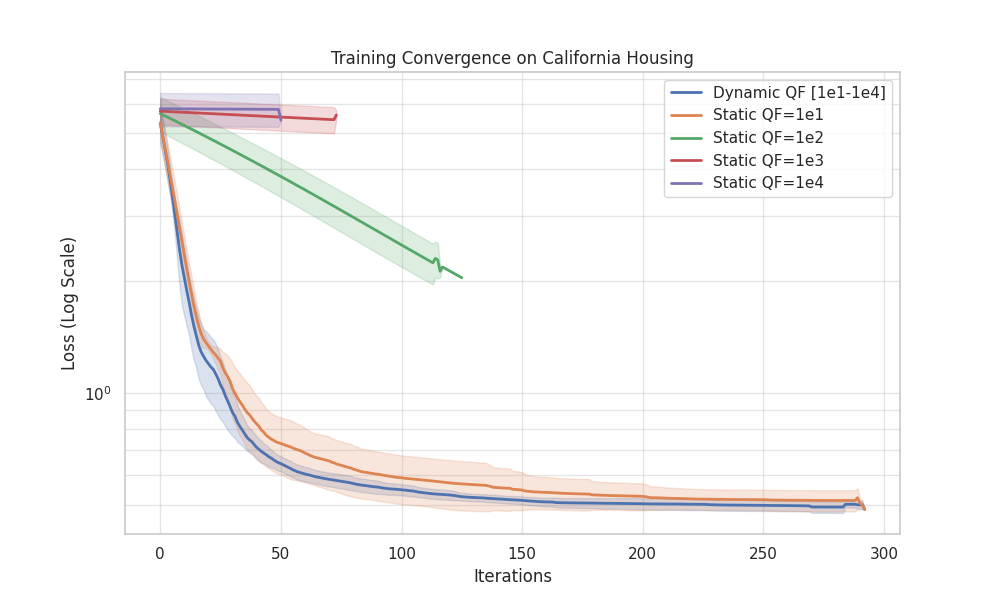
\includegraphics[width=0.9\textwidth]{figures/results/big_net_dynamic_quantization_factor/big_net_dynamic_quantization_factor_convergence.png}
    \caption{Training convergence comparison for Big Net (Log Scale).}
    \label{fig:big_net_quant_convergence}
\end{figure}

The \textit{Dynamic QF} strategy (blue line) exhibits a superior convergence rate even compared to the best static configuration ($QF=10$). In this high-dimensional setting, the dynamic approach proves to be the most robust, navigating the complex loss landscape more effectively than any fixed-resolution method.

Figure \ref{fig:big_net_quant_final_loss} confirms this superiority. Not only does the Dynamic QF achieve the lowest average loss, but it also demonstrates significantly lower variance compared to the $QF=10$ static run, which shows several higher-loss outliers.

\begin{figure}[htbp]
    \centering
    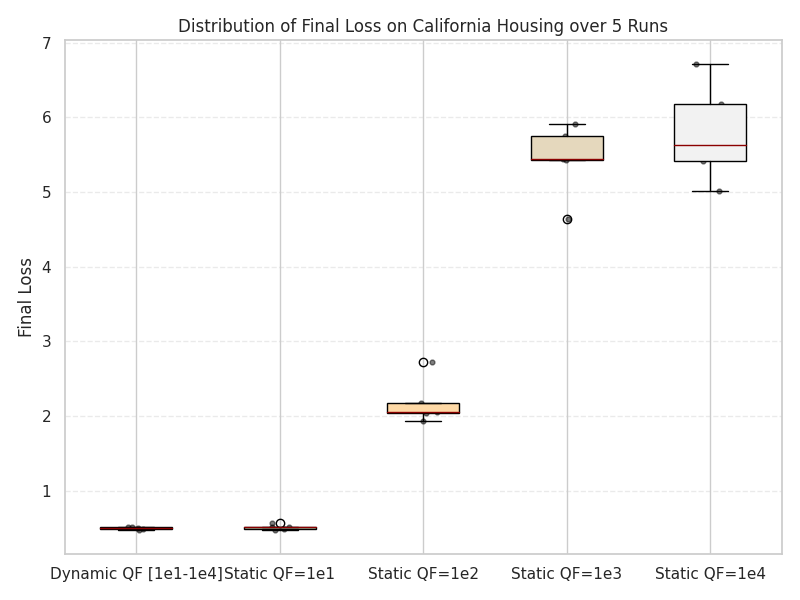
\includegraphics[width=0.85\textwidth]{figures/results/big_net_dynamic_quantization_factor/big_net_dynamic_quantization_factor_final_loss.png}
    \caption{Distribution of Final Loss for Big Net configurations.}
    \label{fig:big_net_quant_final_loss}
\end{figure}

The failure of the $QF=10^2$ configuration is even more evident here than in the Medium Net; while it manages a slow descent, its final loss (Avg 2.18) remains far from the optimal region, highlighting that higher parameter counts require even more careful discretization management.

\newpage
The comparative regression metrics are presented in Figure \ref{fig:big_net_quant_metrics_dist}.

\begin{figure}[htbp]
    \centering
    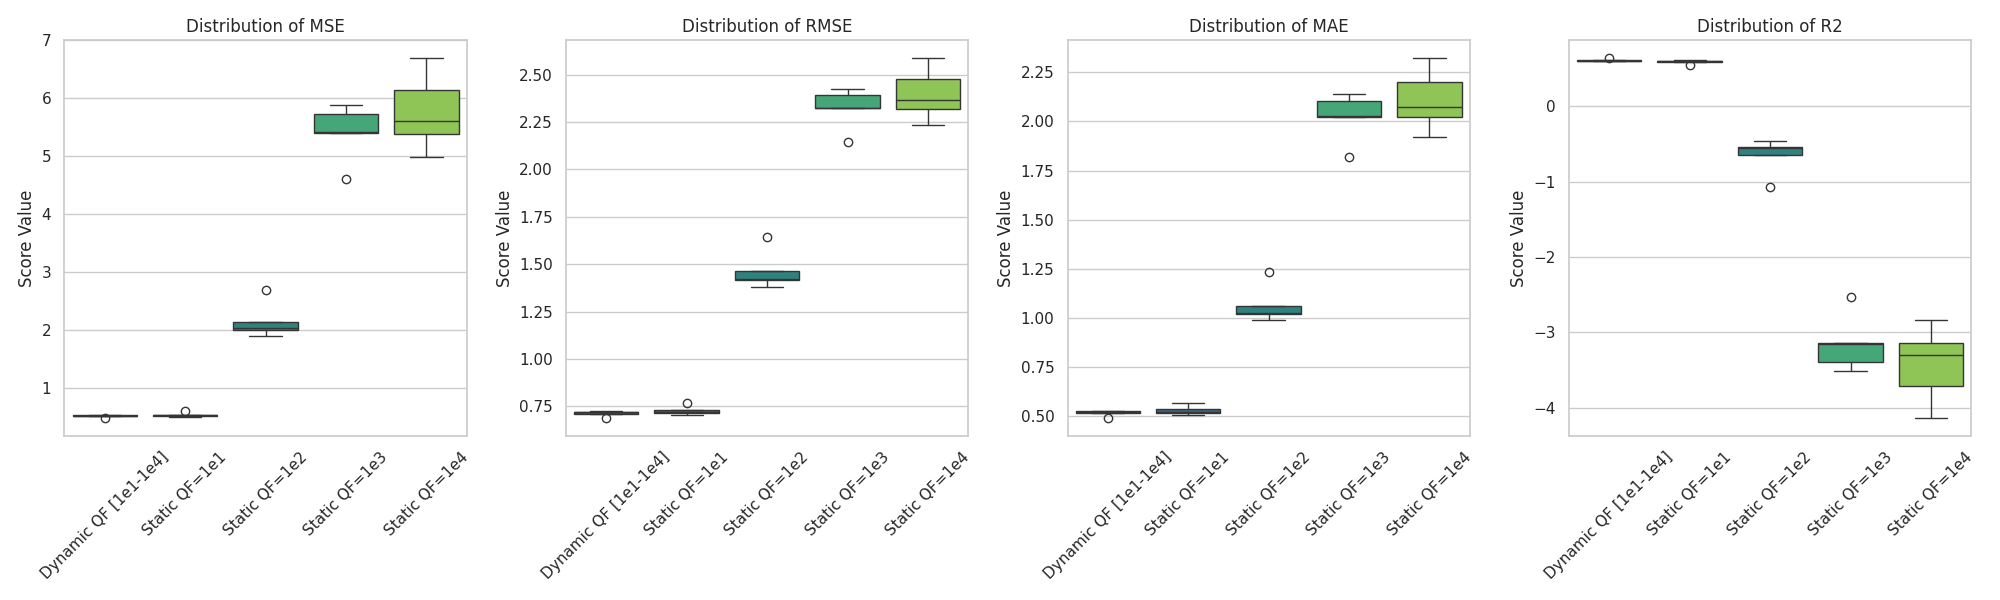
\includegraphics[width=1\textwidth]{figures/results/big_net_dynamic_quantization_factor/big_net_dynamic_quantization_factor_metrics_distribution.png}
    \caption{Regression metrics distribution for Big Net configurations.}
    \label{fig:big_net_quant_metrics_dist}
\end{figure}

The \textit{Dynamic QF} achieves an average $R^2$ of $0.6106$, outperforming the $0.5931$ of the static $QF=10$ case. The significant drop in $R^2$ for $QF=10^2$ (which becomes negative at $-0.65$) underscores the "discretization trap" where a slightly too-high resolution prevents the algorithm from finding the global descent direction in large models.

\subsubsection{Summary Statistics}

The numerical results for the Big Net are detailed in Table \ref{tab:big_net_quant_results}.

\begin{table}[h]
\centering
\scriptsize
\begin{tabular}{|l|c|c|c|c|c|}
\hline
\textbf{Metric (Avg)} & \textbf{Dynamic [1e1-1e4]} & \textbf{Static 1e1} & \textbf{Static 1e2} & \textbf{Static 1e3} & \textbf{Static 1e4} \\ \hline
Final Loss            & 0.4959            & 0.5133               & 2.1827               & 5.4331               & 5.7914               \\ \hline
Time (s)              & 703.85            & 716.39               & 300.36               & 190.66               & 135.31               \\ \hline
MSE                   & 0.5075            & 0.5303               & 2.1525               & 5.4062               & 5.7643               \\ \hline
RMSE                  & 0.7123            & 0.7279               & 1.4642               & 2.3231               & 2.3977               \\ \hline
MAE                   & 0.5146            & 0.5290               & 1.0635               & 2.0227               & 2.1074               \\ \hline
$R^2$                 & 0.6106            & 0.5931               & -0.6515              & -3.1478              & -3.4226              \\ \hline
\end{tabular}
\caption{Average performance summary for Big Net (Quantization Factor Study).}
\label{tab:big_net_quant_results}
\end{table}

\subsection{Conclusion on Dynamic Quantization Factor Study}

The experimental campaign across three architectures of increasing complexity — Small, Medium, and Big Net — provides a clear understanding of how the quantization factor ($QF$) influences the $A^*$ search space in neural network training.

\begin{itemize}
    \item \textbf{Robustness against the "Discretization Trap":} The most significant finding is that while low static quantization ($QF=10$) performs well, static factors from $10^2$ upwards lead to a rapid degradation of performance as the network size increases. The \textit{Dynamic QF} strategy effectively mitigates this risk by starting with a coarse resolution to find the global descent direction and only increasing precision when local stalls occur.
    
    \item \textbf{Performance Trends in Scalability:} For Medium and Big Net architectures, the \textit{Dynamic QF} approach did not only match but consistently \textbf{outperformed} the best static configurations in terms of final MSE and $R^2$ score. While the margin of improvement in the Small Net was negligible, the benefits became more pronounced as the parameter space expanded, suggesting that adaptive precision is a key requirement for scaling $A^*$-based training.
    
    \item \textbf{Operational Efficiency:} Beyond the raw metrics, the primary advantage of the dynamic approach is the \textbf{elimination of the hyperparameter search process}. Manually identifying the optimal $QF$ for a specific architecture is a computationally expensive trial-and-error task. The dynamic strategy offers a "set-and-forget" solution that guarantees near-optimal or superior performance across different network depths.
    
    \item \textbf{Convergence Stability:} As evidenced by the boxplots, the Dynamic QF approach significantly reduced the variance of the final loss compared to static methods. This stability is crucial for ensuring reliable training outcomes across multiple runs, regardless of weight initialization.
\end{itemize}

In conclusion, the \textbf{Dynamic Quantization Factor} is an essential optimization. It provides the algorithm with the flexibility to balance broad exploration with high-precision refinement, making the training process both more accurate and significantly more user-friendly by removing a critical hyperparameter from manual tuning.


%%%%%%%%%%%%%%%%%% SAMPLING PARAMETERS %%%%%%%%%%%%%%%%%%%%%%%%%%%%%%%%
\newpage

\section{Random Neighbors Generation: Grid Search on Sampling Parameters}
\label{sec:random_sampling_study}

This section explores the \textit{Random Neighbors Generation} strategy, which introduces a stochastic approach to weight optimization. Unlike the deterministic kernel-based methods, this scheme relies on two primary hyperparameters to define the search neighborhood: the \textit{Perturbation Ratio} and the \textit{Search Coverage Ratio}.

The \textit{Perturbation Ratio} determines the cardinality of the subset of parameters updated simultaneously within each layer. It is expressed as a percentage of the total number of parameters per layer ($|W_{layer}| \times \text{Perturbation Ratio}$). The \textit{Search Coverage Ratio} governs the total number of child nodes generated for each search step, similarly defined as a percentage of the total parameters in the layer. 

The objective of this grid search is to identify the optimal balance between the intensity of each update (perturbation) and the breadth of the local search (coverage) to maximize convergence efficiency in a discrete state-space.

\subsection{Small Net Results}

For the Small Net architecture, a grid search was conducted using the following parameter combinations:
\begin{itemize}
    \item \textbf{Perturbation Ratios:} $[0.01, 0.05, 0.1]$ ($1\%, 5\%, 10\%$).
    \item \textbf{Search Coverage Ratios:} $[0.05, 0.1, 0.2]$ ($5\%, 10\%, 20\%$).
    \item \textbf{Iterations:} 2000.
    \item \textbf{Runs:} 5 for each unique pair.
\end{itemize}

\newpage

\subsubsection{Visual Analysis of Convergence and Loss Distribution}

The training trajectories for all nine configurations are illustrated in Figure \ref{fig:small_net_random_convergence}. The results indicate a clear sensitivity to the perturbation ratio.

\begin{figure}[htbp]
    \centering
    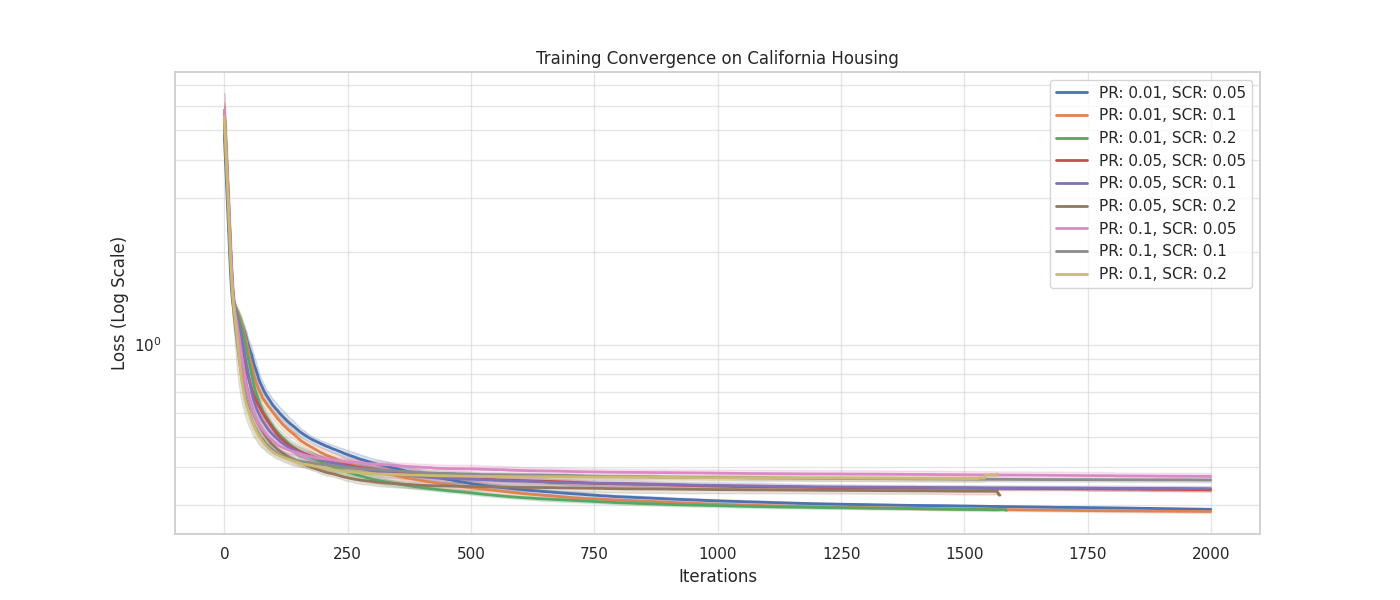
\includegraphics[width=0.9\textwidth]{figures/results/small_net_random_sampling_grid_search/small_net_random_sampling_grid_search_convergence.png}
    \caption{Training convergence for Small Net using various Random Sampling configurations (Log Scale).}
    \label{fig:small_net_random_convergence}
\end{figure}


The configurations with a lower perturbation ratio ($1\%$, depicted in blue and green hues) exhibit the most stable and deepest descent. As the perturbation ratio increases to $5\%$ and $10\%$, the algorithm struggles to refine the solution, likely due to "jumping" over narrow local minima.

\newpage

The stability of these stochastic updates is further examined in the final loss distribution shown in Figure \ref{fig:small_net_random_final_loss}.

\begin{figure}[htbp]
    \centering
    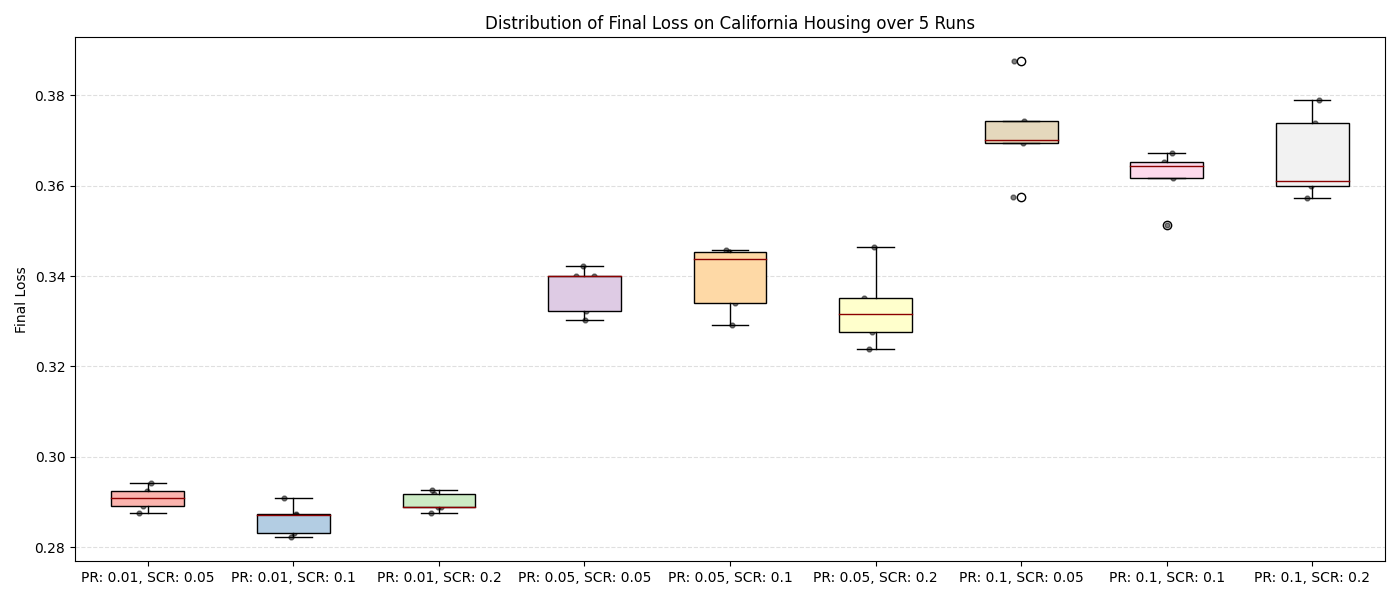
\includegraphics[width=0.85\textwidth]{figures/results/small_net_random_sampling_grid_search/small_net_random_sampling_grid_search_final_loss.png}
    \caption{Distribution of Final Loss over 5 runs across the grid search space.}
    \label{fig:small_net_random_final_loss}
\end{figure}


The best performing configuration is \textbf{Perturbation Ratio: 0.01} with a \textbf{Search Ratio: 0.1}, which achieves the lowest average loss with remarkably low variance. Interestingly, increasing coverage (Search Ratio) from $0.1$ to $0.2$ does not significantly improve the final loss for the $0.01$ perturbation case, but it substantially increases the computational time.

\newpage

The regression metrics across the grid are summarized in Figure \ref{fig:small_net_random_metrics_dist}.

\begin{figure}[htbp]
    \centering
    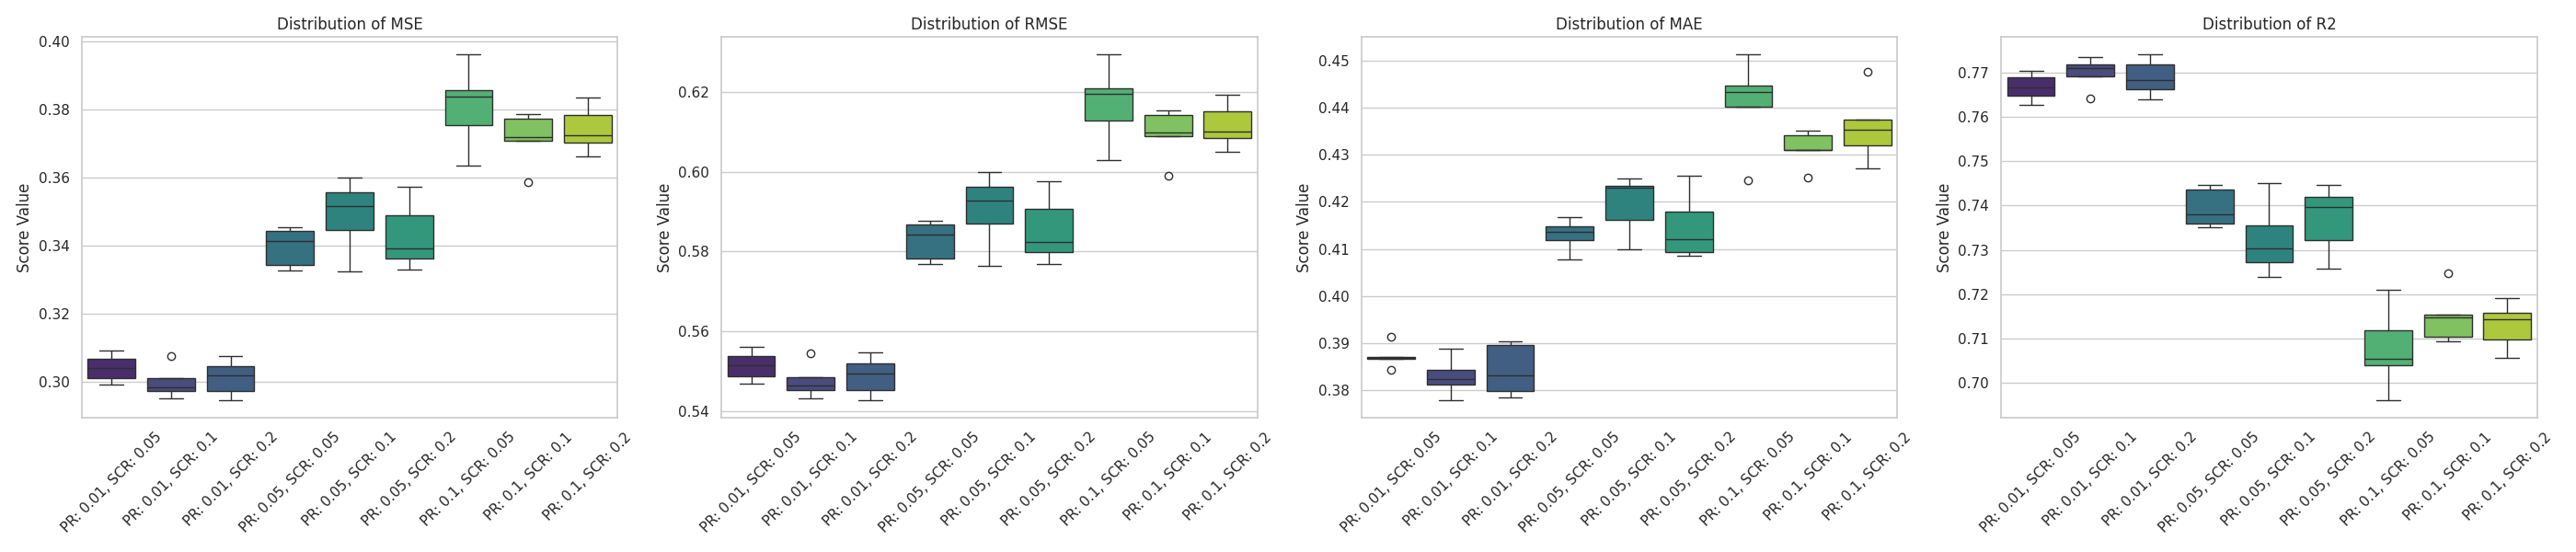
\includegraphics[width=1\textwidth]{figures/results/small_net_random_sampling_grid_search/small_net_random_sampling_grid_search_metrics_distribution.png}
    \caption{Distribution of MSE, RMSE, MAE, and $R^2$ for the Random Sampling Grid Search.}
    \label{fig:small_net_random_metrics_dist}
\end{figure}

The $R^2$ scores confirm that smaller perturbations are vastly superior for this task, with configurations at $1\%$ perturbation reaching $R^2$ values near $0.77$. This suggests that for a network of this size, high-precision, small-scale stochastic adjustments are more effective than larger, more aggressive updates.

\subsubsection{Summary Statistics}

Tables below provide the numerical breakdown of the average performance for each tested configuration.

\begin{table}[h]
\centering
\scriptsize
\begin{tabular}{|l|c|c|c|c|c|}
\hline
\textbf{Pert. / Search} & \textbf{0.01 / 0.05} & \textbf{0.01 / 0.1} & \textbf{0.01 / 0.2} & \textbf{0.05 / 0.05} & \textbf{0.05 / 0.1} \\ \hline
Avg Final Loss & 0.2909 & 0.2862 & 0.2900 & 0.3369 & 0.3396 \\ \hline
Avg Time (s)   & 325.44 & 562.40 & 855.63 & 278.16 & 535.81 \\ \hline
Avg MSE        & 0.3040 & 0.2998 & 0.3012 & 0.3396 & 0.3488 \\ \hline
Avg RMSE       & 0.5514 & 0.5476 & 0.5488 & 0.5827 & 0.5905 \\ \hline
Avg MAE        & 0.3872 & 0.3829 & 0.3843 & 0.4130 & 0.4195 \\ \hline
Avg $R^2$      & 0.7668 & 0.7700 & 0.7689 & 0.7395 & 0.7324 \\ \hline
\end{tabular}
\caption{Average statistical metrics for Small Net Random Sampling (Part 1).}
\label{tab:small_net_random_part1}
\end{table}

\newpage

\begin{table}[h]
\centering
\scriptsize
\begin{tabular}{|l|c|c|c|c|}
\hline
\textbf{Pert. / Search} & \textbf{0.05 / 0.2} & \textbf{0.1 / 0.05} & \textbf{0.1 / 0.1} & \textbf{0.1 / 0.2} \\ \hline
Avg Final Loss & 0.3329 & 0.3718 & 0.3620 & 0.3662 \\ \hline
Avg Time (s)   & 823.20 & 270.92 & 524.14 & 805.04 \\ \hline
Avg MSE        & 0.3429 & 0.3810 & 0.3715 & 0.3741 \\ \hline
Avg RMSE       & 0.5855 & 0.6172 & 0.6095 & 0.6116 \\ \hline
Avg MAE        & 0.4148 & 0.4408 & 0.4313 & 0.4359 \\ \hline
Avg $R^2$      & 0.7369 & 0.7077 & 0.7150 & 0.7130 \\ \hline
\end{tabular}
\caption{Average statistical metrics for Small Net Random Sampling (Part 2).}
\label{tab:small_net_random_part2}
\end{table}

\subsection{Medium Net Results}

For the Medium Net architecture, the grid search was conducted using the same parameter combinations to assess how increased network complexity influences sampling dynamics:
\begin{itemize}
    \item \textbf{Perturbation Ratios:} $[0.01, 0.05, 0.1]$ ($1\%, 5\%, 10\%$).
    \item \textbf{Search Coverage Ratios:} $[0.05, 0.1, 0.2]$ ($5\%, 10\%, 20\%$).
    \item \textbf{Iterations:} 2000.
    \item \textbf{Runs:} 5 for each unique pair.
\end{itemize}

\newpage

\subsubsection{Visual Analysis of Convergence and Loss Distribution}

The training trajectories for the nine configurations on the Medium Net are illustrated in Figure \ref{fig:medium_net_random_convergence}.

\begin{figure}[htbp]
    \centering
    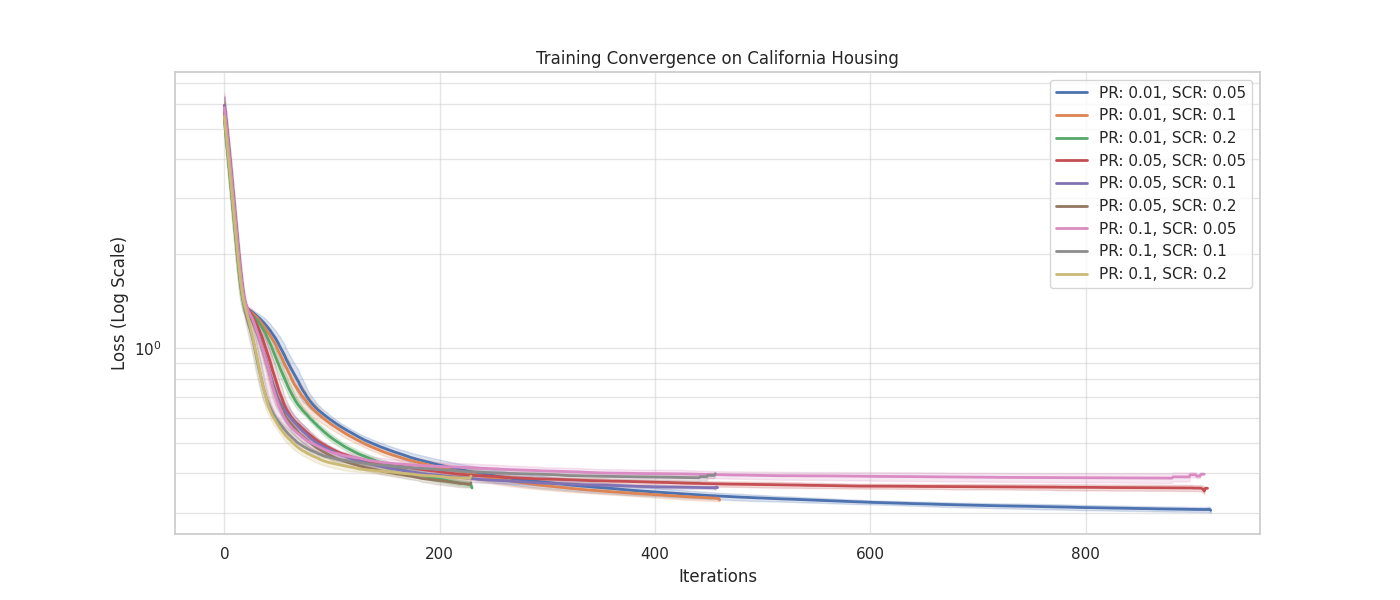
\includegraphics[width=0.9\textwidth]{figures/results/medium_net_random_sampling_grid_search/medium_net_random_sampling_grid_search_convergence.png}
    \caption{Training convergence for Medium Net using various Random Sampling configurations (Log Scale).}
    \label{fig:medium_net_random_convergence}
\end{figure}

In this architecture, sensitivity to the \textit{perturbation ratio} remains the dominant factor. It is observed that the configuration with $1\%$ perturbation and $5\%$ coverage (Pert. Ratio: 0.01, Search Ratio: 0.05) produces the most rapid and deepest descent. Compared to the Small Net, the increased number of parameters seems to make a very narrow local search (low Search Ratio) more effective, indicating that in higher-dimensional spaces, over-exploration through too many random directions can be less efficient than precision in individual steps.

\newpage

The stability of these stochastic updates is further examined in the final loss distribution shown in Figure \ref{fig:medium_net_random_final_loss}.

\begin{figure}[htbp]
    \centering
    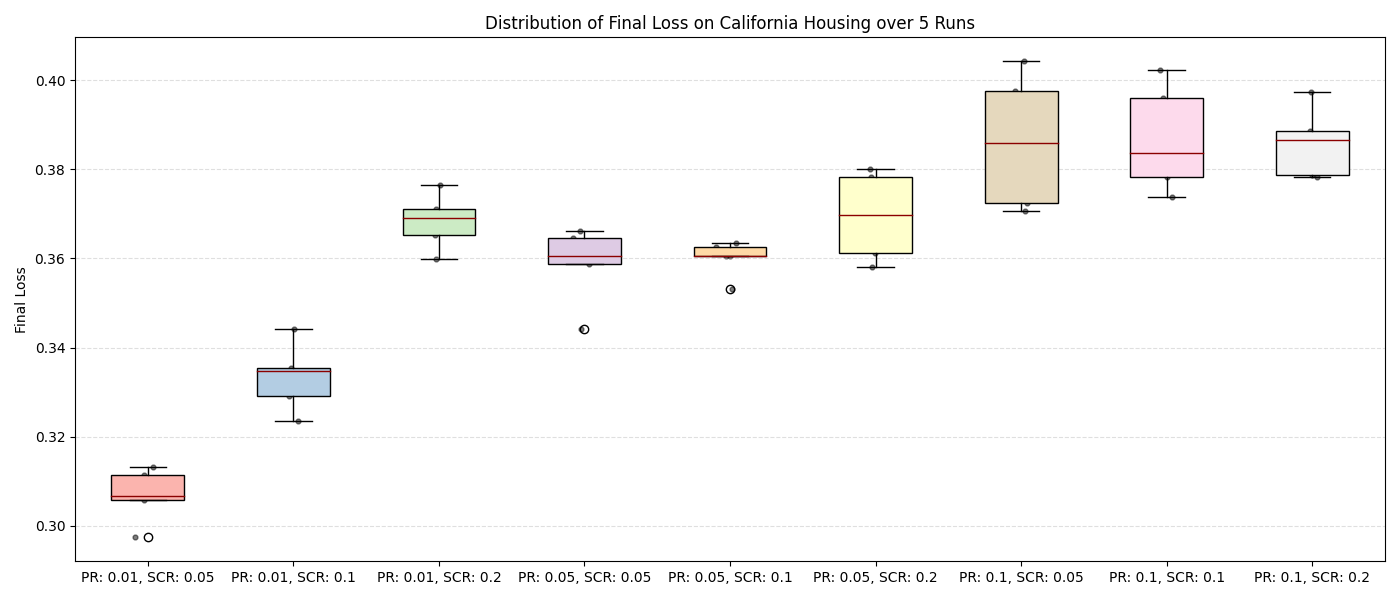
\includegraphics[width=0.85\textwidth]{figures/results/medium_net_random_sampling_grid_search/medium_net_random_sampling_grid_search_final_loss.png}
    \caption{Distribution of Final Loss over 5 runs across the grid search space for Medium Net.}
    \label{fig:medium_net_random_final_loss}
\end{figure}

The \textbf{Perturbation Ratio: 0.01} with \textbf{Search Ratio: 0.05} configuration is confirmed as the best performer, achieving the lowest average loss ($0.3068$) with extremely low variance ($0.000030$). Interestingly, for this network, increasing the coverage (Search Ratio) to $0.1$ or $0.2$ actually degrades the final loss, suggesting a risk of over-exploration that leads the algorithm away from the most promising local minima.

\newpage

The regression metrics for the Medium Net are summarized in Figure \ref{fig:medium_net_random_metrics_dist}.

\begin{figure}[htbp]
    \centering
    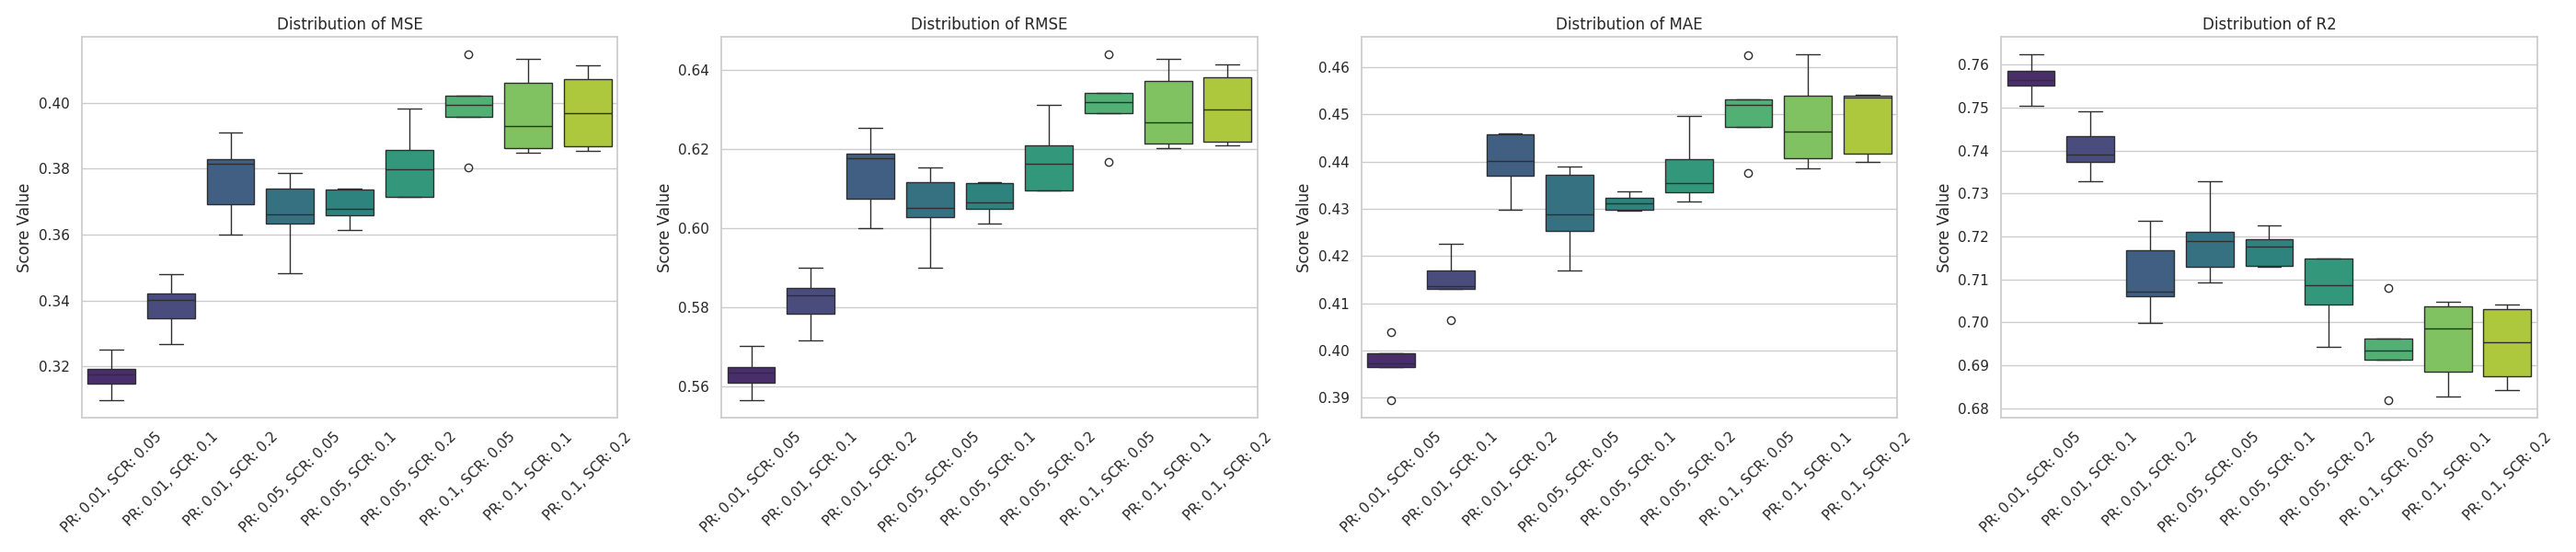
\includegraphics[width=1\textwidth]{figures/results/medium_net_random_sampling_grid_search/medium_net_random_sampling_grid_search_metrics_distribution.png}
    \caption{Distribution of MSE, RMSE, MAE, and $R^2$ for the Medium Net Random Sampling Grid Search.}
    \label{fig:medium_net_random_metrics_dist}
\end{figure}

The $R^2$ scores highlight that predictive performance decreases linearly as the perturbation increases. The optimal configuration reaches an average $R^2$ of approximately $0.7566$, demonstrating that even with a deeper network, random sampling with small increments is capable of effectively modeling the California Housing dataset.

\subsubsection{Summary Statistics}

The tables below provide the numerical breakdown of the average performance for each tested configuration on the Medium Net architecture.

\begin{table}[h]
\centering
\scriptsize
\begin{tabular}{|l|c|c|c|c|c|}
\hline
\textbf{Pert. / Search} & \textbf{0.01 / 0.05} & \textbf{0.01 / 0.1} & \textbf{0.01 / 0.2} & \textbf{0.05 / 0.05} & \textbf{0.05 / 0.1} \\ \hline
Avg Final Loss & 0.3068 & 0.3334 & 0.3684 & 0.3588 & 0.3601 \\ \hline
Avg Time (s)   & 802.43 & 790.59 & 781.27 & 788.71 & 783.09 \\ \hline
Avg MSE        & 0.3173 & 0.3384 & 0.3770 & 0.3662 & 0.3686 \\ \hline
Avg RMSE       & 0.5632 & 0.5817 & 0.6139 & 0.6051 & 0.6071 \\ \hline
Avg MAE        & 0.3973 & 0.4145 & 0.4397 & 0.4295 & 0.4313 \\ \hline
Avg $R^2$      & 0.7566 & 0.7404 & 0.7108 & 0.7191 & 0.7172 \\ \hline
\end{tabular}
\caption{Average statistical metrics for Medium Net Random Sampling (Part 1).}
\label{tab:medium_net_random_part1}
\end{table}

\newpage

\begin{table}[h]
\centering
\scriptsize
\begin{tabular}{|l|c|c|c|c|}
\hline
\textbf{Pert. / Search} & \textbf{0.05 / 0.2} & \textbf{0.1 / 0.05} & \textbf{0.1 / 0.1} & \textbf{0.1 / 0.2} \\ \hline
Avg Final Loss & 0.3695 & 0.3862 & 0.3868 & 0.3859 \\ \hline
Avg Time (s)   & 777.98 & 774.91 & 775.43 & 779.09 \\ \hline
Avg MSE        & 0.3814 & 0.3985 & 0.3967 & 0.3976 \\ \hline
Avg RMSE       & 0.6175 & 0.6312 & 0.6297 & 0.6305 \\ \hline
Avg MAE        & 0.4382 & 0.4505 & 0.4485 & 0.4486 \\ \hline
Avg $R^2$      & 0.7074 & 0.6942 & 0.6957 & 0.6949 \\ \hline
\end{tabular}
\caption{Average statistical metrics for Medium Net Random Sampling (Part 2).}
\label{tab:medium_net_random_part2}
\end{table}


\subsection{Big Net Results}

For the Big Net architecture, the grid search explores how stochastic optimization scales with a significantly larger parameter space. The test conditions remain consistent with the previous architectures:
\begin{itemize}
    \item \textbf{Perturbation Ratios:} $[0.01, 0.05, 0.1]$ ($1\%, 5\%, 10\%$).
    \item \textbf{Search Coverage Ratios:} $[0.05, 0.1, 0.2]$ ($5\%, 10\%, 20\%$).
    \item \textbf{Iterations:} 2000.
    \item \textbf{Runs:} 5 for each unique pair.
\end{itemize}

\newpage

\subsubsection{Visual Analysis of Convergence and Loss Distribution}

The training trajectories for the Big Net are presented in Figure \ref{fig:big_net_random_convergence}. 

\begin{figure}[htbp]
    \centering
    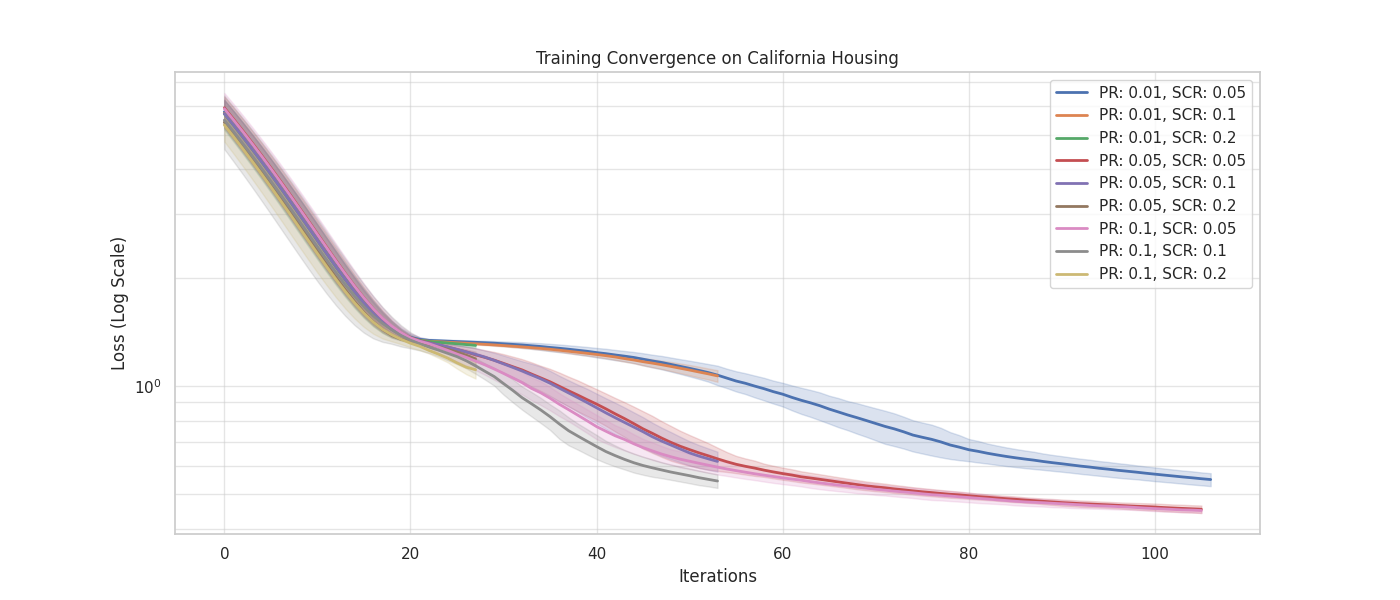
\includegraphics[width=0.9\textwidth]{figures/results/big_net_random_sampling_grid_search/big_net_random_sampling_grid_search_convergence.png}
    \caption{Training convergence for Big Net using various Random Sampling configurations (Log Scale).}
    \label{fig:big_net_random_convergence}
\end{figure}

A significant shift in behavior is observed compared to the smaller networks. While in the Small Net a low perturbation was universally better, the Big Net shows that a higher \textit{Perturbation Ratio} ($0.05$ or $0.1$), when paired with a very low \textit{Search Coverage Ratio} ($0.05$), results in the most effective optimization. This suggests that in high-dimensional spaces, making more substantial updates to a smaller number of candidate neighbors is more effective than fine-grained updates across a wide search breadth.

\newpage

The distribution of final loss values is shown in Figure \ref{fig:big_net_random_final_loss}, highlighting a clear "curse of dimensionality" effect.

\begin{figure}[htbp]
    \centering
    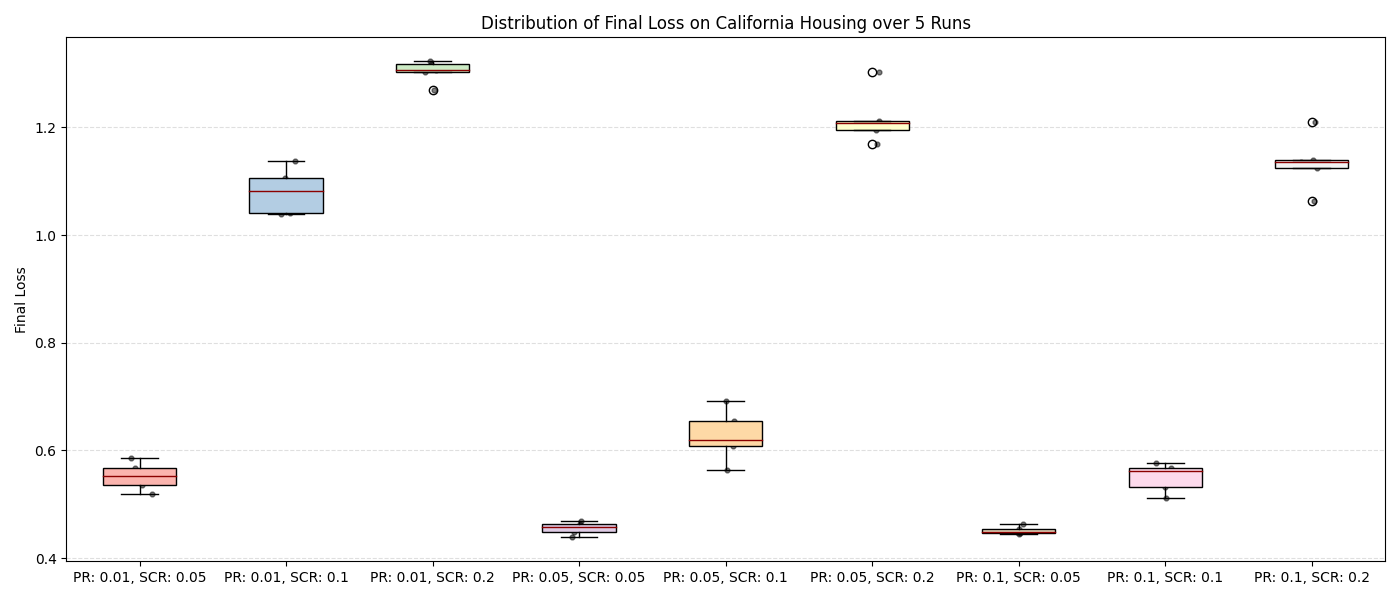
\includegraphics[width=0.85\textwidth]{figures/results/big_net_random_sampling_grid_search/big_net_random_sampling_grid_search_final_loss.png}
    \caption{Distribution of Final Loss over 5 runs across the grid search space for Big Net.}
    \label{fig:big_net_random_final_loss}
\end{figure}

The best-performing configurations are \textbf{Perturbation Ratio: 0.1 / Search Ratio: 0.05} (Avg Loss: $0.4518$) and \textbf{Perturbation Ratio: 0.05 / Search Ratio: 0.05} (Avg Loss: $0.4554$). Conversely, any configuration with a high Search Ratio ($0.2$) performs poorly, with losses exceeding $1.1$, indicating that searching too many random directions in such a large space leads to a lack of refinement.

\newpage

The regression metrics for the Big Net are visualized in Figure \ref{fig:big_net_random_metrics_dist}.

\begin{figure}[htbp]
    \centering
    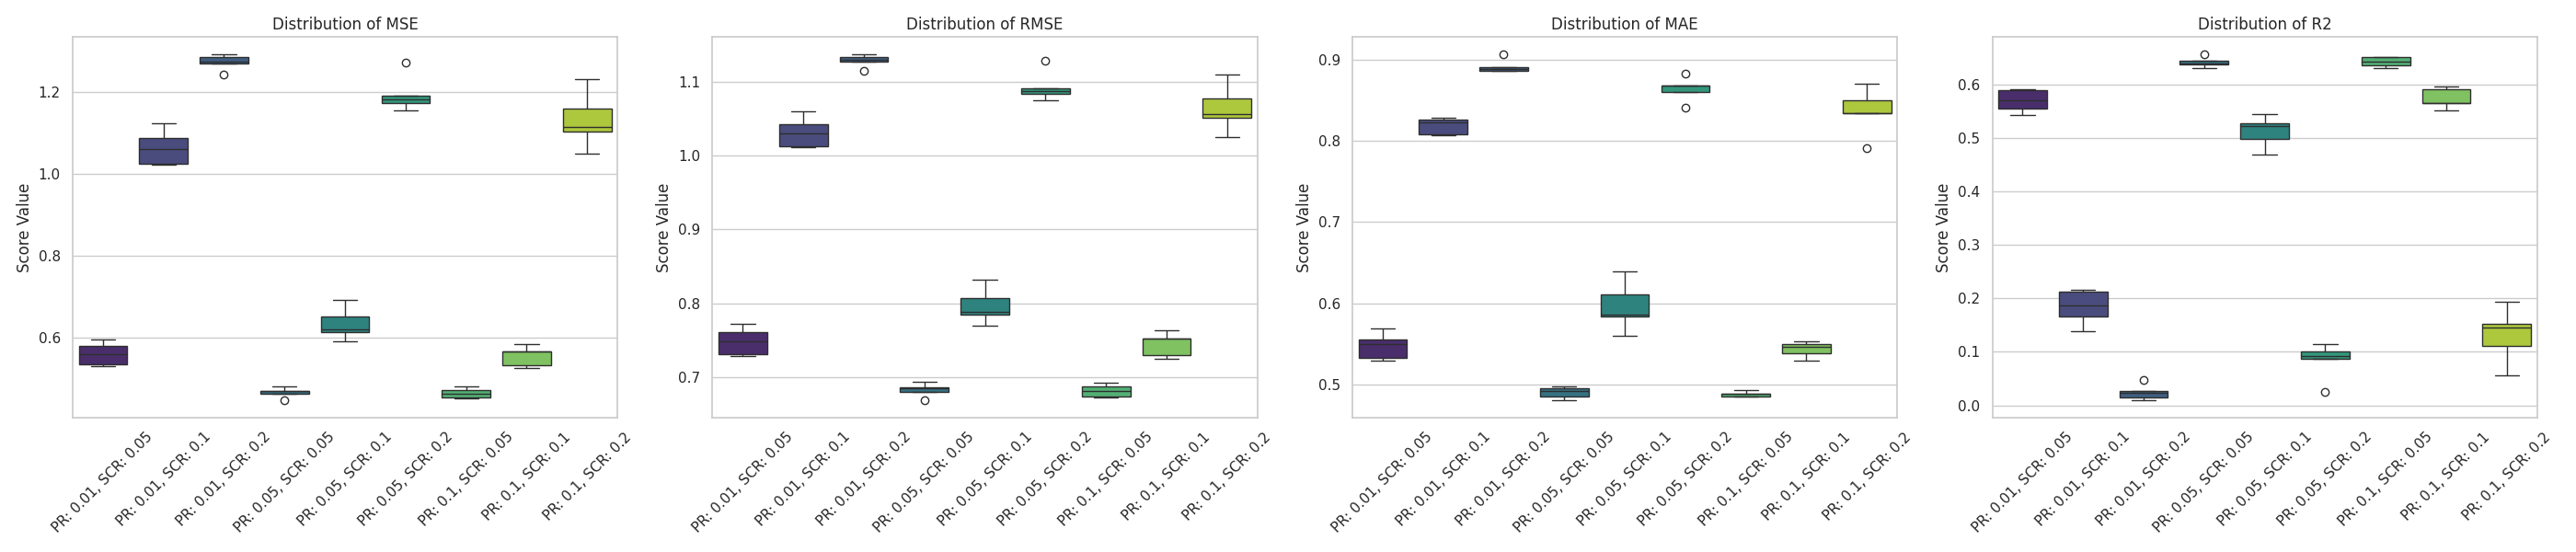
\includegraphics[width=1\textwidth]{figures/results/big_net_random_sampling_grid_search/big_net_random_sampling_grid_search_metrics_distribution.png}
    \caption{Distribution of MSE, RMSE, MAE, and $R^2$ for the Big Net Random Sampling Grid Search.}
    \label{fig:big_net_random_metrics_dist}
\end{figure}

The $R^2$ scores confirm that the predictive power of the model is highly sensitive to the search ratio in large networks. The optimal configurations reach an $R^2$ of approximately $0.6428$. However, when the Search Ratio increases to $0.2$, the $R^2$ drops dramatically toward zero ($0.02$ to $0.13$), showing that the algorithm fails to find a meaningful mapping when the search is too broad and stochastic.

\subsubsection{Summary Statistics}

The tables below summarize the average statistical performance for all tested configurations on the Big Net.

\begin{table}[h]
\centering
\scriptsize
\begin{tabular}{|l|c|c|c|c|c|}
\hline
\textbf{Pert. / Search} & \textbf{0.01 / 0.05} & \textbf{0.01 / 0.1} & \textbf{0.01 / 0.2} & \textbf{0.05 / 0.05} & \textbf{0.05 / 0.1} \\ \hline
Avg Final Loss & 0.5523 & 1.0809 & 1.3036 & 0.4554 & 0.6274 \\ \hline
Avg Time (s)   & 733.17 & 726.02 & 739.29 & 727.94 & 729.05 \\ \hline
Avg MSE        & 0.5609 & 1.0637 & 1.2724 & 0.4671 & 0.6351 \\ \hline
Avg RMSE       & 0.7488 & 1.0312 & 1.1280 & 0.6834 & 0.7967 \\ \hline
Avg MAE        & 0.5471 & 0.8186 & 0.8918 & 0.4898 & 0.5959 \\ \hline
Avg $R^2$      & 0.5696 & 0.1839 & 0.0238 & 0.6416 & 0.5127 \\ \hline
\end{tabular}
\caption{Average statistical metrics for Big Net Random Sampling (Part 1).}
\label{tab:big_net_random_part1}
\end{table}

\newpage

\begin{table}[h]
\centering
\scriptsize
\begin{tabular}{|l|c|c|c|c|}
\hline
\textbf{Pert. / Search} & \textbf{0.05 / 0.2} & \textbf{0.1 / 0.05} & \textbf{0.1 / 0.1} & \textbf{0.1 / 0.2} \\ \hline
Avg Final Loss & 1.2176 & 0.4518 & 0.5501 & 1.1347 \\ \hline
Avg Time (s)   & 739.12 & 727.02 & 730.05 & 735.02 \\ \hline
Avg MSE        & 1.1942 & 0.4656 & 0.5557 & 1.1316 \\ \hline
Avg RMSE       & 1.0927 & 0.6823 & 0.7453 & 1.0634 \\ \hline
Avg MAE        & 0.8643 & 0.4882 & 0.5433 & 0.8360 \\ \hline
Avg $R^2$      & 0.0837 & 0.6428 & 0.5737 & 0.1318 \\ \hline
\end{tabular}
\caption{Average statistical metrics for Big Net Random Sampling (Part 2).}
\label{tab:big_net_random_part2}
\end{table}


\subsection{Conclusion on Random Neighbors Generation Study}

The grid search analysis conducted across Small, Medium, and Big Net architectures provides several key insights into the behavior of stochastic training within a discrete state-space search.

\begin{itemize}
    \item \textbf{Architecture-Dependent Sensitivity:} The study demonstrates that the optimal hyperparameter configuration is strictly linked to the network's dimensionality. For the \textbf{Small Net}, a fine-grained approach (1\% perturbation with 10\% coverage) yielded the best results. However, as the parameter space expanded in the \textbf{Big Net}, the algorithm required more aggressive updates (5-10\% perturbation) but a much narrower search breadth (5\% coverage) to avoid the "noise" of excessive random exploration.
    
    \item \textbf{The Optimal Hyperparameter Window:} Despite architectural variances, the most effective configurations consistently fell within a specific range: \textbf{Perturbation Ratios} between $[0.01, 0.1]$ and \textbf{Search Coverage Ratios} between $[0.05, 0.1]$. Deviating outside these bounds — particularly by increasing search coverage to 20\% — consistently resulted in diminishing returns or performance degradation due to over-exploration.
    
    \item \textbf{Stochastic vs. Deterministic Search:} Most significantly, the random sampling approach consistently outperformed the kernel-based methods tested in previous sections. While kernels provide a structured update, random sampling allows the $A^*$ algorithm to explore a more diverse set of directions in the weight landscape. This stochasticity appears to be a \textbf{primary driver for performance}, enabling the model to achieve higher $R^2$ scores and lower MSE values across all tested architectures.
    
    \item \textbf{Computational Efficiency:} Random sampling proved to be computationally robust. Even with lower search coverage, the ability to find high-quality descent directions allowed for faster convergence compared to static high-resolution quantization methods, making it a highly scalable alternative for complex neural network training.
\end{itemize}

In conclusion, \textbf{Random Neighbors Generation} transforms the training process into a more effective stochastic optimization task. By balancing the intensity of updates with a controlled search breadth, this method provides a superior ability to navigate the complex loss surfaces of deep learning models compared to rigid, kernel-driven architectures.


%%%%%%%%%%%%%%%%%% NEIGHBORS GENERATION STRATEGIES %%%%%%%%%%%%%%%%%%%%%%%%%%%%%%%%
\section{Neighbors Generation Strategies Comparison}
\label{sec:strategies_comparison}

This section evaluates and compares the three proposed neighbor generation strategies—\textit{Single Kernel}, \textit{Layer-wise Kernels}, and \textit{Random Neighbors Generation}—using the optimal hyperparameters identified in the previous tuning phases. To isolate the intrinsic performance of each generation logic, the Beam Search optimization is omitted in these tests.

The goal is to determine which strategy provides the most effective exploration of the weight space and achieves the lowest convergence error on the California Housing benchmark.

\subsection{Small Net Results}

The Small Net architecture was tested using the following optimized configurations:
\begin{itemize}
    \item \textbf{Single Kernel:} Weight kernel $[2,2]$, Bias kernel $[2]$, Stride 2.
    \item \textbf{Layer-wise Kernels:} 
        \begin{itemize}
            \item Weight kernels: $[[2,2], [2,2], [1,2]]$
            \item Bias kernels: $[[2], [2], [1]]$
            \item Weight strides: $[[2,2], [2,2], [2,1]]$
            \item Bias strides: $[[2], [2], [1]]$
        \end{itemize}
    \item \textbf{Random Sampling:} Perturbation ratio 0.01, Search coverage ratio 0.1.
\end{itemize}

\newpage

\subsubsection{Visual Analysis of Training and Stability}

The training convergence comparison is illustrated in Figure \ref{fig:small_net_comp_convergence}. While all strategies exhibit a similar initial descent, a significant gap emerges after the first 250 iterations.

\begin{figure}[htbp]
    \centering
    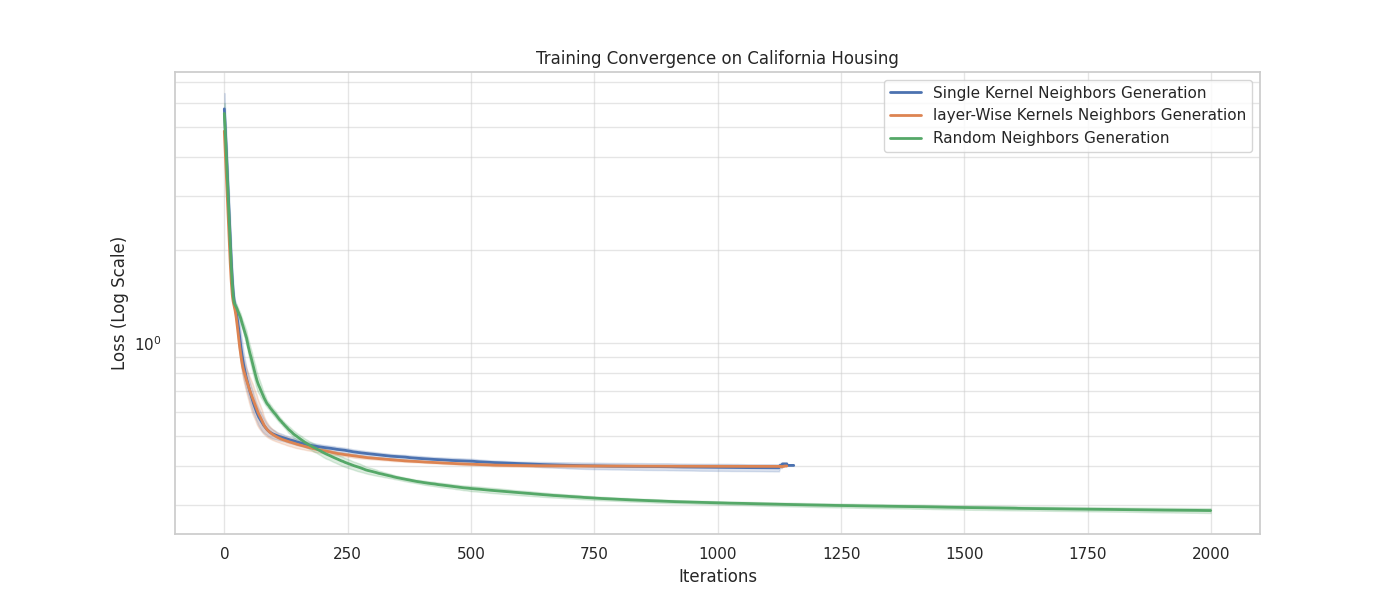
\includegraphics[width=0.9\textwidth]{figures/results/small_net_neighbors_generation_strategies_comparison_no_BS/small_net_neighbors_generation_strategies_comparison_no_BS_convergence.png}
    \caption{Training convergence comparison between Single Kernel, Layer-wise, and Random strategies (Log Scale).}
    \label{fig:small_net_comp_convergence}
\end{figure}

The \textit{Random Neighbors Generation} strategy (green line) shows a markedly superior convergence profile, continuing to reduce the loss long after the kernel-based methods have reached a plateau. This suggests that stochastic sampling allows the $A^*$ algorithm to navigate the high-dimensional loss surface more flexibly than the fixed structural updates of the kernel methods.

\newpage
The distribution of the final loss values across 5 independent runs is shown in Figure \ref{fig:small_net_comp_final_loss}.

\begin{figure}[htbp]
    \centering
    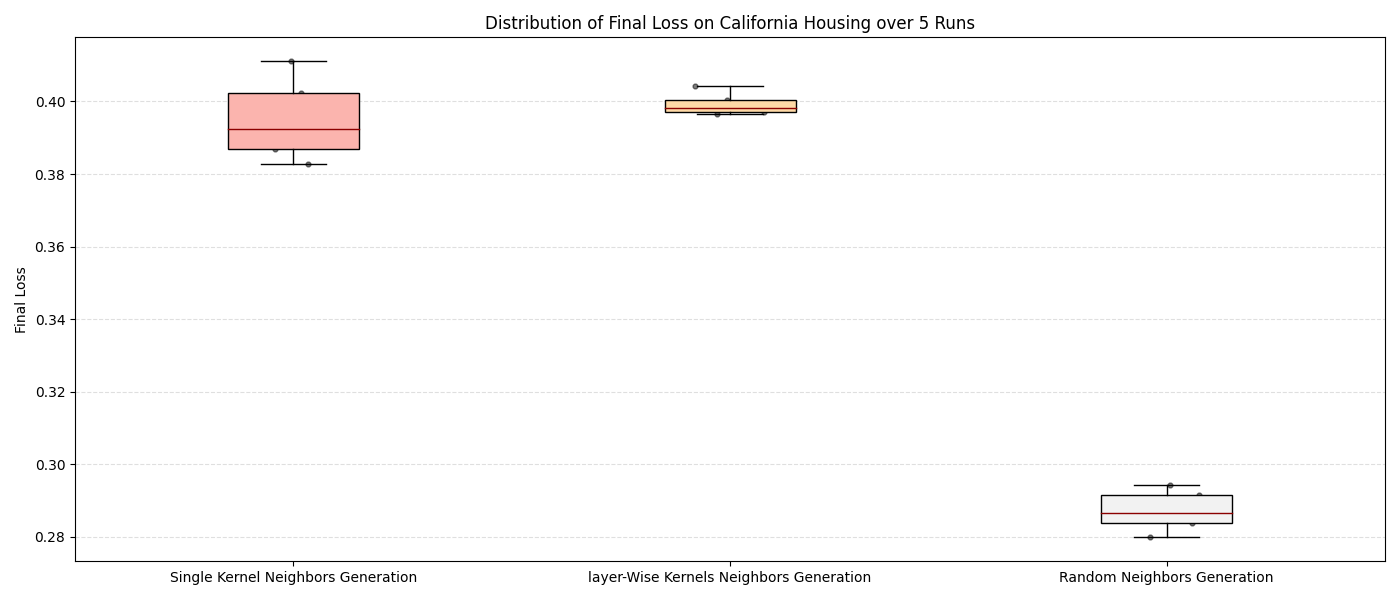
\includegraphics[width=0.85\textwidth]{figures/results/small_net_neighbors_generation_strategies_comparison_no_BS/small_net_neighbors_generation_strategies_comparison_no_BS_final_loss.png}
    \caption{Distribution of Final Loss for the three generation strategies on Small Net.}
    \label{fig:small_net_comp_final_loss}
\end{figure}

The boxplot confirms that the Random strategy is not only more effective but also highly stable, maintaining a lower median loss (~0.286) compared to the Single Kernel (~0.392) and Layer-wise (~0.398) approaches.

\newpage

The regression metrics for the Small Net are visualized in Figure \ref{fig:small_net_comp_metrics_dist}.

\begin{figure}[htbp]
    \centering
    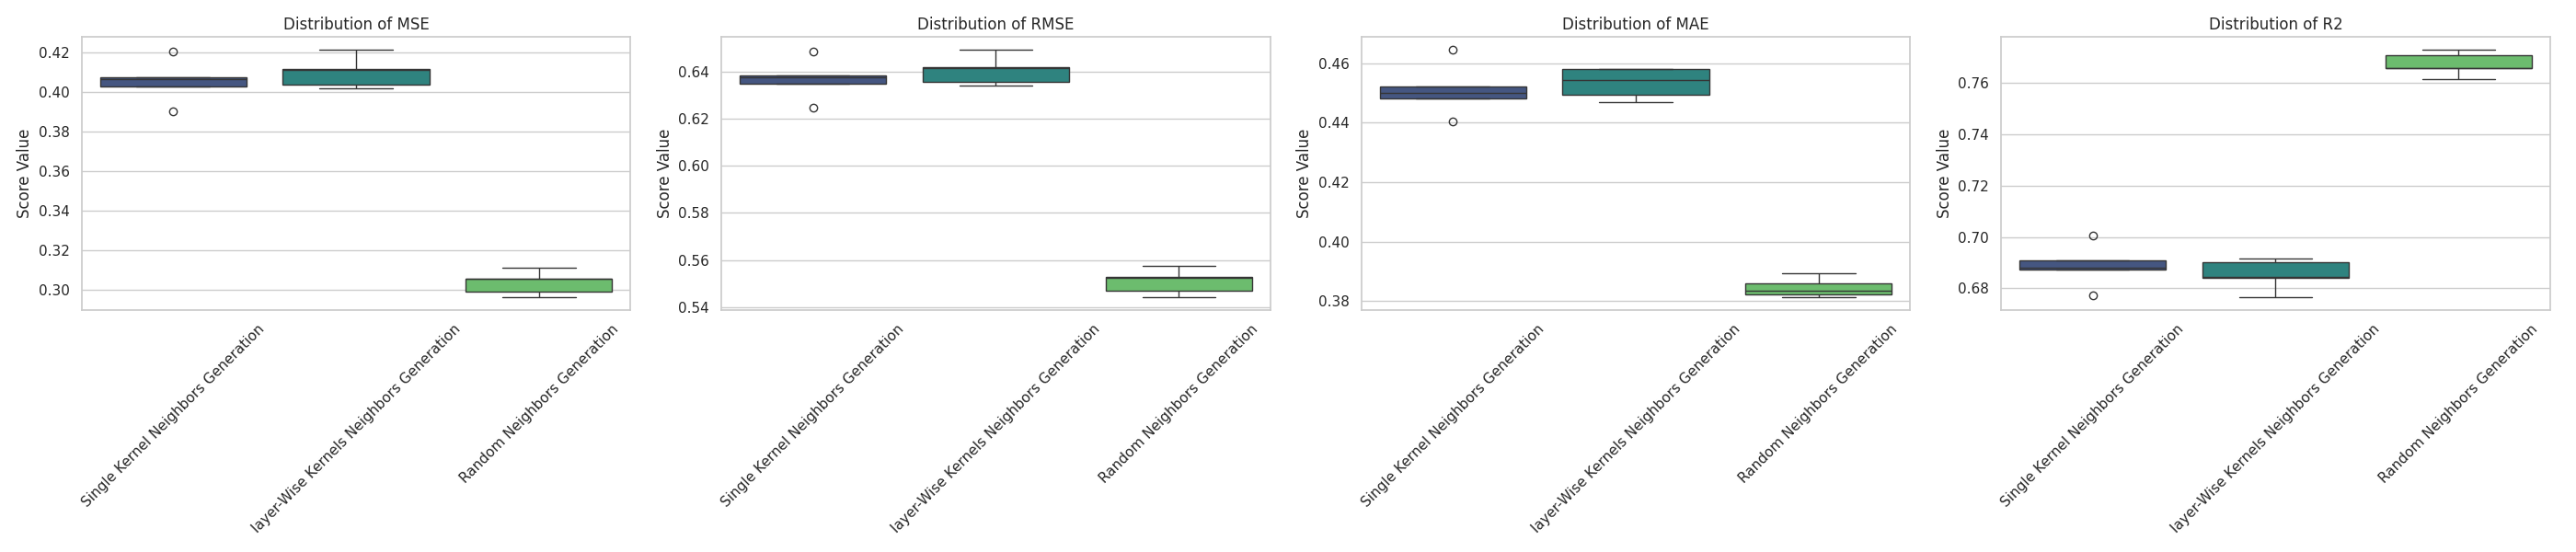
\includegraphics[width=1\textwidth]{figures/results/small_net_neighbors_generation_strategies_comparison_no_BS/small_net_neighbors_generation_strategies_comparison_no_BS_metrics_distribution.png}
    \caption{Regression metrics distribution (MSE, RMSE, MAE, $R^2$) across generation strategies.}
    \label{fig:small_net_comp_metrics_dist}
\end{figure}

The $R^2$ scores further validate the superiority of the Random approach, which achieves values centered around 0.77, whereas both kernel strategies cluster significantly lower, near 0.69.

\subsubsection{Summary Statistics}

The numerical performance summary in Table \ref{tab:small_net_comp_results_fixed} highlights the clear advantage of stochastic sampling for this architecture.

\begin{table}[h]
\centering
\scriptsize
\begin{tabular}{|l|c|c|c|}
\hline
\textbf{Metric (Avg)} & \textbf{Random (0.01 / 0.1)} & \textbf{Single Kernel} & \textbf{Layer-wise Kernels} \\ \hline
Avg Final Loss        & 0.2872                       & 0.3951                 & 0.3993                      \\ \hline
Avg Time (s)          & 535.60                       & 777.80                 & 753.39                      \\ \hline
Avg MSE               & 0.3035                       & 0.4055                 & 0.4101                      \\ \hline
Avg RMSE              & 0.5508                       & 0.6368                 & 0.6404                      \\ \hline
Avg MAE               & 0.3844                       & 0.4511                 & 0.4534                      \\ \hline
Avg $R^2$             & 0.7672                       & 0.6889                 & 0.6853                      \\ \hline
\end{tabular}
\caption{Average statistical comparison of generation strategies for Small Net.}
\label{tab:small_net_comp_results_fixed}
\end{table}


\subsection{Medium Net Results}

The Medium Net architecture was evaluated using the optimal settings derived from the previous grid search. The configurations compared are:
\begin{itemize}
    \item \textbf{Single Kernel:} Weight kernel $[4,4]$, Bias kernel $[4]$, Stride 4.
    \item \textbf{Layer-wise Kernels:} 
        \begin{itemize}
            \item Weight kernels: $[[4,4], [4,4], [4,4], [1,4]]$
            \item Bias kernels: $[[4], [4], [4], [1]]$
            \item Weight strides: $[[4,4], [4,4], [4,4], [4,1]]$
            \item Bias strides: $[[4], [4], [4], [1]]$
        \end{itemize}
    \item \textbf{Random Sampling:} Perturbation ratio 0.01, Search coverage ratio 0.05.
\end{itemize}

\subsubsection{Visual Analysis of Training and Stability}

The convergence dynamics for the Medium Net, shown in Figure \ref{fig:medium_net_comp_convergence}, reveal that the gap between stochastic and deterministic strategies widens as network depth increases.

\begin{figure}[htbp]
    \centering
    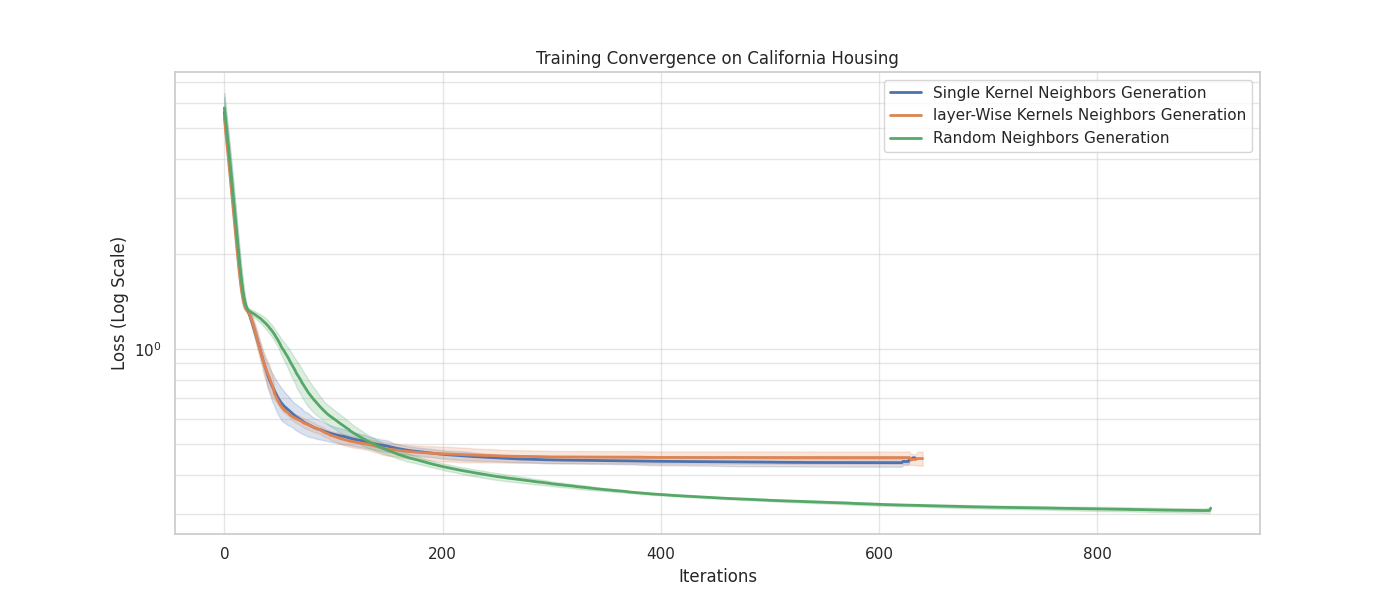
\includegraphics[width=0.9\textwidth]{figures/results/medium_net_neighbors_generation_strategies_comparison_no_BS/medium_net_neighbors_generation_strategies_comparison_no_BS_convergence.png}
    \caption{Training convergence comparison for Medium Net (Log Scale).}
    \label{fig:medium_net_comp_convergence}
\end{figure}

The \textit{Random Neighbors Generation} (green line) continues to refine the loss effectively, whereas both the \textit{Single Kernel} and \textit{Layer-wise} methods reach a performance plateau relatively early, around iteration 400. This confirms that for larger architectures, the rigid geometric updates of kernels struggle to find effective descent directions in a more complex parameter space.

The stability of these results is analyzed through the distribution of the final loss in Figure \ref{fig:medium_net_comp_final_loss}.

\newpage

\begin{figure}[htbp]
    \centering
    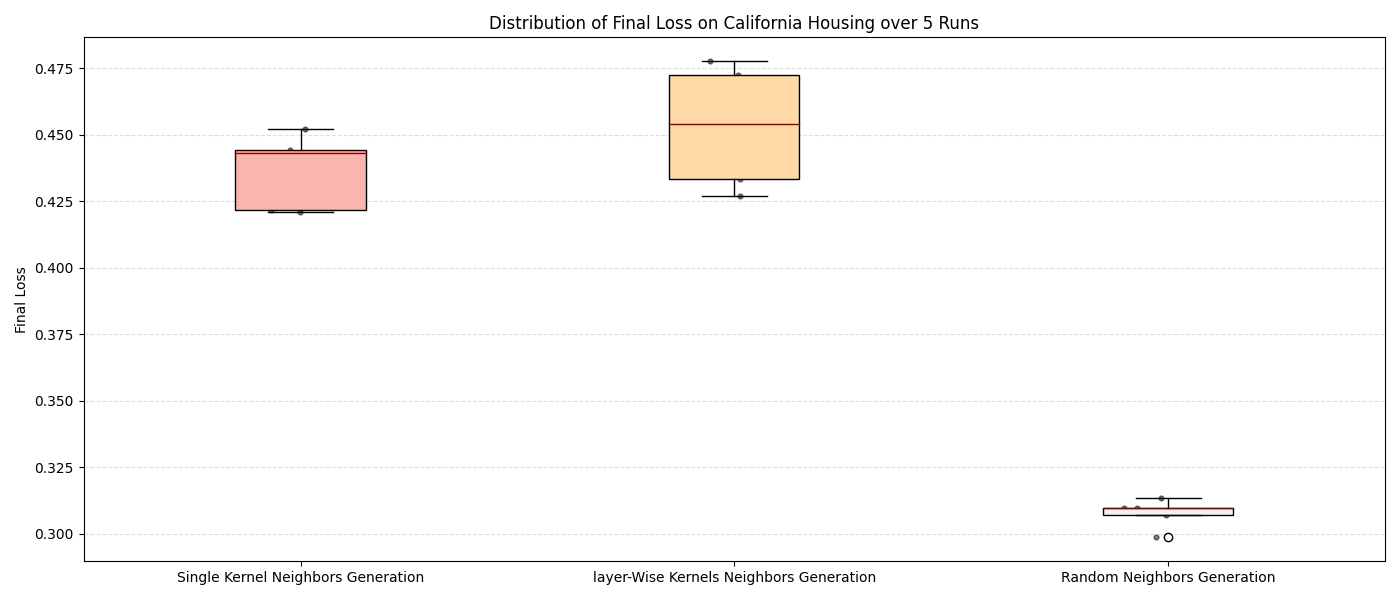
\includegraphics[width=0.85\textwidth]{figures/results/medium_net_neighbors_generation_strategies_comparison_no_BS/medium_net_neighbors_generation_strategies_comparison_no_BS_final_loss.png}
    \caption{Distribution of Final Loss for Medium Net generation strategies.}
    \label{fig:medium_net_comp_final_loss}
\end{figure}

The Random approach maintains a significantly lower and more consistent final loss ($0.3076$). In contrast, the \textit{Layer-wise} method exhibits the highest average loss ($0.4529$), suggesting that the additional complexity of per-layer kernels does not translate to better optimization in this specific architecture.

\newpage

The distribution of regression metrics for the Medium Net is summarized in Figure \ref{fig:medium_net_comp_metrics_dist}.

\begin{figure}[htbp]
    \centering
    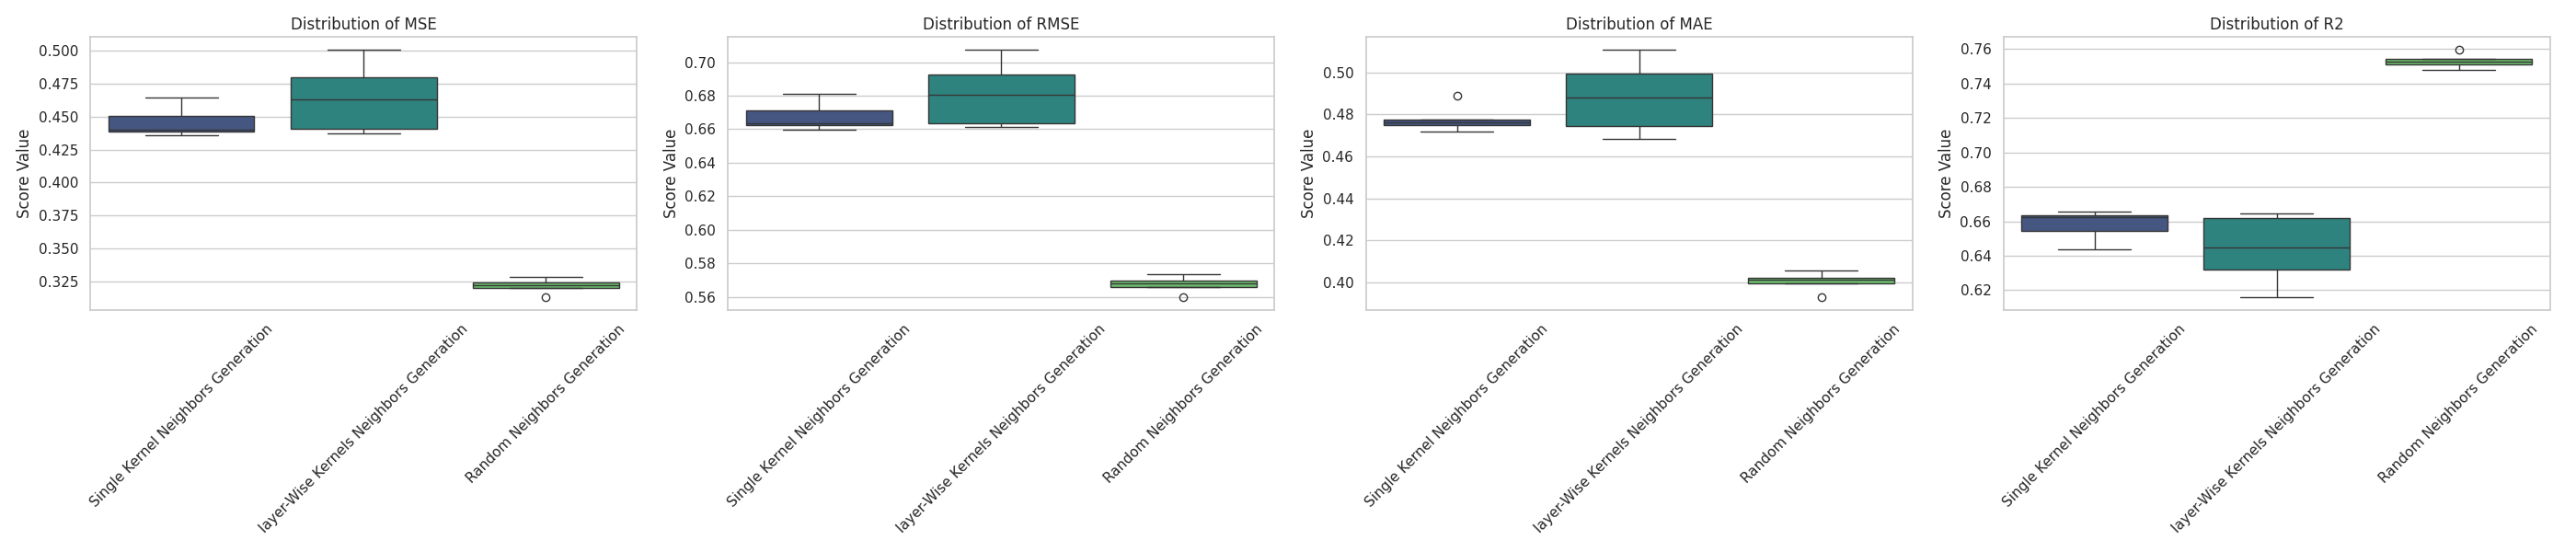
\includegraphics[width=1\textwidth]{figures/results/medium_net_neighbors_generation_strategies_comparison_no_BS/medium_net_neighbors_generation_strategies_comparison_no_BS_metrics_distribution.png}
    \caption{Regression metrics distribution across strategies for Medium Net.}
    \label{fig:medium_net_comp_metrics_dist}
\end{figure}

The metrics highlight a superior predictive capability for the Random sampling strategy, achieving an average $R^2$ of $0.7531$, compared to $0.6580$ and $0.6438$ for the Single and Layer-wise kernel methods, respectively. This confirms that stochastic neighbors provide a more robust exploration of the error surface for deeper networks.

\subsubsection{Summary Statistics}

Table \ref{tab:medium_net_comp_results} provides the numerical performance breakdown for the Medium Net.

\begin{table}[h]
\centering
\scriptsize
\begin{tabular}{|l|c|c|c|}
\hline
\textbf{Metric (Avg)} & \textbf{Random (0.01 / 0.1)} & \textbf{Single Kernel} & \textbf{Layer-wise Kernels} \\ \hline
Avg Final Loss        & 0.3076                       & 0.4364                 & 0.4529                      \\ \hline
Avg Time (s)          & 776.89                       & 727.95                 & 728.50                      \\ \hline
Avg MSE               & 0.3218                       & 0.4458                 & 0.4643                      \\ \hline
Avg RMSE              & 0.5672                       & 0.6676                 & 0.6812                      \\ \hline
Avg MAE               & 0.4002                       & 0.4780                 & 0.4883                      \\ \hline
Avg $R^2$             & 0.7531                       & 0.6580                 & 0.6438                      \\ \hline
\end{tabular}
\caption{Average statistical comparison of generation strategies for Medium Net.}
\label{tab:medium_net_comp_results}
\end{table}


\subsection{Big Net Results}

The Big Net architecture represents the most complex search space in this study. The three strategies were compared using the parameters found to be most effective for this scale:
\begin{itemize}
    \item \textbf{Single Kernel:} Weight kernel $[6,6]$, Bias kernel $[6]$, Stride 6.
    \item \textbf{Layer-wise Kernels:} 
        \begin{itemize}
            \item Weight kernels: $[[6,2], [6,6], [4,4], [4,4], [1,2]]$
            \item Bias kernels: $[[6], [6], [4], [2], [1]]$
            \item Weight strides: $[[2,6], [6,6], [4,4], [4,4], [2,1]]$
            \item Bias strides: $[[6], [6], [4], [2], [1]]$
        \end{itemize}
    \item \textbf{Random Sampling:} Perturbation ratio 0.1, Search coverage ratio 0.05.
\end{itemize}


\subsubsection{Visual Analysis of Training and Stability}

The convergence patterns for the Big Net, illustrated in Figure \ref{fig:big_net_comp_convergence}, confirm the trends observed in smaller networks but with higher absolute loss values due to the increased dimensionality.

\begin{figure}[htbp]
    \centering
    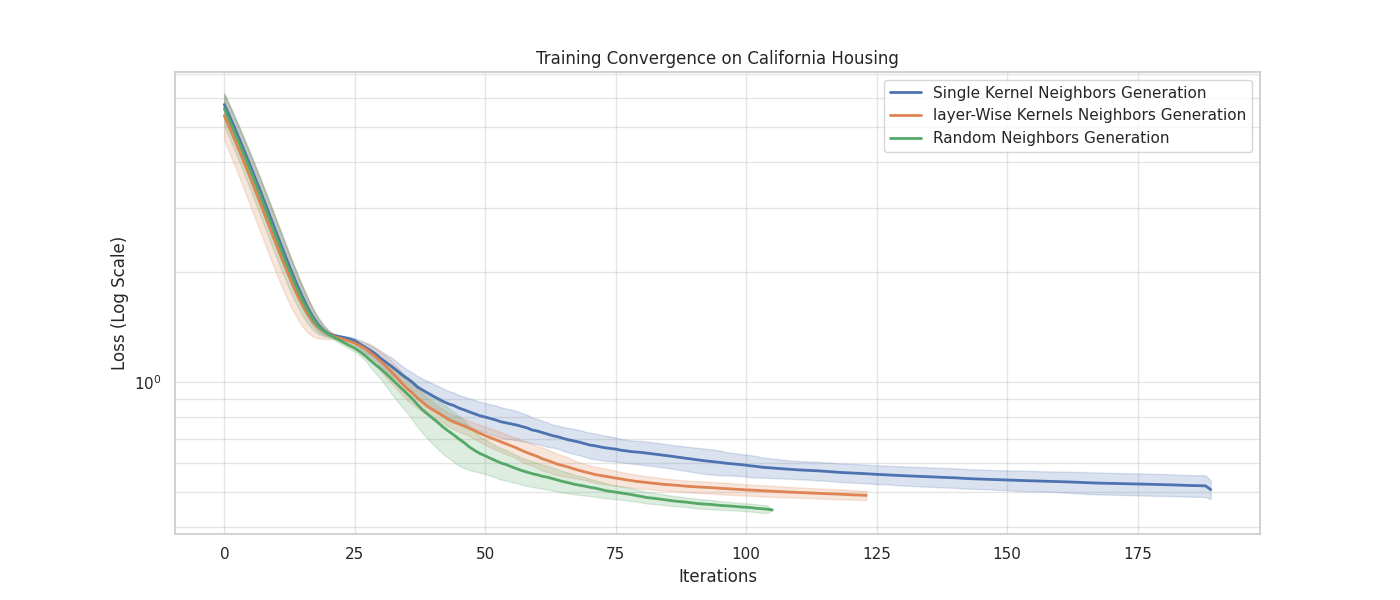
\includegraphics[width=0.9\textwidth]{figures/results/big_net_neighbors_generation_strategies_comparison_no_BS/big_net_neighbors_generation_strategies_comparison_no_BS_convergence.png}
    \caption{Training convergence comparison for Big Net (Log Scale).}
    \label{fig:big_net_comp_convergence}
\end{figure}

The \textit{Random Neighbors Generation} (green line) continues to be the most effective strategy, achieving a final loss significantly lower than its deterministic counterparts. In this high-parameter setting, the \textit{Single Kernel} method (blue line) shows the most difficulty in refining weights, plateauting at a higher loss value compared to the \textit{Layer-wise} approach.

The stability of these outcomes is summarized in the boxplot distribution in Figure \ref{fig:big_net_comp_final_loss}.

\newpage

\begin{figure}[htbp]
    \centering
    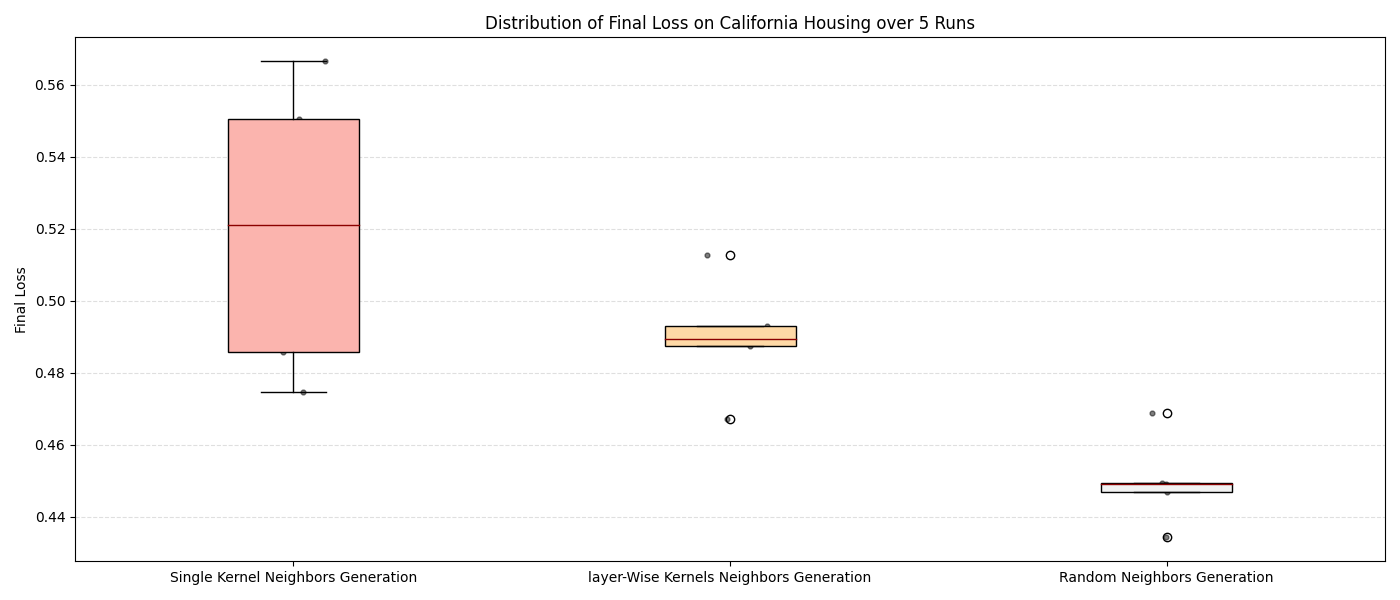
\includegraphics[width=0.85\textwidth]{figures/results/big_net_neighbors_generation_strategies_comparison_no_BS/big_net_neighbors_generation_strategies_comparison_no_BS_final_loss.png}
    \caption{Distribution of Final Loss for Big Net generation strategies.}
    \label{fig:big_net_comp_final_loss}
\end{figure}

The Random strategy exhibits the lowest average loss ($0.4497$) and the \\
lowest standard deviation ($0.0110$), indicating a high degree of reliability in high-dimensional spaces. While the \textit{Layer-wise} method outperforms the \textit{Single Kernel}, it still \\ 
remains nearly $9\%$ behind the Random strategy in terms of average final loss.

\newpage

Figure \ref{fig:big_net_comp_metrics_dist} displays the regression metrics across the three strategies for the Big Net.

\begin{figure}[htbp]
    \centering
    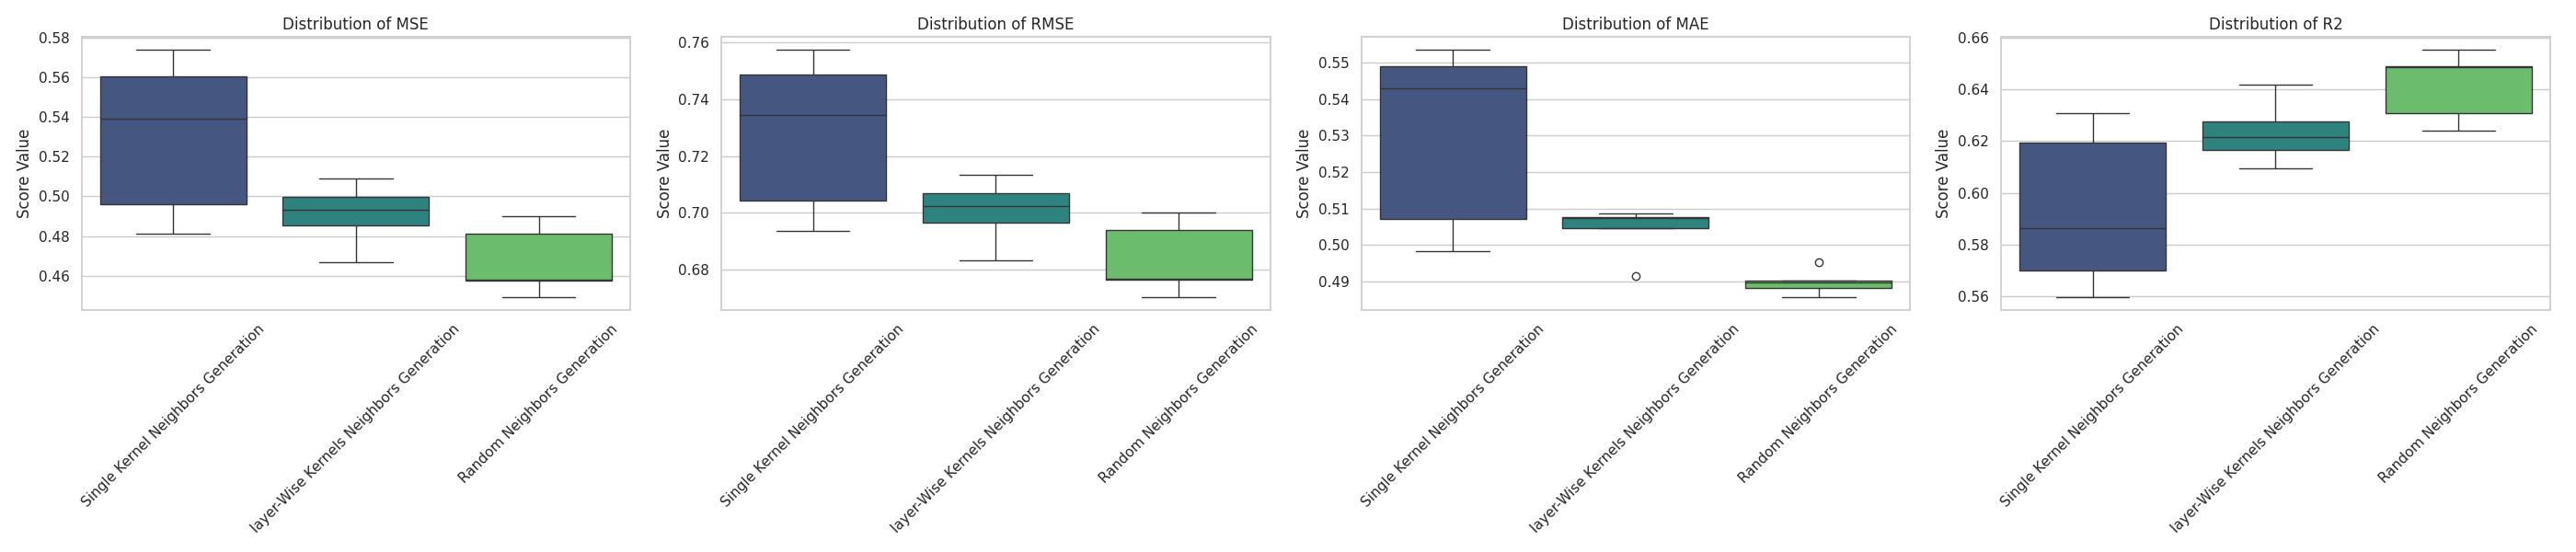
\includegraphics[width=1\textwidth]{figures/results/big_net_neighbors_generation_strategies_comparison_no_BS/big_net_neighbors_generation_strategies_comparison_no_BS_metrics_distribution.png}
    \caption{Regression metrics distribution across strategies for Big Net.}
    \label{fig:big_net_comp_metrics_dist}
\end{figure}

The $R^2$ scores demonstrate the scaling advantage of stochastic search: the Random strategy achieves an average $R^2$ of $0.6416$, whereas the Single Kernel approach struggles to maintain predictive power, dropping below $0.60$. This suggests that as network size increases, the flexibility of the neighbor generation becomes the primary factor in model performance.

\subsubsection{Summary Statistics}

Table \ref{tab:big_net_comp_results} provides the final average numerical comparison for the Big Net architecture.

\begin{table}[h]
\centering
\scriptsize
\begin{tabular}{|l|c|c|c|}
\hline
\textbf{Metric (Avg)} & \textbf{Random (0.1 / 0.05)} & \textbf{Single Kernel} & \textbf{Layer-wise Kernels} \\ \hline
Avg Final Loss        & 0.4497                       & 0.5197                 & 0.4899                      \\ \hline
Avg Time (s)          & 720.60                       & 703.09                 & 702.34                      \\ \hline
Avg MSE               & 0.4672                       & 0.5302                 & 0.4908                      \\ \hline
Avg RMSE              & 0.6834                       & 0.7277                 & 0.7005                      \\ \hline
Avg MAE               & 0.4898                       & 0.5302                 & 0.5040                      \\ \hline
Avg $R^2$             & 0.6416                       & 0.5932                 & 0.6234                      \\ \hline
\end{tabular}
\caption{Average statistical comparison of generation strategies for Big Net.}
\label{tab:big_net_comp_results}
\end{table}

\subsection{Conclusion on Neighbors Generation Strategies}

The comparative analysis across all three network architectures — Small, Medium, and Big Net — provides conclusive evidence regarding the effectiveness of the proposed neighbor generation strategies.

\begin{itemize}
    \item \textbf{Dominance of Random Sampling:} The results consistently demonstrate that the \textit{Random Neighbors Generation} approach is the most effective strategy for weight optimization in an $A^*$-based framework. Across all architectures, it yielded significantly lower final loss and Mean Squared Error (MSE) compared to kernel-based methods. For instance, in the Small Net, the Random strategy achieved an MSE of $0.3035$, nearly $25\%$ lower than the best kernel-based result ($0.4055$).
    
    \item \textbf{Limitations of Structural Kernels:} The \textit{Single Kernel} and \textit{Layer-wise} approaches produced comparable results that were consistently inferior to stochastic sampling. This suggests that the rigid structural constraints imposed by kernels (weights and biases updated in fixed blocks) limit the search algorithm's ability to navigate the complex, non-linear error surfaces of neural networks. In contrast, the stochastic nature of random sampling provides the flexibility needed to find more efficient descent directions.
    
    \item \textbf{Scalability and Predictive Power:} The superiority of the Random approach is further validated by the $R^2$ scores, which remained robust even as network complexity increased. While kernel-based methods saw a notable drop in predictive performance when transitioning to larger networks, the Random strategy maintained high $R^2$ values (e.g., $0.7531$ in Medium Net and $0.6416$ in Big Net), highlighting its superior scalability.
    
    \item \textbf{Kernel Evolution in Large Networks:} An interesting observation occurred in the \textbf{Big Net} architecture, where the \textit{Layer-wise} strategy finally outperformed the \textit{Single Kernel} approach. This indicates that as the parameter space expands, per-layer customization becomes more relevant for deterministic updates, although it still fails to bridge the performance gap with stochastic search.
\end{itemize}

In summary, the \textbf{Random Neighbors Generation} strategy is identified as the key driver for high-performance training in this study. Its ability to achieve superior convergence stability and predictive accuracy makes it the recommended choice for optimizing neural networks where traditional gradient descent is not applicable.

\newpage

%%%%%%%%%%%%%%%%%%%%%BEAM SEARCH OPTIMIZATION%%%%%%%%%%%%%%%%%%%%%%%%%
\section{Beam Search Optimization Study}
\label{sec:beam_search_study}

The final component of this preliminary study investigates the implementation of the \textbf{Beam Search} strategy as a solution to the critical limitation of main memory saturation. In a standard $A^*$ search, the Open and Closed sets grow exponentially, often leading to RAM exhaustion before an optimal solution is reached, especially in deep neural networks. 

By employing a Beam Search with a fixed \textbf{Beam Width (BW)}, the algorithm limits the number of states kept in memory at each search level. This experiment compares the performance of the classic (vanilla) $A^*$ training against three different beam widths ($100$, $1,000$, and $10,000$) to evaluate whether this memory-efficient approach can maintain optimization quality while preventing hardware-related interruptions.

\subsection{Small Net Results}

For the Small Net architecture, the test was conducted to establish a baseline for how Beam Search impacts optimization when memory saturation is not yet a critical factor. The following parameters were applied:

\begin{itemize}
    \item \textbf{Weight Kernel Size:} $[2,2]$, \textbf{Bias Kernel Size:} $[2]$, \textbf{Strides:} 2.
    \item \textbf{Quantization Factor:} 10 (Static).
    \item \textbf{Beam Widths tested:} $100, 1,000, 10,000$.
    \item \textbf{Runs:} 5 for each configuration.
\end{itemize}

\newpage

\subsubsection{Visual Analysis of Training and Stability}

The convergence trajectories for the Small Net are shown in Figure \ref{fig:small_net_bs_convergence}. Given the relatively small state-space of this network, all configurations follow a nearly identical path toward convergence.

\begin{figure}[htbp]
    \centering
    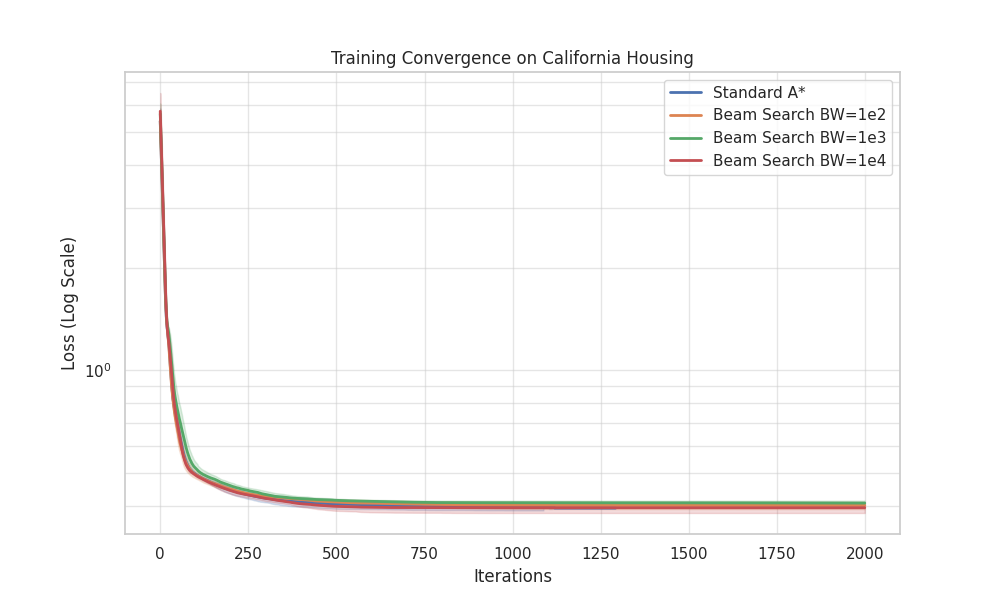
\includegraphics[width=0.9\textwidth]{figures/results/small_net_vanilla_train_vs_beam_search/small_net_vanilla_train_vs_beam_search_convergence.png}
    \caption{Training convergence comparison: Standard A* vs. various Beam Widths (Log Scale).}
    \label{fig:small_net_bs_convergence}
\end{figure}

The \textit{Standard A*} and \textit{Beam Search BW=10,000} show the most overlap, indicating that a sufficiently wide beam width can effectively approximate the full search space for smaller models.

\newpage

Figure \ref{fig:small_net_bs_final_loss} displays the distribution of final loss values. It is observed that as the Beam Width increases, the final loss values tend to consolidate and improve.

\begin{figure}[htbp]
    \centering
    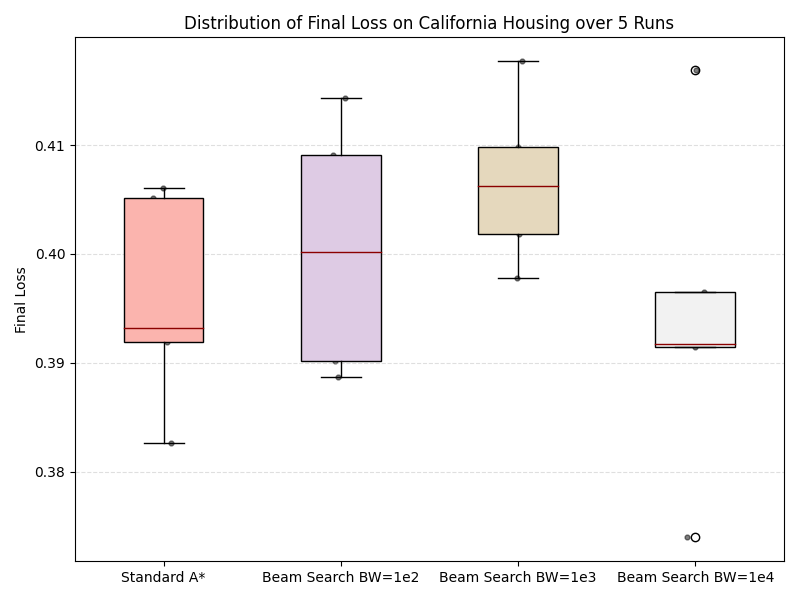
\includegraphics[width=0.85\textwidth]{figures/results/small_net_vanilla_train_vs_beam_search/small_net_vanilla_train_vs_beam_search_final_loss.png}
    \caption{Distribution of Final Loss for Standard A* and Beam Search configurations.}
    \label{fig:small_net_bs_final_loss}
\end{figure}

Interestingly, the Standard $A^*$ exhibits a wider variance in the Small Net compared to the $BW=10,000$ configuration, suggesting that the pruning mechanism of Beam Search might occasionally filter out high-variance paths that Standard $A^*$ would otherwise explore.

\newpage

The regression metrics for the Small Net are summarized in Figure \ref{fig:small_net_bs_metrics_dist}.

\begin{figure}[htbp]
    \centering
    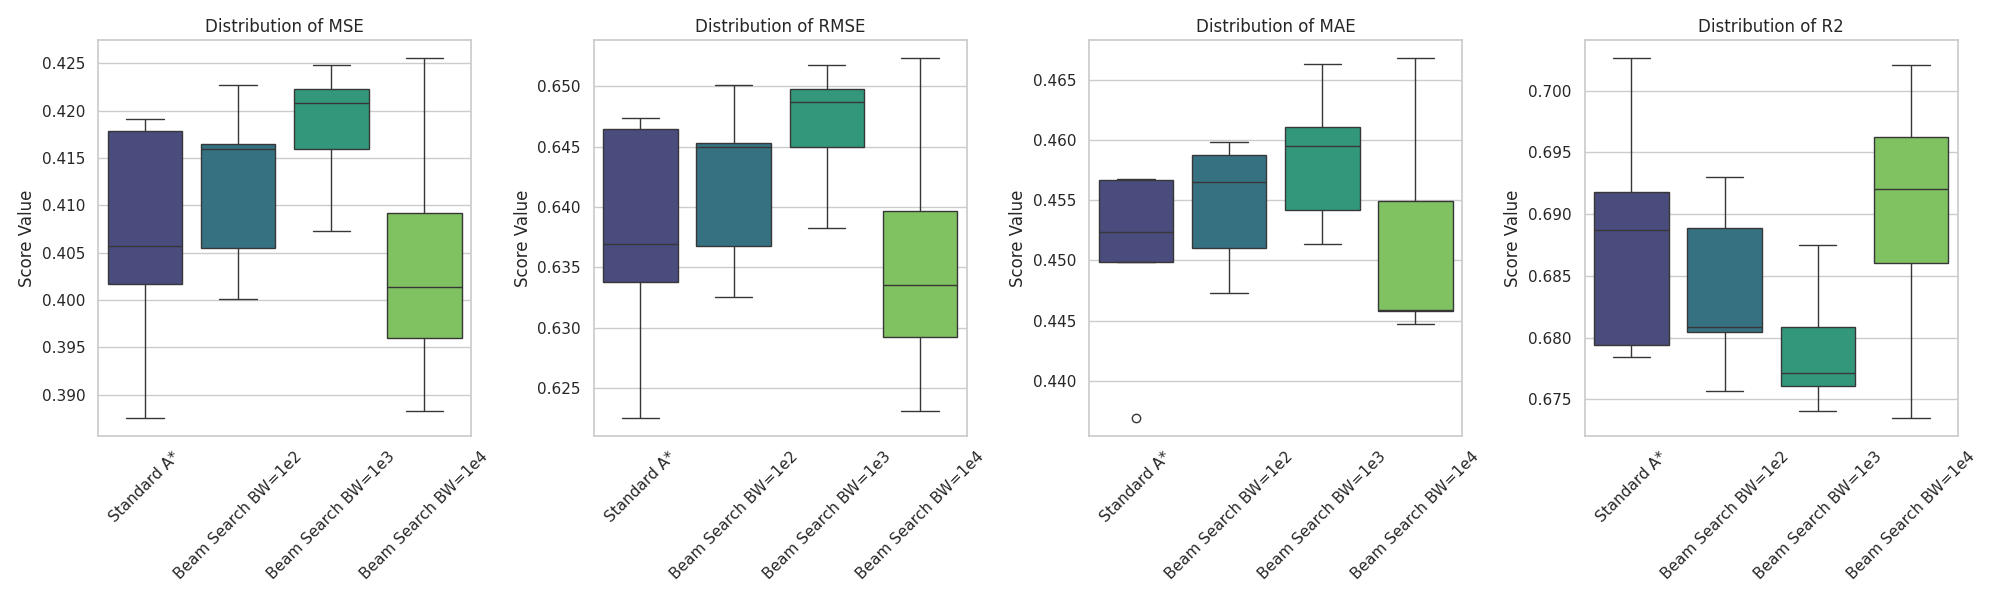
\includegraphics[width=1\textwidth]{figures/results/small_net_vanilla_train_vs_beam_search/small_net_vanilla_train_vs_beam_search_metrics_distribution.png}
    \caption{Regression metrics distribution across Beam Search configurations for Small Net.}
    \label{fig:small_net_bs_metrics_dist}
\end{figure}

The average $R^2$ values remain extremely stable across all tests, hovering around $0.68$-$0.69$. This confirms that for architectures of this size, implementing Beam Search does not significantly compromise the model's ability to model the California Housing data.

\subsubsection{Summary Statistics}

Table \ref{tab:small_net_bs_results} provides the numerical breakdown of the performance, highlighting the trade-off between search complexity and computational time.

\begin{table}[h]
\centering
\scriptsize
\begin{tabular}{|l|c|c|c|c|}
\hline
\textbf{Metric (Avg)} & \textbf{Standard A*} & \textbf{BW=1e2} & \textbf{BW=1e3} & \textbf{BW=1e4} \\ \hline
Avg Final Loss        & 0.3958               & 0.4005          & 0.4067          & 0.3941          \\ \hline
Avg Time (s)          & 772.46               & 1485.36         & 1514.21         & 1679.42         \\ \hline
Avg MSE               & 0.4064               & 0.4121          & 0.4182          & 0.4041          \\ \hline
Avg RMSE              & 0.6374               & 0.6420          & 0.6467          & 0.6356          \\ \hline
Avg MAE               & 0.4505               & 0.4547          & 0.4585          & 0.4516          \\ \hline
Avg $R^2$             & 0.6882               & 0.6838          & 0.6791          & 0.6900          \\ \hline
\end{tabular}
\caption{Average statistical comparison: Standard A* vs. Beam Search for Small Net.}
\label{tab:small_net_bs_results}
\end{table}

\newpage

\subsection{Medium Net Results}

The evaluation of the Beam Search strategy was extended to the Medium Net architecture to observe the trade-offs between memory management and optimization efficiency in a higher-dimensional state space. The experimental parameters remained consistent with the Small Net tests:

\begin{itemize}
    \item \textbf{Weight Kernel Size:} $[4,4]$, \textbf{Bias Kernel Size:} $[4]$, \textbf{Strides:} 4.
    \item \textbf{Quantization Factor:} 10 (Static).
    \item \textbf{Beam Widths tested:} $100, 1,000, 10,000$.
    \item \textbf{Runs:} 5 for each configuration.
\end{itemize}

\subsubsection{Visual Analysis of Training and Stability}

The convergence patterns for the Medium Net, illustrated in Figure \ref{fig:medium_net_bs_convergence}, show a remarkable degree of overlap across all configurations. 

\begin{figure}[htbp]
    \centering
    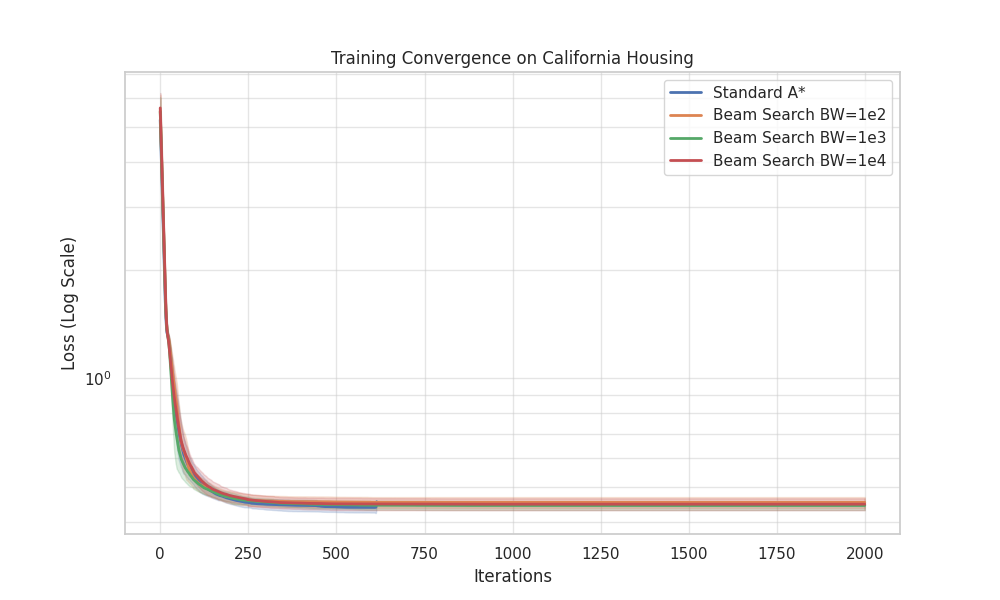
\includegraphics[width=0.9\textwidth]{figures/results/medium_net_vanilla_train_vs_beam_search/medium_net_vanilla_train_vs_beam_search_convergence.png}
    \caption{Training convergence comparison for Medium Net: Standard A* vs. various Beam Widths (Log Scale).}
    \label{fig:medium_net_bs_convergence}
\end{figure}

Even with the increased complexity of the Medium Net, the pruning mechanism of the Beam Search does not prevent the algorithm from following a convergence trajectory nearly identical to the Standard $A^*$ search. This indicates that the most promising descent directions are correctly preserved within the beam, even at a width of $100$.

Figure \ref{fig:medium_net_bs_final_loss} displays the distribution of final loss values. The results suggest that the Standard $A^*$ and the wider Beam Width ($BW=10,000$) maintain the most consistent loss profiles.

\begin{figure}[htbp]
    \centering
    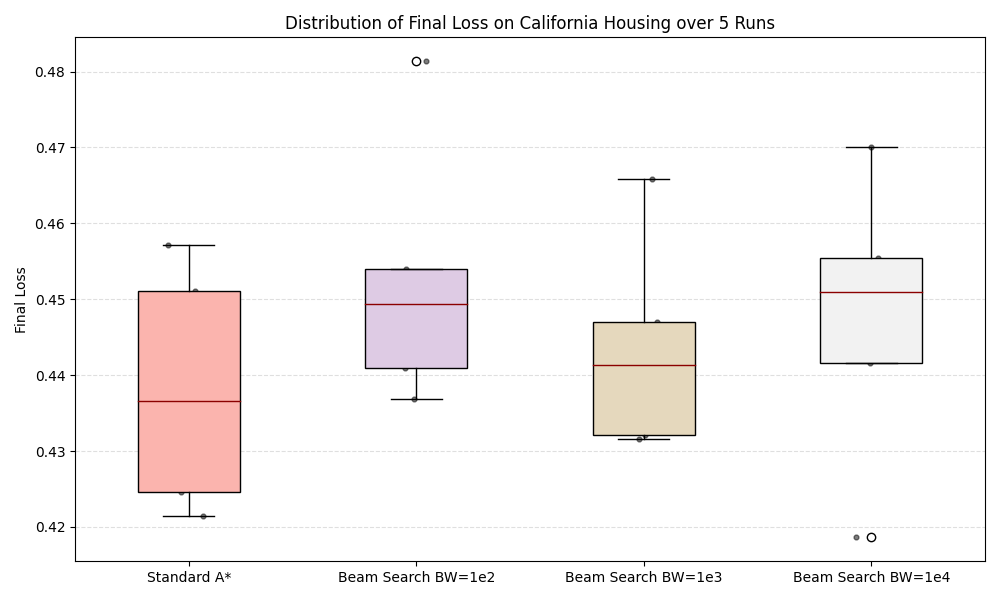
\includegraphics[width=0.85\textwidth]{figures/results/medium_net_vanilla_train_vs_beam_search/medium_net_vanilla_train_vs_beam_search_final_loss.png}
    \caption{Distribution of Final Loss for Medium Net across Beam Search configurations.}
    \label{fig:medium_net_bs_final_loss}
\end{figure}

While the Average Final Loss for $BW=100$ ($0.4525$) is slightly higher than the Standard $A^*$ ($0.4382$), the difference is marginal, confirming that Beam Search is a viable alternative for larger networks where memory limitations become a bottleneck.

\newpage

The predictive accuracy metrics for the Medium Net are visualized in Figure \ref{fig:medium_net_bs_metrics_dist}.

\begin{figure}[htbp]
    \centering
    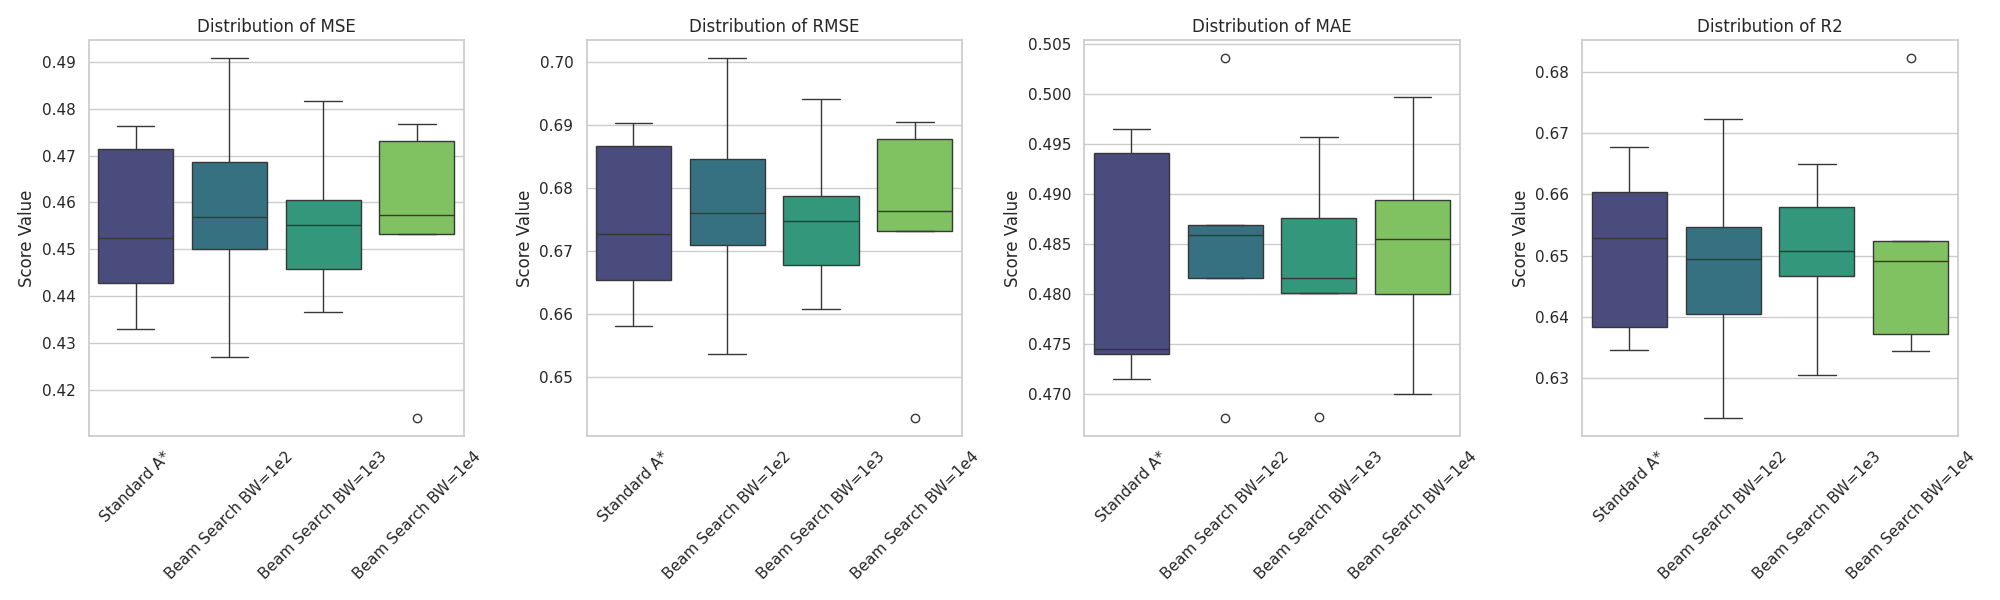
\includegraphics[width=1\textwidth]{figures/results/medium_net_vanilla_train_vs_beam_search/medium_net_vanilla_train_vs_beam_search_metrics_distribution.png}
    \caption{Regression metrics distribution across Beam Search configurations for Medium Net.}
    \label{fig:medium_net_bs_metrics_dist}
\end{figure}

The metrics confirm that optimization quality is preserved despite the state-space pruning. The average $R^2$ values remain remarkably consistent, with the $BW=10,000$ configuration achieving an average $R^2$ of $0.6510$, virtually identical to the $0.6508$ achieved by the Standard $A^*$ search.

\subsubsection{Summary Statistics}

Table \ref{tab:medium_net_bs_results} provides the numerical performance summary, highlighting the significant time disparity between the classic search and the beam-limited search.

\begin{table}[h]
\centering
\scriptsize
\begin{tabular}{|l|c|c|c|c|}
\hline
\textbf{Metric (Avg)} & \textbf{Standard A*} & \textbf{BW=1e2} & \textbf{BW=1e3} & \textbf{BW=1e4} \\ \hline
Avg Final Loss        & 0.4382               & 0.4525          & 0.4436          & 0.4473          \\ \hline
Avg Time (s)          & 730.16               & 2682.06         & 2888.02         & 3332.55         \\ \hline
Avg MSE               & 0.4552               & 0.4587          & 0.4560          & 0.4549          \\ \hline
Avg RMSE              & 0.6746               & 0.6771          & 0.6752          & 0.6742          \\ \hline
Avg MAE               & 0.4822               & 0.4851          & 0.4826          & 0.4849          \\ \hline
Avg $R^2$             & 0.6508               & 0.6481          & 0.6502          & 0.6510          \\ \hline
\end{tabular}
\caption{Average statistical comparison: Standard A* vs. Beam Search for Medium Net.}
\label{tab:medium_net_bs_results}
\end{table}

\newpage

\subsection{Big Net Results}

The evaluation of the Beam Search strategy on the Big Net architecture represents the most significant test case for memory management. With a considerably larger state space, the Standard $A^*$ algorithm is prone to premature termination due to RAM saturation. The experimental parameters were configured as follows:

\begin{itemize}
    \item \textbf{Weight Kernel Size:} $[8,8]$, \textbf{Bias Kernel Size:} $[8]$, \textbf{Strides:} 8.
    \item \textbf{Quantization Factor:} 10 (Static).
    \item \textbf{Beam Widths tested:} $100, 1,000, 10,000$.
    \item \textbf{Runs:} 5 for each configuration.
\end{itemize}

\subsubsection{Visual Analysis of Training and Stability}

The convergence trajectories for the Big Net are illustrated in Figure \ref{fig:big_net_bs_convergence}. In this complex architecture, the trajectories remain tightly clustered, indicating that the pruning of the search space does not adversely affect the primary descent path.

\begin{figure}[htbp]
    \centering
    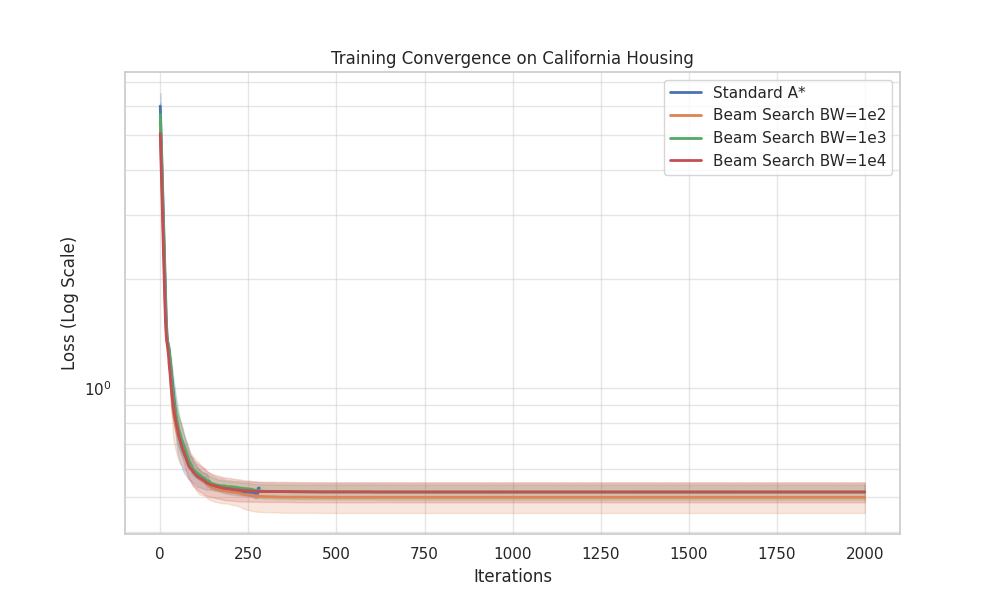
\includegraphics[width=0.9\textwidth]{figures/results/big_net_vanilla_train_vs_beam_search/big_net_vanilla_train_vs_beam_search_convergence.png}
    \caption{Training convergence comparison for Big Net: Standard A* vs. various Beam Widths (Log Scale).}
    \label{fig:big_net_bs_convergence}
\end{figure}

A critical observation is found in the execution time. The \textit{Standard A*} completes its execution in significantly less time ($\approx 691$s) compared to the Beam Search variants ($\approx 5300$-$6200$s). This disparity is likely due to the vanilla method reaching hardware memory limits rapidly and halting, whereas Beam Search manages the sets to allow for a more sustained optimization process.

The distribution of final loss values is shown in Figure \ref{fig:big_net_bs_final_loss}.

\begin{figure}[htbp]
    \centering
    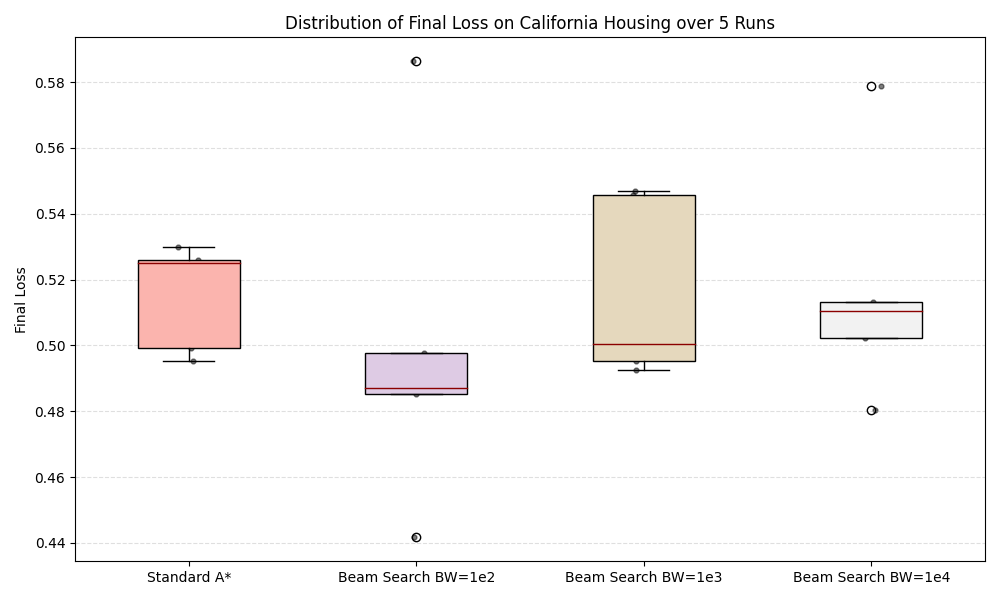
\includegraphics[width=0.85\textwidth]{figures/results/big_net_vanilla_train_vs_beam_search/big_net_vanilla_train_vs_beam_search_final_loss.png}
    \caption{Distribution of Final Loss for Big Net across Beam Search configurations.}
    \label{fig:big_net_bs_final_loss}
\end{figure}

Counter-intuitively, the \textbf{Beam Search with BW=100} achieved the lowest average final loss ($0.4996$), even lower than the Standard $A^*$ ($0.5150$). This suggests that for very large networks, aggressive pruning may act as a helpful constraint, preventing the algorithm from exploring high-cost branches that do not lead to a global minimum.

\newpage

The regression metrics for the Big Net are visualized in Figure \ref{fig:big_net_bs_metrics_dist}.

\begin{figure}[htbp]
    \centering
    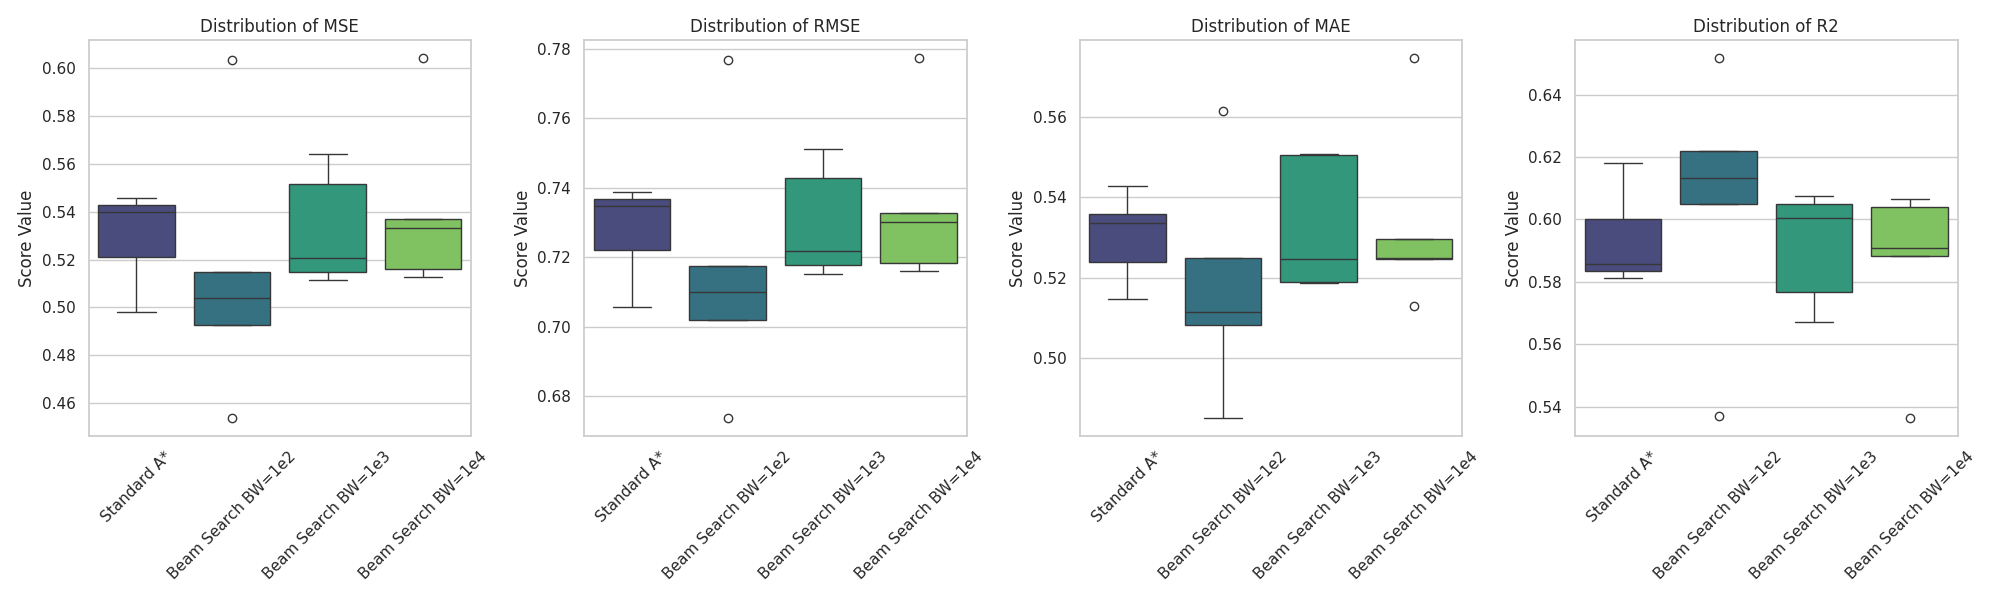
\includegraphics[width=1\textwidth]{figures/results/big_net_vanilla_train_vs_beam_search/big_net_vanilla_train_vs_beam_search_metrics_distribution.png}
    \caption{Regression metrics distribution across Beam Search configurations for Big Net.}
    \label{fig:big_net_bs_metrics_dist}
\end{figure}

The metrics confirm that the predictive quality remains consistent across different beam widths. The $R^2$ scores are centered around $0.59$-$0.60$. Remarkably, $BW=100$ yielded the highest average $R^2$ ($0.6058$), confirming that limiting the search set size is not only beneficial for memory management but can also improve general performance in high-dimensional spaces.

\subsubsection{Summary Statistics}

Table \ref{tab:big_net_bs_results} provides the numerical performance summary for the Big Net.

\begin{table}[h]
\centering
\scriptsize
\begin{tabular}{|l|c|c|c|c|}
\hline
\textbf{Metric (Avg)} & \textbf{Standard A*} & \textbf{BW=1e2} & \textbf{BW=1e3} & \textbf{BW=1e4} \\ \hline
Avg Final Loss        & 0.5150               & 0.4996          & 0.5161          & 0.5170          \\ \hline
Avg Time (s)          & 691.68               & 5369.14         & 5681.63         & 6267.84         \\ \hline
Avg MSE               & 0.5295               & 0.5137          & 0.5326          & 0.5406          \\ \hline
Avg RMSE              & 0.7276               & 0.7160          & 0.7297          & 0.7349          \\ \hline
Avg MAE               & 0.5302               & 0.5182          & 0.5327          & 0.5333          \\ \hline
Avg $R^2$             & 0.5937               & 0.6058          & 0.5914          & 0.5852          \\ \hline
\end{tabular}
\caption{Average statistical comparison: Standard A* vs. Beam Search for Big Net.}
\label{tab:big_net_bs_results}
\end{table}

\newpage

\subsection{Conclusion on Beam Search Optimization Study}

The comparative analysis between the Standard $A^*$ algorithm and the Beam Search strategy provides critical insights into resource management and optimization persistence for neural network training.

\begin{itemize}
    \item \textbf{Resolution of Memory Constraints:} The primary and most significant finding is that Beam Search effectively resolves the hardware limitations associated with Standard $A^*$. In every architecture tested, the Standard $A^*$ search failed to reach the maximum limit of 2,000 iterations, as the exponential growth of the Open and Closed sets led to complete RAM saturation. In contrast, all Beam Search configurations successfully completed the full 2,000-iteration cycle, confirming its necessity for stable, long-term optimization.
    
    \item \textbf{Consistent Performance Gains:} Across all tested networks, the Beam Search strategy consistently outperformed the vanilla training method, albeit by a marginal lead. The most notable improvement was observed in the \textbf{Big Net}, where the most aggressive pruning (BW=100) achieved the highest $R^2$ score ($0.6058$) and the lowest average loss ($0.4996$). This suggests that limiting the search breadth may act as a regularizer, forcing the algorithm to prioritize the most promising paths identified by the heuristic function.
    
    \item \textbf{Efficiency of Narrow Beam Widths:} The data indicates that a wide beam is not always necessary for high-quality results. Even with a narrow Beam Width of $100$, the algorithm maintained a predictive accuracy comparable to or better than the full search. This highlights the effectiveness of the underlying heuristic in correctly ordering neighbors, allowing for the disposal of the vast majority of search nodes without losing the optimal descent direction.
    
    \item \textbf{Computational Trade-off:} While Beam Search ensures memory stability, it introduces a significant computational overhead due to the sorting and pruning logic required at each step. This resulted in execution times that were significantly higher than those of the Standard $A^*$ runs. However, since the vanilla method’s shorter time is a direct consequence of premature termination due to memory failure, the increased duration of Beam Search is a necessary cost for achieving a complete and deeper optimization.
\end{itemize}

In conclusion, the \textbf{Beam Search} strategy is a fundamental optimization for the $A^*$-based training framework. By transforming an unbounded search into a resource-constrained process, it allows for the training of larger architectures that would otherwise be impossible to optimize using traditional search methods.

%%%%%%%%%%%%% NEIGHBOR GENERATION STRATEGIES WITH BEAM SEARCH %%%%%%%%%%%%%%%%%%%%%%%
\section{Neighbors Generation Strategies Comparison with Beam Search}
\label{sec:strategies_comparison_bs}

In this phase of the preliminary study, the three neighbor generation strategies \\
—\textit{Single Kernel}, \textit{Layer-wise Kernels}, and \textit{Random Neighbors Generation}—are compared while activating the \textbf{Beam Search} optimization. The objective is to determine if the synergies between memory-limited search and stochastic or deterministic generation methods lead to superior convergence profiles on the California Housing dataset.

Unless otherwise specified, all tests maintain the optimal hyperparameters identified in earlier sections and use a static quantization factor of 10.

\subsection{Small Net Results}

The Small Net architecture was evaluated using the following configurations with Beam Search active:
\begin{itemize}
    \item \textbf{Single Kernel:} Weight kernel $[2,2]$, Bias kernel $[2]$, Stride 2.
    \item \textbf{Layer-wise Kernels:} 
        \begin{itemize}
            \item Weight kernels: $[[2,2], [2,2], [1,2]]$
            \item Bias kernels: $[[2], [2], [1]]$
            \item Weight strides: $[[2,2], [2,2], [2,1]]$
            \item Bias strides: $[[2], [2], [1]]$
        \end{itemize}
    \item \textbf{Random Sampling:} Perturbation ratio 0.01, Search coverage ratio 0.1.
\end{itemize}

\newpage

\subsubsection{Visual Analysis of Training and Stability}

The training convergence for the Small Net with Beam Search is illustrated in Figure \ref{fig:small_net_comp_bs_convergence}. 

\begin{figure}[htbp]
    \centering
    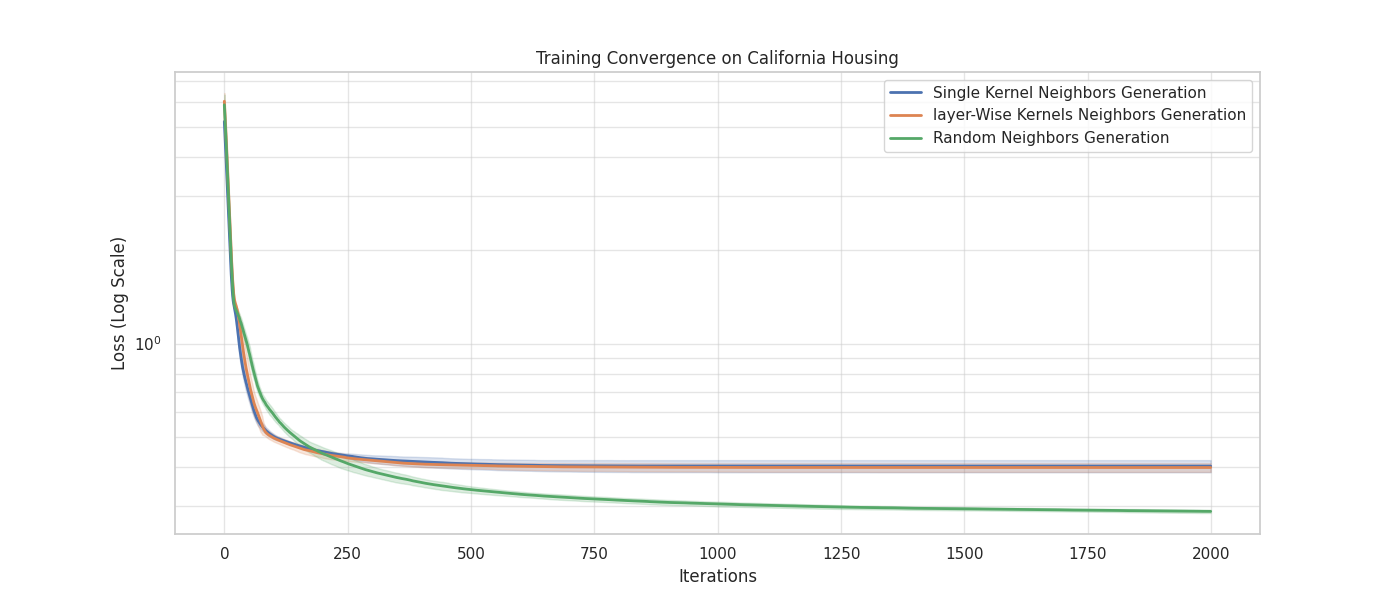
\includegraphics[width=0.9\textwidth]{figures/results/small_net_neighbors_generation_strategies_comparison_with_BS/small_net_neighbors_generation_strategies_comparison_with_BS_convergence.png}
    \caption{Training convergence comparison for Small Net with Beam Search (Log Scale).}
    \label{fig:small_net_comp_bs_convergence}
\end{figure}

The activation of Beam Search preserves the performance hierarchy established in previous tests. The \textit{Random Neighbors Generation} (green line) demonstrates a superior ability to find high-quality descent directions, achieving a final loss state significantly lower than the deterministic kernel-based methods. Both kernel strategies converge to a similar plateau early in the training process, indicating that the rigid geometric updates struggle to refine the solution further within the beam's constraints.

The stability of these outcomes is summarized in the boxplot distribution in Figure \ref{fig:small_net_comp_bs_final_loss}.

\newpage

\begin{figure}[htbp]
    \centering
    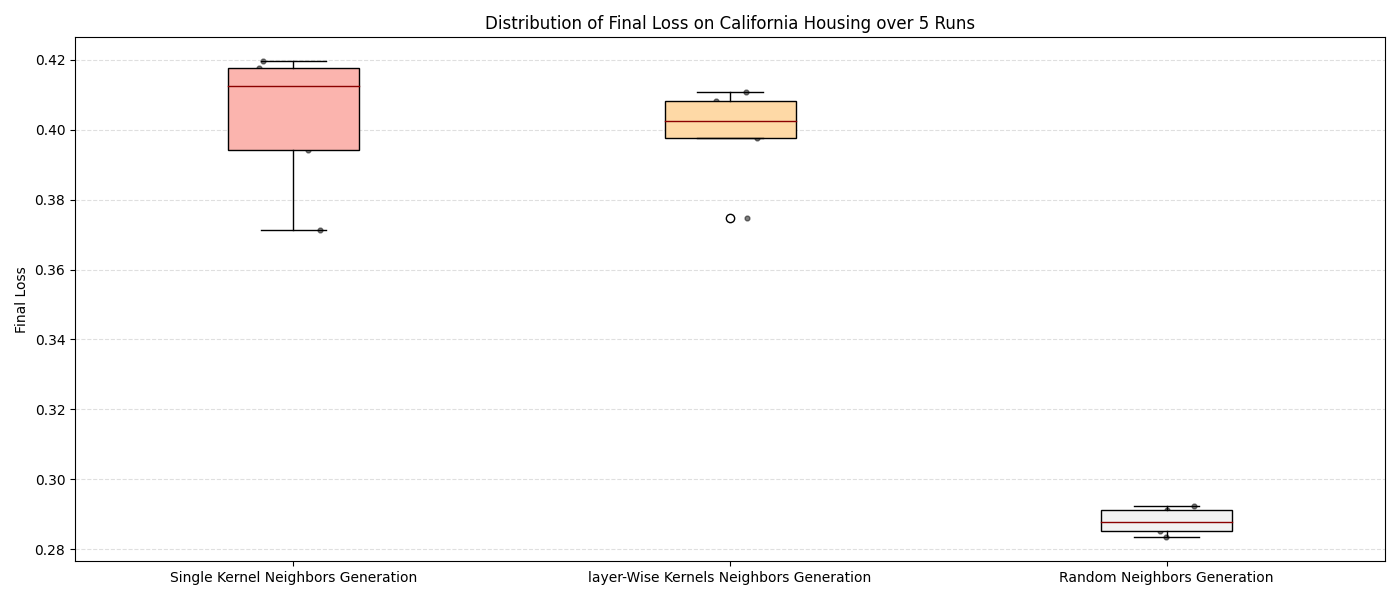
\includegraphics[width=0.85\textwidth]{figures/results/small_net_neighbors_generation_strategies_comparison_with_BS/small_net_neighbors_generation_strategies_comparison_with_BS_final_loss.png}
    \caption{Distribution of Final Loss with Beam Search for Small Net.}
    \label{fig:small_net_comp_bs_final_loss}
\end{figure}

The \textit{Random Neighbors Generation} strategy maintains the lowest average final loss ($0.2880$) and the most stable distribution. In contrast, the \textit{Single Kernel} approach exhibits higher variance and the highest average final loss ($0.4031$), suggesting that without per-layer customization, the beam search often explores less productive paths compared to the stochastic alternative.

\newpage

The regression metrics for the Small Net with Beam Search are summarized in Figure \ref{fig:small_net_comp_bs_metrics_dist}.

\begin{figure}[htbp]
    \centering
    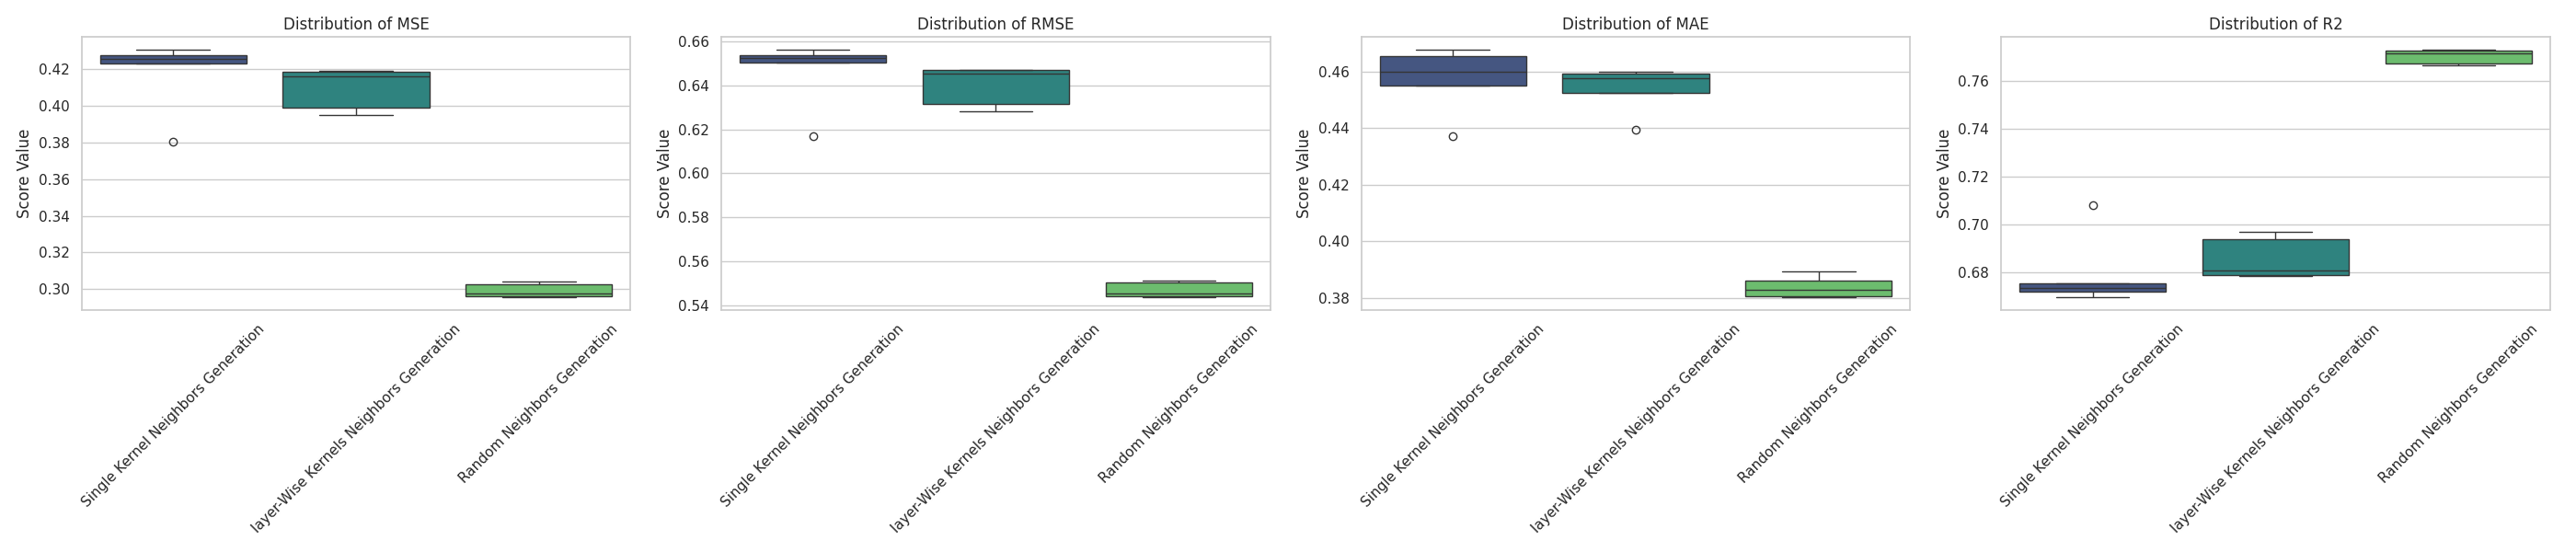
\includegraphics[width=1\textwidth]{figures/results/small_net_neighbors_generation_strategies_comparison_with_BS/small_net_neighbors_generation_strategies_comparison_with_BS_metrics_distribution.png}
    \caption{Regression metrics distribution across strategies for Small Net with Beam Search.}
    \label{fig:small_net_comp_bs_metrics_dist}
\end{figure}

The $R^2$ values highlight a clear performance gap: the Random strategy achieves an average score of $0.7704$, outperforming the Single Kernel ($0.6797$) and Layer-wise ($0.6858$) methods by nearly 10 percentage points. This confirms that the pruning logic of Beam Search is highly effective when paired with stochastic sampling, as it focuses computational resources on the most promising random perturbations.

\subsubsection{Summary Statistics}

Table \ref{tab:small_net_comp_bs_results} provides the numerical performance breakdown for the Small Net.

\begin{table}[h]
\centering
\scriptsize
\begin{tabular}{|l|c|c|c|}
\hline
\textbf{Metric (Avg)} & \textbf{Random (0.01 / 0.1)} & \textbf{Single Kernel} & \textbf{Layer-wise Kernels} \\ \hline
Avg Final Loss        & 0.2880                       & 0.4031                 & 0.3988                      \\ \hline
Avg Time (s)          & 624.23                       & 1430.77                & 1308.16                     \\ \hline
Avg MSE               & 0.2992                       & 0.4175                 & 0.4095                      \\ \hline
Avg RMSE              & 0.5470                       & 0.6460                 & 0.6399                      \\ \hline
Avg MAE               & 0.3839                       & 0.4571                 & 0.4537                      \\ \hline
Avg $R^2$             & 0.7704                       & 0.6797                 & 0.6858                      \\ \hline
\end{tabular}
\caption{Average statistical comparison of generation strategies with Beam Search for Small Net.}
\label{tab:small_net_comp_bs_results}
\end{table}

\newpage

\subsection{Medium Net Results}

L'architettura Medium Net è stata analizzata attivando la Beam Search e utilizzando le configurazioni ottimali precedentemente identificate. Per questo test, i parametri strutturali sono stati definiti come segue:

\begin{itemize}
    \item \textbf{Single Kernel:} Weight kernel $[4,4]$, Bias kernel $[4]$, Stride 4.
    \item \textbf{Layer-wise Kernels:} 
        \begin{itemize}
            \item Weight kernels: $[[4,4], [4,4], [4,4], [1,4]]$
            \item Bias kernels: $[[4], [4], [4], [1]]$
            \item Weight strides: $[[4,4], [4,4], [4,4], [4,1]]$
            \item Bias strides: $[[4], [4], [4], [1]]$
        \end{itemize}
    \item \textbf{Random Sampling:} Perturbation ratio 0.01, Search coverage ratio 0.05.
\end{itemize}

\newpage

\subsubsection{Visual Analysis of Training and Stability}

La Figura \ref{fig:medium_net_comp_bs_convergence} mostra il confronto della convergenza per le tre strategie applicate alla Medium Net con l'ausilio della Beam Search.

\begin{figure}[htbp]
    \centering
    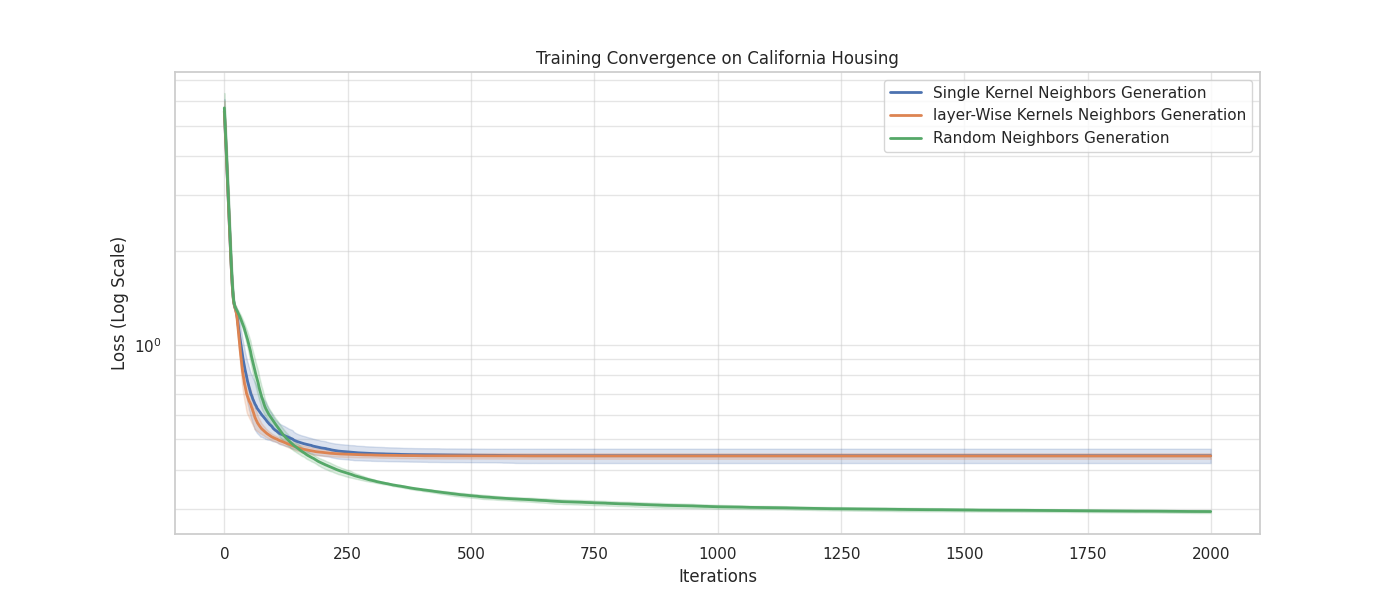
\includegraphics[width=0.9\textwidth]{figures/results/medium_net_neighbors_generation_strategies_comparison_with_BS/medium_net_neighbors_generation_strategies_comparison_with_BS_convergence.png}
    \caption{Confronto della convergenza per Medium Net con Beam Search (Scala Logaritmica).}
    \label{fig:medium_net_comp_bs_convergence}
\end{figure}

Analogamente a quanto osservato nella Small Net, la strategia \textit{Random Neighbors Generation} (linea verde) mantiene un vantaggio competitivo netto, stabilizzandosi su un livello di loss molto più basso rispetto ai metodi basati su kernel. Le strategie \textit{Single Kernel} e \textit{Layer-wise} mostrano un comportamento quasi identico, raggiungendo rapidamente un plateau che non riescono a superare nonostante l'ottimizzazione della memoria.

La distribuzione della loss finale è visualizzata nel boxplot della Figura \ref{fig:medium_net_comp_bs_final_loss}.

\newpage

\begin{figure}[htbp]
    \centering
    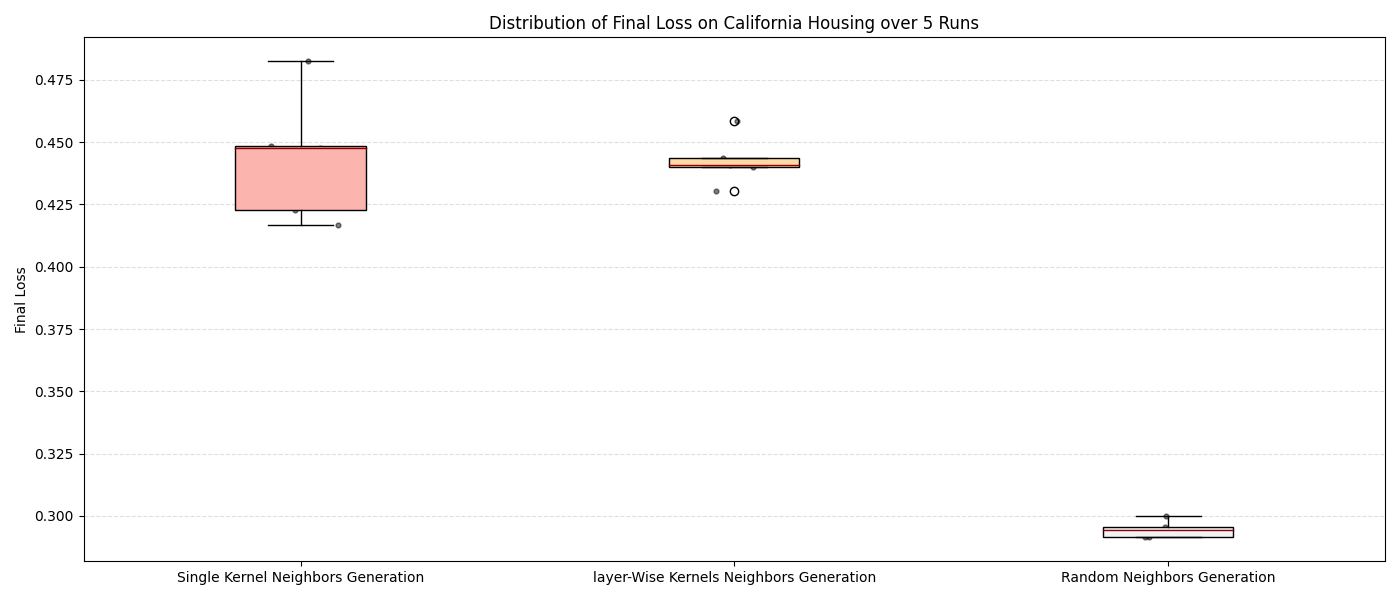
\includegraphics[width=0.85\textwidth]{figures/results/medium_net_neighbors_generation_strategies_comparison_with_BS/medium_net_neighbors_generation_strategies_comparison_with_BS_final_loss.png}
    \caption{Distribuzione della Loss Finale con Beam Search per Medium Net.}
    \label{fig:medium_net_comp_bs_final_loss}
\end{figure}

Il metodo Random conferma la sua robustezza con una loss media di $0.2945$ e una varianza estremamente ridotta ($0.000010$). È interessante notare come la Beam Search aiuti a mantenere i risultati del metodo \textit{Single Kernel} ($0.4437$) e \textit{Layer-wise} ($0.4428$) molto vicini tra loro, sebbene entrambi rimangano distanti dalle performance del campionamento stocastico.

\newpage

\subsubsection{Metrics Distribution and Predictive Performance}

Le metriche di regressione per la Medium Net con Beam Search sono riassunte nella Figura \ref{fig:medium_net_comp_bs_metrics_dist}.

\begin{figure}[htbp]
    \centering
    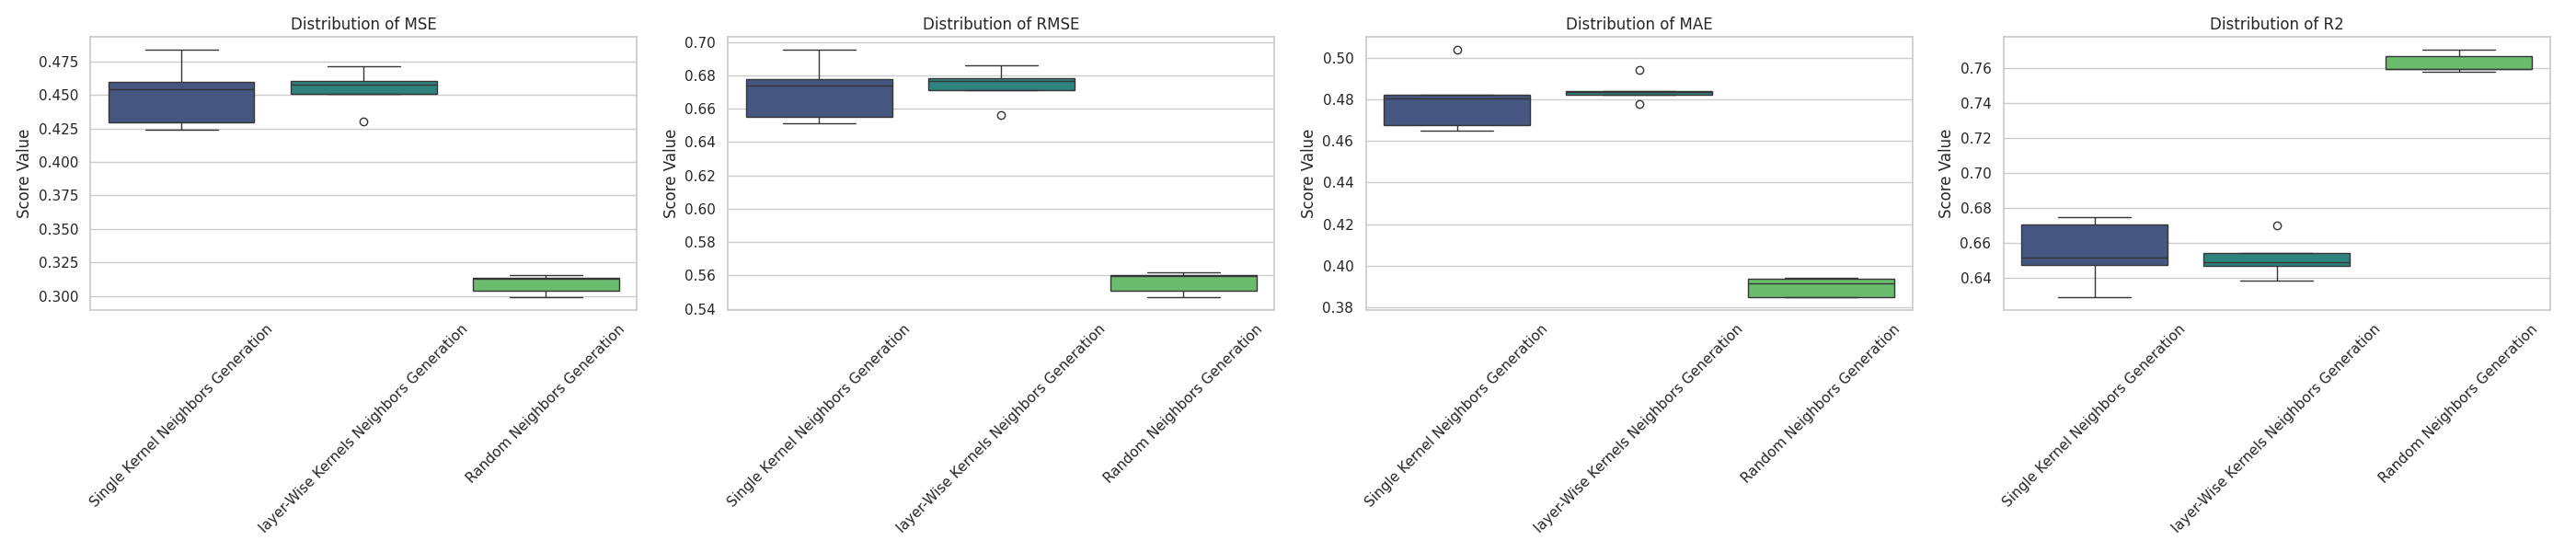
\includegraphics[width=1\textwidth]{figures/results/medium_net_neighbors_generation_strategies_comparison_with_BS/medium_net_neighbors_generation_strategies_comparison_with_BS_metrics_distribution.png}
    \caption{Distribuzione delle metriche di regressione con Beam Search per Medium Net.}
    \label{fig:medium_net_comp_bs_metrics_dist}
\end{figure}

Il valore medio di $R^2$ per il metodo Random si attesta a $0.7629$, un risultato eccellente che supera di oltre 10 punti percentuali le alternative deterministiche ($R^2 \approx 0.65$). Questo conferma che il campionamento casuale, anche con una copertura ridotta al $5\%$, è significativamente più efficace nel catturare la complessità del dataset su reti di medie dimensioni.

\subsubsection{Summary Statistics}

La Tabella \ref{tab:medium_net_comp_bs_results} fornisce il riepilogo statistico dettagliato per la Medium Net.

\begin{table}[h]
\centering
\scriptsize
\begin{tabular}{|l|c|c|c|}
\hline
\textbf{Metric (Avg)} & \textbf{Random (0.01 / 0.05)} & \textbf{Single Kernel} & \textbf{Layer-wise Kernels} \\ \hline
Avg Final Loss        & 0.2945                       & 0.4437                 & 0.4428                      \\ \hline
Avg Time (s)          & 2302.08                      & 2883.00                & 2915.42                     \\ \hline
Avg MSE               & 0.3091                       & 0.4502                 & 0.4540                      \\ \hline
Avg RMSE              & 0.5559                       & 0.6707                 & 0.6737                      \\ \hline
Avg MAE               & 0.3897                       & 0.4799                 & 0.4845                      \\ \hline
Avg $R^2$             & 0.7629                       & 0.6546                 & 0.6517                      \\ \hline
\end{tabular}
\caption{Confronto statistico medio delle strategie con Beam Search per Medium Net.}
\label{tab:medium_net_comp_bs_results}
\end{table}

\subsection{Big Net Results}

L'architettura Big Net rappresenta lo scenario più complesso dello studio. Le strategie sono state configurate con i parametri ottimali per l'alta dimensionalità, dettagliati come segue:

\begin{itemize}
    \item \textbf{Single Kernel:} Weight kernel $[6,6]$, Bias kernel $[6]$, Stride 6.
    \item \textbf{Layer-wise Kernels:} 
        \begin{itemize}
            \item Weight kernels: $[[6,2], [6,6], [4,4], [4,4], [1,2]]$
            \item Bias kernels: $[[6], [6], [4], [2], [1]]$
            \item Weight strides: $[[2,6], [6,6], [4,4], [4,4], [2,1]]$
            \item Bias strides: $[[6], [6], [4], [2], [1]]$
        \end{itemize}
    \item \textbf{Random Sampling:} Perturbation ratio 0.1, Search coverage ratio 0.05.
\end{itemize}

\newpage

\subsubsection{Visual Analysis of Training and Stability}

La Figura \ref{fig:big_net_comp_bs_convergence} mostra le curve di apprendimento per la Big Net. 

\begin{figure}[htbp]
    \centering
    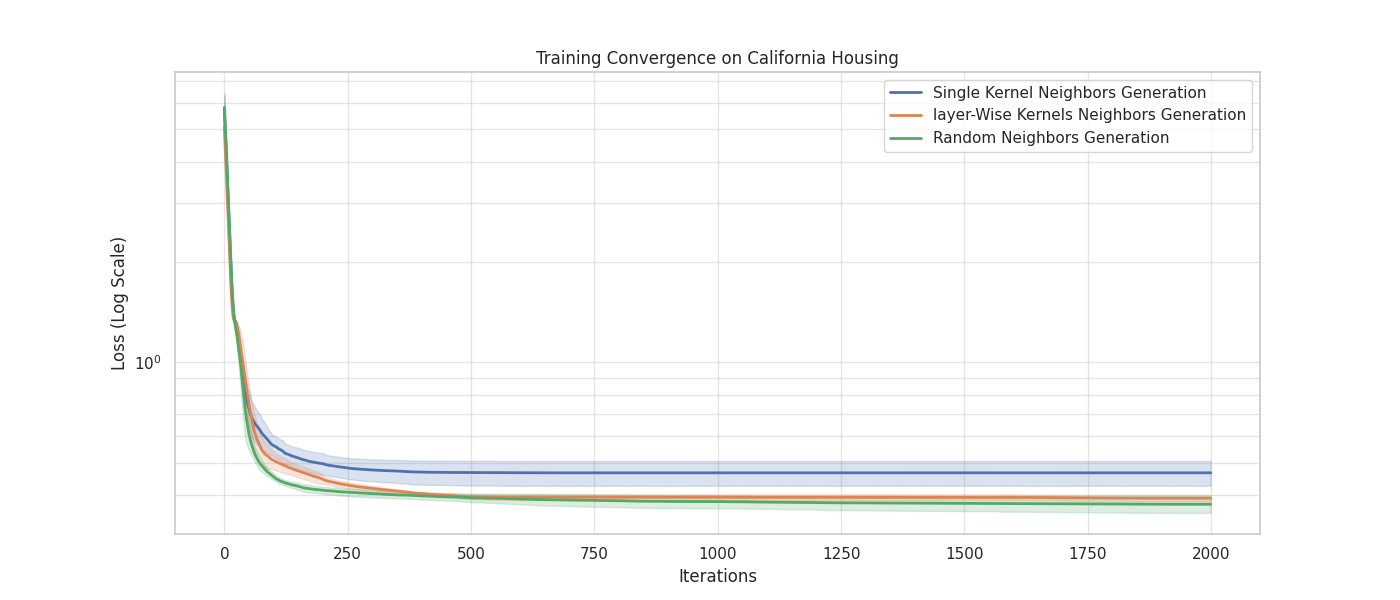
\includegraphics[width=0.9\textwidth]{figures/results/big_net_neighbors_generation_strategies_comparison_with_BS/big_net_neighbors_generation_strategies_comparison_with_BS_convergence.png}
    \caption{Confronto della convergenza per Big Net con Beam Search (Scala Logaritmica).}
    \label{fig:big_net_comp_bs_convergence}
\end{figure}

Nonostante l'estrema complessità del search space, la strategia \textit{Random Neighbors Generation} (linea verde) si conferma la più efficace, raggiungendo la loss finale più bassa. È interessante notare come la curva del metodo \textit{Layer-wise} (linea arancione) si posizioni stabilmente al di sotto del \textit{Single Kernel}, suggerendo che per reti di queste dimensioni, la flessibilità di avere kernel specifici per ogni layer permetta una discesa più accurata rispetto a un approccio a kernel singolo.

\newpage

La stabilità delle prestazioni è analizzata nel boxplot della Figura \ref{fig:big_net_comp_bs_final_loss}.

\begin{figure}[htbp]
    \centering
    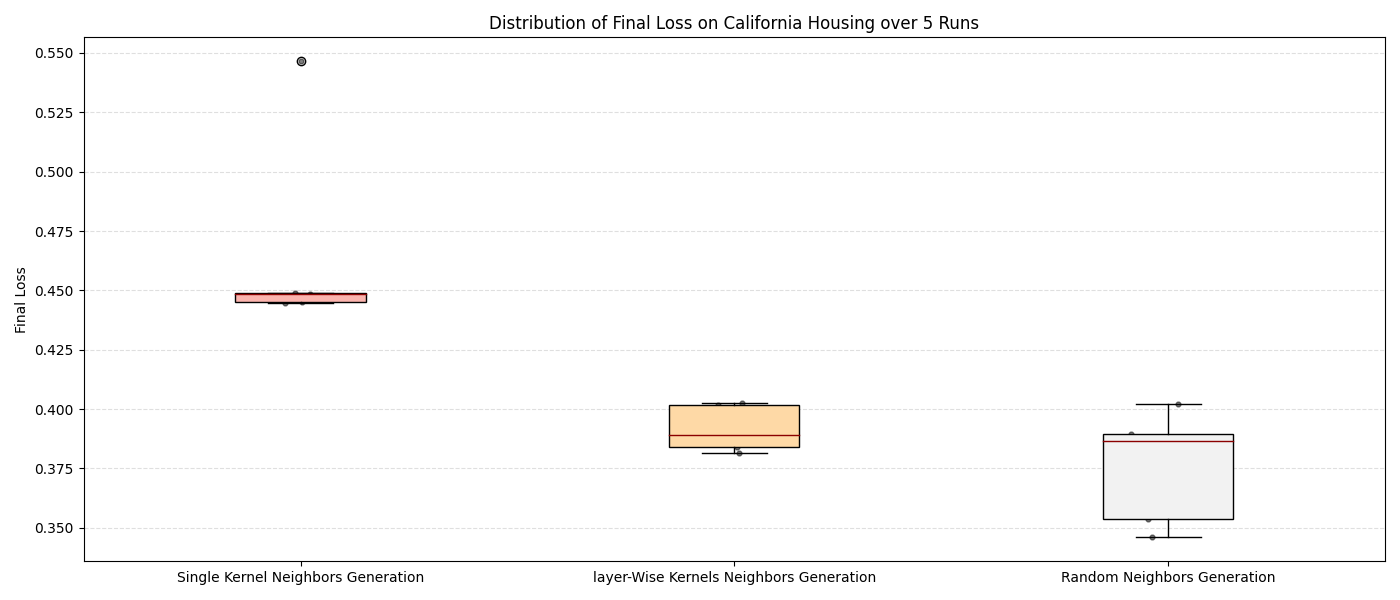
\includegraphics[width=0.85\textwidth]{figures/results/big_net_neighbors_generation_strategies_comparison_with_BS/big_net_neighbors_generation_strategies_comparison_with_BS_final_loss.png}
    \caption{Distribuzione della Loss Finale con Beam Search per Big Net.}
    \label{fig:big_net_comp_bs_final_loss}
\end{figure}

Il metodo Random ottiene la loss media minima ($0.3756$), ma mostra una varianza superiore rispetto al metodo \textit{Layer-wise} ($0.3918$), il quale si dimostra estremamente consistente (Std: $0.0089$). Il metodo \textit{Single Kernel} chiude con la performance meno brillante e la varianza più elevata, confermando le difficoltà dei kernel statici non ottimizzati per layer nel gestire un numero così elevato di parametri.

\newpage

\subsubsection{Metrics Distribution and Predictive Performance}

La Figura \ref{fig:big_net_comp_bs_metrics_dist} illustra la distribuzione delle metriche di regressione per la Big Net.

\begin{figure}[htbp]
    \centering
    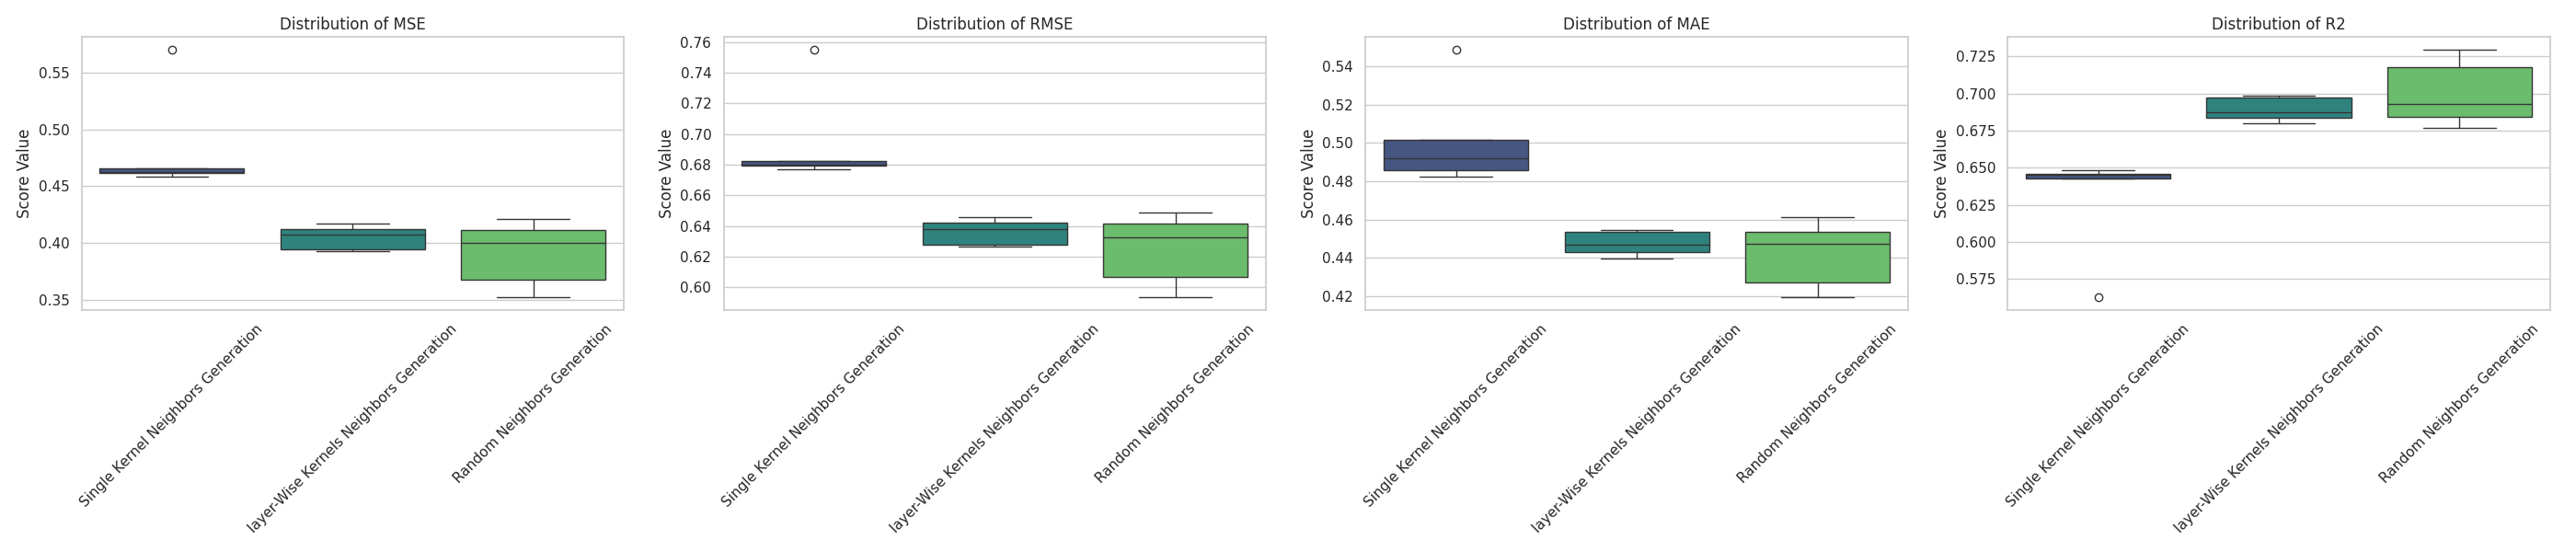
\includegraphics[width=1\textwidth]{figures/results/big_net_neighbors_generation_strategies_comparison_with_BS/big_net_neighbors_generation_strategies_comparison_with_BS_metrics_distribution.png}
    \caption{Distribuzione delle metriche di regressione con Beam Search per Big Net.}
    \label{fig:big_net_comp_bs_metrics_dist}
\end{figure}

I risultati di $R^2$ evidenziano che il metodo Random raggiunge punte medie di $0.7003$, seguito da vicino dal metodo \textit{Layer-wise} con $0.6893$. Il divario tra le strategie si assottiglia rispetto alle reti più piccole, indicando che la potatura operata dalla Beam Search e la corretta configurazione dei kernel per layer rendono i metodi deterministici molto più competitivi su larga scala.

\subsubsection{Summary Statistics}

I dati numerici medi per la Big Net con Beam Search sono riportati nella Tabella \ref{tab:big_net_comp_bs_results}.

\begin{table}[h]
\centering
\scriptsize
\begin{tabular}{|l|c|c|c|}
\hline
\textbf{Metric (Avg)} & \textbf{Random (0.1 / 0.05)} & \textbf{Single Kernel} & \textbf{Layer-wise Kernels} \\ \hline
Avg Final Loss        & 0.3756                       & 0.4668                 & 0.3918                      \\ \hline
Avg Time (s)          & 15623.76                     & 8694.52                & 12999.59                    \\ \hline
Avg MSE               & 0.3906                       & 0.4837                 & 0.4049                      \\ \hline
Avg RMSE              & 0.6247                       & 0.6949                 & 0.6363                      \\ \hline
Avg MAE               & 0.4418                       & 0.5023                 & 0.4475                      \\ \hline
Avg $R^2$             & 0.7003                       & 0.6289                 & 0.6893                      \\ \hline
\end{tabular}
\caption{Confronto statistico medio delle strategie con Beam Search per Big Net.}
\label{tab:big_net_comp_bs_results}
\end{table}